% ---- ETD Document Class and Useful Packages ---- %
\documentclass{ucetd}
\usepackage{subfigure,epsfig,amsfonts}
\usepackage{natbib}
\usepackage{amsmath}
\usepackage{amssymb}
\usepackage{amsthm}
% Add extra packages I need
% Packages used by pandoc when converting Markdown to LaTeX
\usepackage{fixltx2e}
\usepackage{longtable}
\usepackage{booktabs}
% Make cross-references hyperlinks (also format URLs with \url).
% Specify breaklinks so that titles in table of contents linewrap.
\usepackage[breaklinks]{hyperref}
% Fix to use hyperref with UCETD template (from Jason Torres)
\renewcommand{\etdChapterHeadFormat}[1]{\uppercase{#1}}
% Ability to split long captions across pages
\usepackage{ccaption}
% Crop figures
\usepackage{graphicx}
% Add footnote to List of Tables about the supplementary files
\renewcommand{\listtablename}{List of Tables
  \footnote{Note: Due to the large size of most of the tables, the tables
  have been provided in a supplementary file accompanying the
  dissertation.
}}
% Nice tilde
% http://tex.stackexchange.com/questions/9363/how-does-one-insert-a-backslash-or-a-tilde-into-latex/9372#comment47661_9372
\newcommand{\mytilde}{\raise.17ex\hbox{$\scriptstyle\mathtt{‌​\sim}$}}


%% Use these commands to set biographic information for the title page:
\title{Interrogating the 3D structure of primate genomes}
\author{Ittai Ethan Eres}
\department{Human Genetics}
\division{Biological Sciences}
\degree{Doctor of Philosophy}
\date{December 2020}

%% Use these commands to set a dedication and epigraph text
\dedication{Dedication Text}
\epigraph{"'If I am not for myself, who will be for me? \\
But if I am only for myself, who am I?\\
And if not now, when?\\
\
\emph{Rabbi Hillel}}


\begin{document}
%% Basic setup commands
% If you don't want a title page comment out the next line and uncomment the line after it:
\maketitle
%\omittitle

% These lines can be commented out to disable the copyright/dedication/epigraph pages
\makecopyright
%\makededication
%\makeepigraph


%% Make the various tables of contents
\tableofcontents
\listoffigures
\listoftables

% Enter Acknowledgements here
\acknowledgments

I would like to express extreme gratitude to all the people who supported, guided, mentored, and assisted me before and throughout my PhD. None of this work would have been possible without the mental, emotional, and fiscal support of numerous other trainees and faculty.

I am very thankful to my advisor, Yoav Gilad. Our interactions and conversations throughout the course of the PhD have not only significantly shaped my scientific thinking, but have also made my grad school experience an enjoyable and educational one. I found Yoav as an advisor to be a very understanding and compassionate, two qualities that made for a very enriching training experience. I am especially grateful that he encouraged me to pursue comparative primate genomics through the lens of my own interest in 3D genomics, while also always keeping me grounded in pursuing tangible results and publication. Additionally, Yoav was flexible and versatile when it was most needed (i.e. during the COVID-19 pandemic), and helped ensure I was still able to do quality scientific work and graduate. In so many ways, I could not have asked for a better PhD advisor.

I am also thankful to my thesis committee members, Marcelo Nobrega, John Novembre, and Xin He. Their guidance and insight throughout our committee meetings helped steer me in the right direction to make interesting inferences from my data, and, ultimately, to graduate. I also greatly enjoyed our "big picture" discussions at these meetings, that helped contextualize my work in the broader space of epigenetics, evolution, and 3D genome structure. Additionally, I am thankful to Matthew Stephens for his statistical advice and explanations at different times throughout my PhD.

I would like to thank my collaborators, Kevin Luo, Lauren Blake, and Joyce Hsiao. Kevin was instrumental in helping direct my early analyses of Hi-C data, especially with respect to quality control metrics. Lauren and Joyce were both extraordinarily helpful for properly carrying out the mediation analysis assessing the effect of 3D chromatin structure on gene expression differences.

In general, I would like to thank all members of the Gilad lab. My time in the lab was an extremely enjoyable and educational experience. I would like to give special thanks to Bryan Pavlovic for mentoring me early on in my PhD studies. Numerous other lab members provided helpful scientific guidance and were great friends to me during my time in the lab; in particular I would like to thank Jonathan Burnett, Nick Banovich, Seb Pott, Genevieve Housman, Kenneth Barr, Benjamin Fair, Ben Umans, Reem Elorbany, Katie Rhodes, Wenhe Lin, Erik McIntire, Sidney Wang, Courtney Burrows, Po-Yuan Tung, John Blischak, Briana Mittleman, Natalia Gonzales, Irene Gallego Romero, Amy Mitrano, Emilie Briscoe, Stephanie Lozano, Marsha Myrthil, and Claudia Chavarria. I am also grateful to other members of the broader human genetics community during my time at University of Chicago:  Abhishek Sarkar, Joe Marcus, Arjun Biddanda, Nick Knoblauch, Kevin Magnaye, Sarah Urbut, Oni Basu, Vincent Lynch, and countless other trainees, faculty, and staff.

A wide variety of different administrators provided me with unparalleled support during my PhD. I am especially thankful to Sue Levison, who has always gone above and beyond the call of duty to make me and other students feel welcome, and often helped assuage my worries. I would also like to thank Diane Hall, Melissa Lindberg, Candice Lewis, Anita Williams, and Carolyn Brown. In the first few years of my PhD, I was lucky to be funded by the Genetics and Regulation Training Grant (T32GM007197) from the National Institutes of Health. Many thanks to the NIH and to Lucia Rothman-Denes, the grant manager.

I would like to thank my various friends throughout grad school who provided many different kinds of support: Andrew Tremain, Amelia Joslin, UnJin Lee, Frances Lee, Charlie Lang, Erin Fry, Katie Mika, Aarti Venkat, Ryan Duncombe, Chris Stamper, Jess Fessler, Andr�s Moya-Rodriguez, Keelan Armstrong, Ben Ward, Addison Hughes, Michael Hustedde, Drew Waford, Asher Mayerson, Max Sloan, Sam Broer, Seth Brown, Paul Finkelstein, Alex Advani, Toufic Mayassi, Sangman Kim, Jason Lui, Logan Poole, Charlie Dulberger, and countless others. I am also grateful for the different groups that I played both IM and pick-up soccer with throughout grad school. Finally, I would like to thank my partner, Hannah Morley, for the many different ways in which she has supported me throughout this process.

Lastly and most importantly, I would like to thank my family. My parents, Avichai and Ronit, supported me in so many different ways growing up, and gave me the educational and experiential opportunities that enabled me to pursue a PhD to begin with. I could not be more grateful for all their support throughout my life. My siblings, Tomer and Merav, have also been instrumental to my development both emotionally and intellectually, and I am thankful for the different ways in which they have supported and lifted me up. None of what I have accomplished would have been possible without the amazing support my whole family has continuously provided, and I am forever indebted to them.

% Enter Abstract here
\abstract
A primary goal in human genetics is to understand how genetic variation affects phenotypic variation observed between different individuals.  Elucidating these connections is crucial to understanding the molecular mechanisms and causes that lead to differences in traits and diseases among humans, and enables the discovery of therapeutic interventions that can improve human health. Many of the genetic variants associated with trait variation thus far are in non-coding regions of the genome, emphasizing a need to characterize non-coding sequence elements through functional genomics approaches. As opposed to variation in protein-coding sequences, genetic variation at non-coding loci has not been decoded, impeding a rapid understanding of its downstream functional effects. What is clear is that many non-coding loci are likely implicated in gene regulation, and understanding precisely what they are and how they act will require application of a wide variety of functional genomics techniques. In particular, one emerging technique assesses 3D genome structure, which can help connect regulatory loci to the genes they affect, and is rapidly expanding our understanding of gene regulatory networks and the noncoding genome. Various epigenetic features, such as 3D genome structure, can now be compared genome-wide across humans and non-human primates, broadening our understanding of evolution and gene regulation. My thesis work uses these paradigms to understand the interplay between 3D chromatin organization and gene expression across evolution. In Chapter 2, I apply RNA sequencing and chromosome conformation capture sequencing to human and chimpanzee induced pluripotent stem cells, in order to understand how divergence in 3D regulatory landscapes across these species affects expression divergence. As expected, this work demonstrates that reorganization of 3D genome structure contributes to gene regulatory evolution in primates. In Chapter 3, I critically assess existing evidence from other studies that have led many to conclude there is high evolutionary conservation of topologically associating domains (TADs, a large-scale feature of 3D genome organization). A thorough examination of the available data suggests such a conclusion may be unwarranted. Finally, in Chapter 4, I summarize the insights gained from this work, assess the state of the 3D genome field in general, and suggest next steps for future research.

\mainmatter
% Main body of text follows

% Chapter 01 - Introduction
\chapter{Introduction}

\section{The evolution of gene regulation}

The study of human genetics seeks to understand the genetic basis behind human phenotypic variation. Specifically, human geneticists are interested in characterizing how genetics impacts differences in traits between species, as well as between individuals within our own species. Insights gleaned from this field of study are useful not only for understanding and potentially improving human health, but also for furthering our understanding of biology and evolution more broadly. One particularly compelling approach that addresses both these aims is to compare genetic and phenotypic variation between humans and closely-related primate species. Early comparisons between the human and chimpanzee genomes revealed that the two species share the vast majority (99\%) of their DNA, with an especially high level of conservation in protein-coding sequences \cite{King&Wilson + "great ape genetic diversity and population history" + "Initial sequence of the chimpanzee genome and comparison with the human genome"}. These observations provided amazing evolutionary insight, suggesting that differences observed between humans and chimpanzees are not driven by inherent differences in the proteins (genes), but, rather, by differences in how, when, and where these proteins are expressed--i.e. differences in gene regulation \cite{King&Wilson}. More recently, genome-wide association studies (GWAS) within the human species have connected inter-individual differences in traits and diseases with thousands of genetic variants, the vast majority of which are non-coding \cite{Edwards et al 2013 (Beyond GWASs: Illuminating the Dark Road from Association to Function), Gloss and Dinger 2018 (Realizing the significance of noncoding functionality in clinical genomics)}. Additionally, numerous estimates suggest the human genome is comprised of up to 98\% noncoding DNA, much of which is functional, \cite{Pennacchio et al. 2013 (Enhancers: 5 essential ?s), Comfort 2015 (Genetics: We are the 98%), Kellis et al. 2014 (Defining functional DNA elements in the human genome), Consortium 2001 (Initial sequencing and analysis of the human genome), Little 2005 (Structure and function of the human genome)}, further underscoring the importance of understanding gene regulation.

The hypothesis that gene regulatory differences may be major drivers of phenotypic variation was first posited more than 50 years ago \cite{Britten and Davidson 1969+1971}. Although there is still some debate about the extent to which adaptation and speciation are driven by mutations in gene regulatory loci vs. mutations in protein-coding genes \cite{Hoekstra and Coyne 2007, Sean B Carroll 2008}, it is evident that gene expression variance plays a crucial role in phenotypic divergence within and between species \cite{Sean B Carroll 2005, Greg Wray 2007 (evolutionary significance of cis-regulatory mutations), Gilad et al. 2006 (expression profiling in primates...), Frankel Wang and Stern 2012 (Conserved regulatory architecture...), Stern and Orgogozo 2008 (The loci of evolution...), Zheng et al. 2011 (Regulatory variation within and between species)}. Advances in molecular biology and sequencing technologies over the last several decades have enabled rigorous investigations of gene expression levels and the regulatory mechanisms affecting them. RNA-sequencing (RNA-seq) represents a major improvement over prior microarray technology for accurate genome-wide measurement of gene expression levels and other transcriptomic phenotypes  \cite{Zhao et al 2014 (Comparison of RNA-seq and Microarray...activated T cells), Mantione et al 2014 (Comparing Bioinformatic gene expression...), Wang et al. 2009 (RNA-seq: a revolutionary tool for transcriptomics), Marioni et al 2008 (RNA-seq: an assessment of technical reproducibility and comparison with gene expression arrays)}. Simultaneously, an array of emerging molecular and computational techniques allow for genome-wide assessment of different regulatory mechanisms such as DNA methylation, histone modification, chromatin state, transcription factor binding, and more \cite{Chen et al. 2017 (Epigenetic Regulation: A new frontier for biomedical engineers)}. Widespread use of these techniques is needed, because, in contrast to protein-coding genes, there is no clear code connecting primary sequence to downstream function for the noncoding portions of the genome. The outstanding challenges are thus to characterize the different genetic and epigenetic mechanisms regulating gene expression, to understand their relative evolutionary contributions to adaptation and speciation, and to ultimately connect them back to variation in primary DNA sequence.

While my work and this introduction focuses on inter-species primate comparative genomics in order to understand the evolution of gene regulation, it should be noted that research on gene expression differences within species has yielded valuable insights, suggesting expression levels are heritable and connected to genetic variation through expression quantitative trait loci (eQTLs) \cite{Majewski and Pastinen 2010 (The study of eQTL variations...), Gilad, Rifkin, and Pritchard 2008 (Revealing the architecture...)}. These findings further highlight the functional relevance of gene expression levels as a molecular phenotype affecting higher-order traits, providing a tractable avenue for understanding the evolution of a wide variety of phenotypes. In the rest of this introduction, I will review key findings from comparative primate genomics studies about the evolution of gene regulation, and explain why characterizing the 3-dimensional structure of the genome is a critical next step in understanding the evolution of gene regulation and the relationships between genotypes and phenotypes.

\section{Gene regulatory evolution insights from comparative primate genomics}

\textit{Why focus on primates?} Numerous efforts have made progress in decoding the non-coding genome and furthering our understanding of gene regulation. In particular, work from the ENCODE (Encyclopedia of DNA Elements) consortia and many others have helped to identify and characterize functional regulatory elements across a number of species, including humans \cite{Bernstein et al 2010 (The NIH Roadmap Epigenomics Mapping Consortium), ENCODE Project Consortium 2012 (An integrated...in the human genome), Mouse ENCODE Consortium 2012 (An encyclopedia of mouse DNA elements), Celniker et al. 2009 (Unlocking the secrets of the genome)}. Inter-species comparative genomics studies have been especially effective in identifying functional regulatory sequences \cite{Nobrega and Pennacchio 2004 (Comparative genomic analysis as a tool for biological discovery)}. In addition to characterizing specific regulatory loci, studies in model organisms have also revealed that expression divergence between species is primarily driven by mutations in cis-regulatory elements (CREs), rather than trans elements \cite{Tirosh and Barkai 2011 (Inferring regulatory mechanisms...)}. The former operate in an allele-specific manner, typically on the same chromosome, while the latter operate more broadly and can often diffuse throughout the genome. Although these research endeavors have expanded knowledge on gene regulatory mechanisms and associated loci more broadly, their use of distantly-related species precludes the possibility of categorizing their findings as highly conserved or human-specific \cite{Prime time for Primate Functional Genomics}. Grounding genetic and epigenetic observations in humans by comparison with closely-related non-human primates (NHP) is crucial for providing evolutionary context. Without such comparisons, it is impossible to obtain a comprehensive understanding of how different loci and mechanisms of gene regulation have evolved in the human lineage, and, consequently, how these features may affect human-specific phenotypes \cite{Romero, Ruvinsky, and Gilad 2012}. In addition to providing evolutionary context, using NHP in comparative genomics and biomedical research can yield useful insights into human diseases, which are harder to model in more distantly related species with more divergent physiologies \cite{Rogers and Gibbs 2014 (Comparative primate genomics: emerging patterns of genome content and dynamics)}. There are thus a number of different ways in which comparative genomics studies utilizing NHP may provide unique insights into human evolution and the lexicon of human gene regulation, that cannot be obtained by focusing exclusively on model organisms and/or more distantly related species.

However, using primate comparative genomics to understand gene regulation still entails a number of challenges. The paucity of human and chimpanzee primary tissues, as well as obvious ethical limitations on experimentation in the two species, represent major barriers in the study of gene regulation \cite{Romero, Ruvinsky, and Gilad 2012}. Comparison of biological samples between primate species is possible with post-mortem collection of flash-frozen tissues, but this approach is problematic for several reasons. Due to the inherently opportunistic sample collection, sample sizes are typically quite small, with some studies using only a few individuals from each species \cite{Blekhman et al 2008 (Gene regulation in primates evolves under...), Pai et al 2011 (A genome-wide study of DNA methylation), Prescott et al 2015 (Enhancer Divergence...Chimp Neural Crest)}. Additionally, post-mortem tissue samples may be subject to variance induced by technical factors such as sample collection and shipping \cite{Blake et al. 2020 (A comparison of gene expression and DNA methylation), Chevyreva et al. 2007 (Assessing RNA quality in postmortem human brain tissue)}. These issues may be mitigated by utilizing induced pluripotent stem cells (iPSCs), which can be reprogrammed from and differentiated into a wide variety of different cell types \cite{Takahashi & Yamanaka 2006, Takahashi et al. 2007 (Induction of pluripotent stem cells...), Sun et al 2009 (Feeder-free derivation...))}, allowing for controlled experimentation on larger panels of human and NHP cells \cite{Romero et al 2015 (A panel of induced pluripotent stem cells from chimpanzees...), Marchetto et al. 2013 (Differential L1 regulation...)}. Regardless of the biological samples being compared, care must also be taken in the study design and analysis methods employed in a comparative genomics setting. Without careful study design, batch effects may have a strong impact on the data, leading to inferences and conclusions that are driven more by technical variables than by true biological differences. In one intriguing recent example, researchers observed gene expression data from human and mouse clustering by species, rather than by tissue (as would be expected based on prior research) \cite{Mouse ENCODE Consoritum, An Encyclopedia of DNA Elements in the Mouse Genome}. A reanalysis of the data found that this unexpected observation was due to flawed study design confounding sequencing batch with species, and that the data do indeed cluster by tissue after accounting for sequencing batch effects \cite{Gilad and Mizrahi-Man 2015}. With respect to the analysis of comparative genomics data, thoughtful normalization and orthology-calling techniques must also be employed to ensure comparisons made between sequences and features lead to valid biological inferences \cite{Vallender 2009 (Bioinformatics approaches to identifying orthologs and assessing evolutionary relationships), Zhou et al. 2019 (A statistical normalization method and differential expression analysis for RNA-seq data between different species), Blekhman et al. 2010 (Sex-specific and lineage-specific alternative splicing in primates), Cain et al. 2011 (Gene expression differences among primates are associated with changes in a histone epigenetic modification)}. Intentional study designs, sample collection methods, and analytical techniques can attenuate many of the aforementioned limitations.

Even when researchers do well to address technical limitations and minimize confounding variables, there are still challenges in inferring regulatory evolutionary dynamics from comparative primate genomics studies. Numerous models and methodologies exist to infer the action of natural selection on primary DNA sequence \cite{Vitti Grossman and Sabeti 2013, Detecting Natural Selection in Genomic Data}. Such methods are particularly effective when applied to protein-coding genes, where the functional effect of a mutation can be understood readily, given our knowledge of the link between sequence codons and the amino acids they are translated into. However, the links between primary sequence and trait variation are considerably less clear in the context of epigenetic, regulatory, and other molecular phenotypes. In these cases, the action of natural selection on the trait in question can be inferred and statistically tested based on observed deviations from null models (e.g. a neutral model with no selection). These types of approaches can be extremely useful in model organisms, where one can directly measure the necessary parameters (e.g. mutation rate) to generate a reasonable null model \cite{Gilad Oshlack and Rifkin 2006, Natural selection on gene expression}. Unfortunately, these parameters are difficult to measure even in model organisms, and can often be practically impossible to estimate in humans and NHP. For most functional genomic traits that are studied, there is not yet a robust, well-formulated null model of no selection. Thus, more ad-hoc and empirical approaches must be utilized to understand the action of natural selection on intermediate molecular phenotypes. For instance, if gene expression levels show low variation both within and between species, it may be inferred that regulation of these genes is evolving under stabilizing selection (i.e. expression extremes are selected against). Conversely, if expression variance is low within species, but mean expression is much higher or lower in one species compared to others, this may suggest directional selection is affecting regulation of the gene in that species \cite{Romero, Ruvinsky, and Gilad 2012}. Empirical approaches such as these can therefore elucidate evolutionary dynamics, but greater care must be taken in interpretation of their results. In the previous example, more extreme expression in one species may actually be due to environmental factors and/or reduced action of stabilizing selection on that lineage, rather than directional selection. Functional follow-up studies, consideration of interspecies environmental differences, and accounting for different possible evolutionary trajectories can help exclude alternative explanations for specific evolutionary inferences. Consequently, when executed and interpreted properly, comparative primate genomics studies have vastly expanded our understanding of the mechanisms and loci involved in the evolution of gene regulation.

\textit{What have we learned?}
For many genes, results from comparative studies suggest that expression levels in primates are evolving under natural selection \cite{Khaitovich et al 2006 (Evolution of primate gene expression), Blekhman et al 2008 (Gene regulation in primates evolves under tissue-specific selection pressures), Brawand et al 2011 (The evolution of gene expression levels in mammalian organs)}. One early study looked at RNA levels in liver tissues from humans, chimpanzees, orangutans, and rhesus macaques, finding a set of genes with relatively invariant expression levels across species \cite{Gilad et al 2006 (Expression profiling in primates...)}. If regulatory mutations are in general selectively neutral (as many other mutations have been speculated to be \cite{Kimura 1968 (Evolutionary rate at the molecular level)}), expression levels for most genes would show more substantial inter-primate variation. The observed low variance in expression across diverse primate lineages suggests stabilizing selection has acted on these genes, preventing extreme expression levels \cite{Lemos et al 2007, Rates of divergence in gene expression profiles of...}. Other studies comparing RNA levels across primate species have largely corroborated this notion \cite{Blekhman et al 2008, Perry et al. 2011 (Comparative RNA sequencing reveals...), Brawand et al 2011, Chen et al. 2018 (A quantitative framework for characterizing the evolutionary history of mammalian gene expression)}. It is interesting to note that interspecies conservation of expression levels is particularly high for genes thought to be critical for defining cell type identity. In turn, gene expression patterns are more similar in the same tissue across different species than across different tissues within a species \cite{Sudmant et al. 2015 (Meta-analysis of RNA-seq expression data...)}. Taken together, these results bolster the idea that regulatory changes may be crucial drivers of evolution and adaptation. Compared to protein-coding sequence mutations, regulatory mutations can act in a more tissue-specific manner, and are thus less susceptible to pleiotropic effects that could be deleterious across multiple organs \cite{Wilson et al. 1974 (Two types of molecular evolution...), Blekhman et al 2008}.

While most genes show evidence for their expression evolving under stabilizing selection in primates, there has also been great interest in finding examples of directional selection. The impact of such examples is fairly intuitive: a strong motivation in comparative primate genomics is to identify the genetic and epigenetic facets underlying differences between humans and NHP, in an effort to understand the biology behind human-specific traits and diseases. The exact proportion of genes whose regulation appears to be evolving under directional selection in primates differs dependent upon the tissue or cell type being considered, but still represents the minority of genes \cite{Romero, Ruvinsky and Gilad 2012}. As discussed above, not every gene showing lineage-specific expression differences compared to other primates is necessarily evolving under positive (directional) selection on its regulation, but many likely are. Since some of the most striking phenotypic differences between humans and NHP are cognitive, many primate comparative genomics studies have focused on the brain and specific cell types therein \cite{Nowick et al 2009 (Difference in human and chimpanzee gene expression patterns define an evolving network of transcription factors in brain), Giger et al. 2010 (Evolution of Neuronal and Endothelial Transcriptomes in Primates)}. Results from studies utilizing bulk RNA-seq \cite{Somel et al 2009 (Transcriptional neoteny in the human brain)}, and from more recent work examining RNA transcripts in single cells \cite{Mora-Bermudez et al. 2016 (Differences and similarities between human and chimpanzee neural progenitors...), Zhu et al. 2018 (Spatiotemporal transcriptomic divergence across human and macaque brain development), Sousa et al. 2017 (Molecular and cellular reorganization of neural circuits in the human lineage)}, suggest that interspecies expression variation in tissue location (heterotopy) and timing (heterochrony) during brain development may play a role in cognitive differences observed between humans and NHP. There are also examples in other organs of directional selection acting on gene regulation. An RNA-seq study on livers from 16 species revealed expression changes in some primate lineages that could be tied to dietary adaptations \cite{Perry et al 2011 (Comparative RNA sequencing reveals substantial...)}. A similar study examining livers, kidneys, and hearts in humans, chimpanzees, and rhesus macaques found subsets of genes in each tissue displaying lineage-specific expression in humans \cite{Blekhman et al 2008}. Yet another study found marked expression differences in blood leukocytes, livers, and brains of humans, chimpanzees, orangutans, and rhesus macaques \cite{Enard et al 2002 (Intra- and Interspecific Variation in Primate Gene Expression Patterns)}. A more recent study assayed RNA levels in heart, kidney, liver, and lung tissue samples from humans, chimpanzees, and rhesus macaques, and also found a minority of genes whose expression patterns imply some directional selection \cite{Blake et al. 2020 (A comparison of gene expression and DNA methylation patterns...)}. Specific and functionally validated examples of genes with expression levels evolving under directional selection are scarce, and it is difficult to confidently connect them to higher-order phenotypes \cite{Babbitt et al 2010 (Multiple functional variants in cis modulate PDYN expression), Warner et al. 2009 (Functional consequences of genetic variation in primates on tyrosine hydroxylase (TH) expression in vivo)}. More examples will hopefully be discovered and characterized as our understanding of gene-phenotype connections increases, and as single-cell and other technologies enable better sampling from different locations, time points, and, consequently, cell types within a tissue. Regardless, numerous lines of evidence from inferences about directional selection suggest that a complex network of different mechanisms regulates gene expression. Gene sets with some evidence for directional selection on their regulation are often enriched for transcription factors \cite{Blekhman et al 2008, Gilad et al. 2006 (Expression profiling in primates revels a rapid evolution of human transcription factors)}, are regulated by fewer enhancers than genes with more conserved expression patterns \cite{Danko et al 2018 (Dynamic evolution of regulatory element ensembles in primate CD4+ T cells), Berthelot et al. 2018 (Complexity and conservation of regulatory landscapes underlie evolutionary resilience of...)}, and do not necessarily display signatures of directional selection in the abundance of their corresponding proteins \cite{Khan et al 2013 (Primate transcript and protein expression levels evolve under compensatory selection pressures)}. This last observation is particularly intriguing, and suggests that protein levels may be under more selective constraint than RNA levels and other gene regulatory mechanisms \cite{Wang et al 2018 (Post-translational buffering leads to convergent protein expression levels between primates), Anderson Vigalys and Tung 2020 (Broadening primate genomics: new insights into the ecology and evolution of primate gene regulation)}. An emerging notion from this and other work is that regulatory mechanisms utilize such buffering and redundancy to ensure appropriate downstream functional outcomes \cite{MacNeil and Walhout 2011 (Gene regulatory networks and the role of robustness and stochasticity in the control of gene expression)}. Together, these findings highlight the importance of measuring a wide variety of epigenetic features in order to understand the evolution of gene regulation.

Indeed, more recent work has moved from merely characterizing expression differences across primate species, to attempting to understand variation in regulatory mechanisms driving these differences. Understanding the regulatory mechanisms and loci responsible for expression variation should help de-mystify the noncoding portions of the genome, identifying functional elements that may have an impact on human health \cite{Cooper and Shendure 2011 (Needles in stacks of needles: finding disease-causal variants in a wealth of genomic data)}. One recent study examined DNA methylation and gene expression in livers, kidneys, hearts, and lungs from humans, chimpanzees, and rhesus macaques, finding that methylation differences can only explain a small proportion of expression variation between tissues and species \cite{Blake et al 2020 (A comparison of gene expression and DNA methylation...)}. An earlier study found similar results when comparing human and chimpanzee livers, hearts, and kidneys \cite{Pai et al 2011 (A Genome-Wide study of DNA methylation...)}. Differential abundance of microRNAs, which regulate mRNA transcript decay, was also observed to account for only a small proportion (<5\%) of expression differences in prefrontal cotex across humans, chimpanzees, and rhesus macaques \cite{Hu et al. 2011 (MicroRNA expression and regulation in human...), Somel et al. 2011 (MicroRNA-driven developmental remodeling in the brain...)}. Alternative splicing of genes, which could (in theory) easily introduce regulatory novelty, has also been shown to have little effect on differential expression between humans and chimpanzees \cite{Calarco et al. 2007 (Global analysis of alternative splicing differences between humans and chimpanzees)}. Comparable observations have been made for histone marks: one early study examined H3K4me3 in lymphoblastoid cell lines (LCLs) from humans, chimpanzees, and rhesus macaques, and found that interspecies differences in this histone modification explain only 7\% of interspecies expression variation \cite{Cain et al 2011 (Gene expression differences among primates are associated with changes in a histone epigenetic modification)}. These results are perhaps not surprising, given that only a small minority of loci show human-specific increase or decrease of H3K4me3 in prefrontal cortex samples from the same species \cite{Shulha et al 2012 (Human-specific histone methylation signatures at transcription start sites in prefrontal neurons)}. A later analysis in LCLs from the same species integrated RNA polymerase II occupancy, H3K4me1, H3k4me3, H3K27ac, and H3K27me3, and found that roughly 40\% of interspecies gene expression variance can be explained by these marks combined \cite{Zhou et al. 2014 (Epigenetic modifications are associated with inter-species gene expression variation in primates)}. Similarly, an even more recent study integrated a wide variety of histone marks as well as chromatin accessibility and methylation status in LCLs from great apes and macaques, and found that these features combined can explain approximately 67\% of interspecies expression variance \cite{Garcia-Perez et al 2020 (Biorxiv, Epigenomic profiling of primate LCLs reveals the coordinated evolution of gene expression and epigenetic signals in regulatory architectures)}. It would thus appear that the effect of any single epigenetic mechanism on gene expression is relatively modest, but, in concert, these mechanisms have a large effect on expression levels.

One principle that emerges from these findings and others in model organisms is that chromatin state and its effects on cis-regulatory elements (CREs) play a major role in the evolution of gene expression \cite{Romero, Ruvinsky and Gilad 2012, Degner et al 2012 (DNase I sensitivity QTLs are...)}. Many of the aforementioned epigenetic modifications and mechanisms are associated with how 'open' or 'closed' chromatin is at a given locus, making the locus and the CREs it encompasses more or less accessible to transcription factors and other regulatory machinery \cite{Calo and Wysocka 2013 (Modification of enhancer chromatin: what, how and why?)}. It is therefore important to assess not only whether a given CRE is conserved, but also if the chromatin state at that locus is comparable across species. A variety of methods exist to assay chromatin accessibility, such as DNase-seq and ATAC-seq \cite{Klein and Hainer 2019 (Genomic methods in profiling DNA accessibility and factor localization), Tsompana and Buck 2014 (Chromatin accessibility: a window into the genome), Buenrostro et al 2015 (ATAC-seq: A method for assaying chromatin accessibility genome-wide)}. Broadly, these methods have found that the vast majority of the genome is not accessible in any given cell type, and that most transcription factor binding events occur within regions of open chromatin identified by these assays \cite{Thurman et al. 2012 (The accessible chromatin landscape of the human genome)}. Consequently, regions of open chromatin are often likely to harbor active regulatory elements \cite{Song et al. 2011 (Open chromatin defined by DNaseI and FAIRE identified regulatory elements that shape cell-type identity), Klemm et al. 2019 (Chromatin accessibility and the regulatory epigenome)}. Consortia such as ENCODE have used ChIP-seq and other techniques to produce copious histone mark and other epigenetic data that, through careful analysis, have helped identify and characterize different classes of CREs at these putative regulatory regions\cite{ENCODE Project Consortium 2012 (An integrated...in the human genome), Li et al. 2018 (Genome-wide prediction of cis-regulatory regions using supervised deep learning methods), Ernst and Kellis 2012 (ChromHMM: automating chromatin-state discovery and characterization), Hoffman et al. 2012 (Unsupervised pattern discovery in human chromatin structure through genomic segmentation)}. Some of the most well-studied CREs are enhancers, DNA modules that interface with transcription factors and associated proteins to make contact with gene promoters, thereby affecting gene expression. Although the measured extent of inter-primate divergence or conservation in enhancers and other CREs is dependent on the technology used and the number of species examined \cite{Edsall et al. 2019 (Evaluating chromatin accessibility differences across multiple primate species using a joint modeling approach), Swain-Lenz et al 2019 (Comparative analyses of chromatin landscape in white adipose tissue suggest humans may have less beigeing...)}, there are intriguing enhancer differences across primate species. Enhancers are considerably less conserved amongst primate lineages than gene expression levels \cite{Villar et al. 2015 (Enhancer evolution across 20 mammalian species), Berthelot et al. 2017 (Complexity and conservation of regulatory landscapes underlie evolutionary resilience of mammalian gene expression)} and less conserved than promoters \cite{Trizzino et al 2017 (Transposable elements are the primary source of novelty in primate gene regulation)}, highlighting their evolutionary relevance. Surveys of enhancers across primate and mammalian evolution have found interspecies differences in their activity \cite{Klein et al. 2018 (Functional characterization of enhancer evolution in the primate lineage), Prescott et al 2015 (Enhancer divergence and cis-regulatory evolution in the human and chimp neural crest), Shibata et al 2012 (Extensive evolutionary changes in regulatory element activity during human origins...)}, and evidence for high evolutionary turnover of enhancers as compared to promoters \cite{Carelli et al 2018 (Repurposing of promoters and enhancers during mammalian evolution), Villar et al. 2015 (Enhancer evolution across 20 mammalian species)}.

While tremendous work has been done to identify and characterize enhancers and other CREs, numerous outstanding questions remain. Identification of enhancers is still imperfect because there is no single epigenetic mark that perfectly predicts enhancer regions. Enhancers affect gene expression via chromatin looping but also through other mechanisms that are less well understood (e.g. enhancer transcription), and disease-associated genetic variation at enhancer regions is difficult to functionally characterize \cite{Enhancers: 5 essential questions}. Although we have been able to map regulatory quantitative trait loci (QTL, genetic variants with discrete effects on expression or other intermediate molecular phenotypes), most disease-associated variants in regulatory regions do not appear as QTL \cite{Umans et al. 2020 (Where are the disease-associated eQTLs?)}. This is likely due in part to sampling strategies (e.g. not assaying gene expression in the appropriate cell type or condition relevant to the disease), but progress in understanding these mutations is also broadly stymied by a lack of knowledge about which gene(s) a given CRE regulates \cite{Umans et al. 2020}. Determining CRE targets is of particular importance both because CREs act in a distance-independent manner (only 40\% of enhancers are linked to the nearest gene \cite{Andersson et al. 2014 (An atlas of active enhancers across human cell types and tissues)}), and because many CREs are tissue-specific in their activity \cite{Levine 2010 (Transcriptional enhancers in animal development and evolution), Ong et al. 2011 (Enhancer function new insights into the regulation of tissue-specific gene expression), Allis et al. 2016 (The molecular hallmarks of epigenetic control), Won et al. 2008 (Prediction of regulatory elements in mammalian genomes using chromatin signatures)}. Ultimately, CREs' tissue-specific effects on gene expression are likely to be principally determined by local chromatin state and by what gene promoter(s) CREs come into contact with \cite{Garcia-Gonzalez et al 2016 (Chromatin remodeling effects on enhancer activity)}. Connecting regulatory elements directly with their targets thus represents a crucial step towards obtaining a complete picture of how CREs modify expression, and how mutations in CREs affect higher-order phenotypes. My thesis work addresses this issue by examining expression divergence between humans and chimpanzees, with a focus on comparative assessment of CRE-gene contacts in 3-dimensional genome space.

\section{The growing importance of the 3D genome}
Given the vast wealth of genomic information that each cell has to carry in its nucleus, eukaryotic genomes must be packaged in a highly complex and structured fashion. At the highest level, individual chromosomes preferentially occupy discrete regions of the nucleus ("chromosome territories"), and these territories are fairly conserved across primate lineages \cite{Meaburn and Misteli 2007 (Chromosome territories), Mora et al. 2006 (Chromosome territory positioning of conserved homologous chromosomes in different primate species), Tanabe et al. 2002 (Evolutionary conservation of chromosome territory arrangements in cell nuclei from higher primates)}. Early studies of 3D genome structure largely relied on imaging techniques such as FISH (fluorescence in-situ hybridization), and did well to uncover chromosome territories; the advent of molecular methodologies like chromosome conformation capture (3C) have enabled interrogation of 3D genome structure at even finer scales \cite{Dekker et al 2002 (Capturing chromosome conformation)}. Since the inception of 3C, the technology has developed through a variety of iterations and improvements that have increased its genomic resolution and throughput \cite{Fraser et al. 2015 (An overview of genome organization and how we got there: from FISH to Hi-C)}. The latest version, known as Hi-C, pairs the original method?s proximity-based ligation with high throughput next-generation sequencing to find DNA-DNA contacts genome-wide \cite{Lieberman-Aiden et al. 2009 (Comprehensive mapping of long-range interactions reveals folding principles of the human genome)}. These techniques have revealed that, beneath the scale of chromosome territories, individual chromosomes are also partitioned into two types of large-scale "compartments": A compartments, representing open and transcriptionally accessible chromatin, and B compartments, representing closed chromatin \cite{Lieberman-Aiden et al. 2009 (Comprehensive mapping of long-range interactions reveals folding principles of the human genome), Naumova and Dekker 2010 (Integrating one-dimensional and three-dimensional maps of genomes)}. At an even finer scale, loci within a compartment appear to form self-interacting regions on the scale of a megabase, termed topologically associating domains (TADs) \cite{Dixon et al. 2012 (Topological domains in mammalian genomes identified by analysis of chromatin interactions), Nora et al. 2012 (Spatial partitioning of the regulatory landscape of the X-inactivation centre), Hou et al. 2012 (Gene density, transcription, and insulators contribute to the partition of the Drosohila genome into physical domains), Sexton et al. 2012 (Three-dimensional folding and functional organization principles of the drosophila genome)}. As I discuss further in the third chapter of this thesis, the definition of a TAD is still changing as Hi-C libraries are more deeply sequenced and new TAD inference algorithms arise. Regardless, loci within a TAD make contact with one another much more frequently than they do with loci outside of the TAD, suggesting that TADs may represented neighborhoods of insulated gene regulation that constrain the possible set of gene-CRE interactions \cite{Andrey and Mundlos 2017 (The three-dimensional genome: regulating gene expression during pluripotency and development), Symmons et al. 2014 (Functional and topological characteristics of mammalian regulatory domains), Sexton and Cavalli 2015 (The role of chromosome domains in shaping the functional genome)}. Lastly and perhaps most importantly, at the lowest scale, Hi-C and related techniques have uncovered individual DNA looping interactions that bring linearly distant CREs into proximity with the genes they regulate \cite{Rao et al. 2014 (A 3D map of the human genome at kilobase resolution...), Kadauke and Blobel 2008 (Chromatin loops in gene regulation)}.

Numerous lines of evidence point to the functional significance of 3D genome organization at different scales. Studies have found that a significant fraction of genomic regions switch between A and B compartments in different ways during organismal development and cellular differentiation \cite{Eijy Nagai et al. 2019 (Analyzing the 3D chromatin organization coordinating with gene expression regulation in B-cell lymphoma), Dixon et al. 2015 (Chromatin architecture reorganization during stem cell differentiation), Zhang et al. 2019 (Transcriptionally active HERV-H retrotransposons demarcate topologically associating domains in human pluripotent stem cells), Luo et al. 2020 (Reorganized 3D genome structures support transcriptional regulation in mouse spermatogenesis)}. Such compartment switching can move individual loci between permissive and repressed states along differentiation pathways, in part explaining regulatory differences between different cell types \cite{Yin et al. 2012 (Global changes in nuclear positioning of genes and intra- and inter-domain genomic interactions that orchestrate B cell fate), Dileep et al. 2019 (Rapid irreversible transcriptional reprogramming in human stem cells accompanied by discordance between replication timing and chromatin compartment)}. Some similar results have been observed in TADs, suggesting TAD locations and intra- and inter-TAD contact frequencies change during cellular development \cite{Chathoth and Zabet 2019 (Chromatin architecture reorganization during neuronal cell differentiation in Drosophila genome), Dixon et al. 2015 (Chromatin architecture reorganization during stem cell differentiation), Fraser et al. 2015 (Hierarchical folding and reorganization of chromosomes are linked to transcriptional changes in cellular differentiation), Bonev et al. 2017 (Multiscale 3D genome rewiring during mouse neural development), Chen et al. 2019 (Spatial genome re-organization between fetal and adult hematopoietic stem cells)}, although the extent of these alterations is less clear given variance in TAD identification \cite{Dali and Blanchette 2017 (A critical assessment of TAD prediction tools)}. Despite uncertainty about the role of TAD variance in cellular differentiation, it is clear that TADs play an important role in genome organization and function. Genes located within the same TAD can have strongly correlated expression patterns and are often co-regulated during cell differentiation \cite{Nora et al. 2012 (Spatial partitioning...), Zhan et al. 2017 (Reciprocal insulation analsis of Hi-C data shows that TADs represent a functionally...), Ramirez et al. 2018 (High-resolution TADs reveal DNA sequences underlying genome organization in flies)}. TAD boundaries are strongly correlated with replication-timing domain boundaries \cite{Pope et al. 2014 (Topologically associating domains are stable units of replication-timing regulation)}, and are enriched for insulator elements such as CCCTC-binding factor (CTCF) \cite{Dixon et al. 2012, Rao et al. 2014}. Disruptions to normative TAD structure have also been implicated in a number of human pathologies \cite{Lupianez et al. 2016 (How alterations of chromatin domains result in disease), Ibn-Salem et al. 2014 (Deletions of chromosomal regulatory boundaries are associated with congenital disease), Franke et al. 2016 (Formation of new chromatin domains determines pathogenicity of genomic duplications)}. Similarly, 3D genome organization at the lowest scale (i.e. individual gene-CRE loops) affects gene expression and regulation \cite{Greenwald et al 2019 (Subtle changes in chromatin loop contact propensity are associated with differential gene regulation and expression), Bartman et al. 2016 (Enhancer regulation of transcriptional bursting parameters revealed by forced chromatin looping), Deng et al. 2014 (Reactivation of developmentally silenced globin genes by forced chromatin looping), Morgan et al. 2017 (Manipulation of nuclear architecture through CRISPR-mediated chromosomal looping)}, and characterizing these interactions helps connect genetic variation with human trait and disease variation \cite{Gamazon et al. (Using an atlas of gene regulation across 44 human tissues to inform complex disease- and trait-associated variation), Montefiori et al. 2018 (A promoter interaction map for cardiovascular disease genetics), Zhao et al. 2020 (Molecular mechanisms of coronary disease revealed using quantitative trait loci for TCF21 binding, chromatin accessibility, and chromosomal looping), Mumbach et al 2017 (Enhancer connectome in primary human cells identifies target genes of disease-associated DNA elements)}. While GWAS have done well to identify variants associated with many human diseases, analysis of chromatin conformation capture data is often necessary to understand understand how these variants exert their effects, which genes and loci they interact with, and, consequently, what therapeutic options may be effective \cite{Fadason et al. 2018 (Chromatin interactions and expression quantitative rait loci reveal genetic drivers of multimorbidities)}. In one particularly compelling example, researchers long thought that an obesity-associated mutation in an intron of the \textit{FTO} gene increased risk of obesity and type 2 diabetes by affecting the gene itself \cite{Grunnet et al. 2009 (Regulation and function of FTO mRNA expression in human skeletal muscle and...)}. This was not an unreasonable assumption, especially since follow-up studies found \textit{FTO} expression levels affect body mass in mice \cite{Church et al. 2010 (Overexpression of FTO leads to increased food intake...), Fischer et al. 2009 (Inactivation of the FTO gene protects from obesity), Gao et al. 2010 (The fat mass and obesity associated gene FTO functions in the brain...)}. Only through the application of chromosome conformation capture was it finally discovered that the variant in question actually regulates the expression of a transcription factor gene several megabases away, \textit{IRX3} \cite{Smemo et al. 2014 (Obesity-associated variants within FTO form long-range functional connections with IRX3)}. There are countless other examples where integration of Hi-C data has aided in identification of novel pathways and genes involved in the progression of various human pathologies \cite{Martin et al. 2015 (Capture Hi-C reveals novel candidate genes and complex long-range interactions with related autoimmune risk loci), Martin et al. 2016 (Identifying Causal Genes at the Multiple Sclerosis Associated Region 6q23 Using Capture Hi-C), Matoba et al. 2020 (Mapping Alzheimer's Disease Variants to Their Target Genes Using Computational Analysis of Chromatin Configuration), Wu and Pan 2018 (Integration of Enhancer-Promoter Interactions with GWAS Summary Results Identifies Novel Schizophrenia-Associated Genes and Pathways)}. Without a doubt, collecting and analyzing chromosome conformation capture data across species and cell types represents an exciting novel frontier in broadening our understanding of gene regulation, development, and evolution.

Overall, there is a dearth of comparative studies examining 3D genome architecture across species. In Chapter 2, I address this gap by collecting, integrating, and analyzing Hi-C and RNA-seq data from human and chimpanzee iPSCs. In Chapter 3, I challenge the prevailing notion that TADs are highly conserved across species by critically analyzing the existing data that support this claim. In the final chapter, I discuss the evolutionary and gene regulatory implications of my findings, before providing some perspective on the state of the 3D genome field and recommendations for future research directions.

% Chapter 02 - First Paper
\chapter{Reorganization of 3D genome structure may contribute to gene regulatory evolution in primates}\label{ch:ch02}

\section[Abstract]{Abstract\footnotemark}

\footnotetext{Citation for chapter: Eres IE, Luo K, Hsiao CJ, Blake LE, Gilad Y. 2019. Reorganization of 3D genome structure may contribute to gene regulatory evolution in primates. PLoS Genetics 15, e1008278. doi:10.1371/journal.pgen.1008278}

A growing body of evidence supports the notion that variation in gene regulation plays a crucial role in both speciation and adaptation. However, a comprehensive functional understanding of the mechanisms underlying regulatory evolution remains elusive. In primates, one of the crucial missing pieces of information towards a better understanding of regulatory evolution is a comparative annotation of interactions between distal regulatory elements and promoters. Chromatin conformation capture technologies have enabled genome-wide quantifications of such distal 3D interactions. However, relatively little comparative research in primates has been done using such technologies. To address this gap, we used Hi-C to characterize 3D chromatin interactions in induced pluripotent stem cells (iPSCs) from humans and chimpanzees. We also used RNA-seq to collect gene expression data from the same lines. We generally observed that lower-order, pairwise 3D genomic interactions are conserved in humans and chimpanzees, but higher order genomic structures, such as topologically associating domains (TADs), are not as conserved. Inter-species differences in 3D genomic interactions are often associated with gene expression differences between the species. To provide additional functional context to our observations, we considered previously published chromatin data from human stem cells. We found that inter-species differences in 3D genomic interactions, which are also associated with gene expression differences between the species, are enriched for both active and repressive marks. Overall, our data demonstrate that, as expected, an understanding of 3D genome reorganization is key to explaining regulatory evolution.

\section{Introduction}\label{ch02-introduction}
A growing body of evidence indicates that variation in gene regulation plays a key role in phenotypic divergence between species \cite{Britten.1971, King.1975, Carroll.2005, Gilad.2006, Wray.2007, Blekhman.2008, Karaman.2003}. Inferring the causal relationship between inter-species regulatory differences and phenotypic differences between species remains challenging, but compelling examples of regulatory adaptations have been published in a large number of species, including primates \cite{Prabhakar.2008, Babbitt.2010, Warner.2009, Loisel.2006, Rockman.2005, Pollard.2006}. The molecular mechanisms that underlie regulatory adaptation have also been the focus of much research. Studies in mice, flies, yeast, and primates have revealed that expression divergence between species is often driven by mutations or epigenetic modifications within cis-regulatory elements (CREs), rather than trans elements (e.g. transcription factors \cite{Wray.2007, Prabhakar.2008, Babbitt.2010, Warner.2009, Loisel.2006, Rockman.2005, Pennacchio.2013, Ong.2011}). This makes intuitive sense, because transcription factors can operate broadly across multiple functional contexts and throughout the genome (affecting many genes), whereas CREs often have more specific functional outcomes \cite{Carroll.2005, Wilson.2009}.

The ability to measure epigenetic marks, chromatin structure, and other functional genomic data has enabled us to identify and classify CREs into different types of regulators with distinct effects on gene expression (e.g. enhancers, silencers, insulators) \cite{Allis.2016, consortium.2012a, Won.2008}. Despite significant advances in our ability to identify and predict the functional role of CREs, we still lack a comprehensive characterization of the functional relationships between CREs and the genes they regulate. In many cases, we still do not know which genes are regulated by which CREs, or when and how often these relationships change. Connecting CREs to their target genes is crucial for understanding how regulatory architecture changes in response to different spatial, temporal and organismal contexts \cite{Ong.2011, Allis.2016, consortium.2012a, Won.2008, Levine.2010, Dowell.2011, Fagerberg.2014}. Ultimately, the effects of CREs on gene expression are likely to depend on which promoter(s) they contact, which is inherently related to the 3D structure of the genome \cite{Fukaya.2016, Huang.2017}.

The proximity and frequency of CRE-gene contacts can be measured in vivo using chromosome conformation capture techniques \cite{Dekker.2002}. Chromosome conformation affects how genes are expressed within a cell \cite{Babaei.2015, Gerstein.2012, Lan.2012, Botta.2010, Dong.2010, Homouz.2013, Jin.2013, Rao.2017}. For example, 3D genome structures may bring linearly distant loci into close proximity, connecting genes with CREs \cite{Shen.2012, Rieder.2012, Cremer.2001, Sexton.2007, Dekker.2008, Misteli.2007, Kosak.2004}. Expressed genes have been observed to spatially localize with distant CREs in 3D FISH experiments \cite{Rieder.2012, Schoenfelder.2010}. The latest chromosome conformation capture based technique, Hi-C, pairs the original method's proximity-based ligation with high-throughput sequencing to identify DNA-DNA contacts on a genome-wide scale \cite{Lieberman-Aiden.2009}. With enough sequencing coverage, Hi-C data can ultimately yield a comprehensive map of the 3D structure of an entire genome at high resolution \cite{Varoquaux.2014}.

Divergence in 3D genome structure may lead to regulatory evolution and ultimately to adaptation of new phenotypes. Currently, however, there are only a small number of comparative Hi-C data sets that can be used to test this notion \cite{Rudan.2015, Rao.2014, Dixon.2012}, and even fewer comparative data sets in primates \cite{Darrow.2016, Lazar.2018}. Most Hi-C studies to date have focused primarily on variation in chromatin contact frequencies within a single species \cite{Lieberman-Aiden.2009, Schmitt.2016, Kim.2017, Li.2015}. The few comparative Hi-C studies published to date typically draw comparisons between distantly related species (such as human and mouse \cite{Rao.2014, Dixon.2012}), use cancerous or otherwise transformed cell lines \cite{Rao.2014}, and rely on low resolution genome-wide Hi-C data (typically collecting 100-600M reads from most samples \cite{Rudan.2015, Dixon.2012, Dong.2017}). These comparative studies typically collect data in only a single individual from each species, and often compare contacts that are inferred from Hi-C libraries with large differences in read depth between species, a property that leads to differences in power to infer 3D genome structures at multiple scales \cite{Rudan.2015, Rao.2014, Dixon.2012}.

Thus, to conduct a comparative Hi-C study in primates and address these challenges, we collected high resolution Hi-C data from iPSCs derived from four human and four chimpanzee individuals. The human and chimpanzee genomes share a high degree of synteny \cite{Yunis.1982, Yunis.1980, Scally.2012, Kehrer-sawatzki.2007, Catacchio.2018, Lee.2016}, thus allowing us to consider a comparison of both low and high order chromatin interactions. Using our data, we were able to characterize `lower-order' locus-locus contacts and to infer `higher-order' structural features, such as TADs and TAD boundaries. We also quantified gene expression levels using RNA-seq data from the same eight cell lines. We considered our data with existing functional annotations, including histone marks and chromatin accessibility data, and evaluated the extent to which inter-species variation in 3D genome structure and epigenetic profiles are associated with gene expression divergence between humans and chimpanzees.

\section{Results}\label{ch02-results}

We performed in situ Hi-C as previously described \cite{Rao.2014} on a sex-balanced panel of four human and four chimpanzee integration-free iPSC lines that were previously generated and quality-checked by the Gilad lab \cite{Romero.2015}. Using HiCUP \cite{Wingett.2015} and HOMER \cite{Heinz.2010} (see Methods), we obtained genome-wide Hi-C contact maps at 10 kb resolution for all eight individuals, with each map containing approximately one billion sequencing reads. Since there is currently no gold standard for Hi-C normalization and statistical modeling, we also used an alternative method, Juicer \cite{Durand.2016}, to confirm that our results are robust with respect to the choices of normalization schemes and modeling (S1{\textendash}S6 Figs). We also demonstrated the robustness of our results by performing certain analyses using different resolutions (from 10 kb to 500 kb). In the main text we report the results obtained using the HOMER pipeline at 10 kb resolution. Results using the alternative pipelines are shown in the supplement.

We used HOMER to independently classify between 779,503{\textendash}883,438 contacts (P \textless 0.01) in the Hi-C data obtained from each individual (genomic coordinates of all contacts in all individuals are provided in S1{\textendash}S8 Tables). We define a `contact' as a pair of 10 kb regions which we observed to be in physical proximity more often than expected by chance. Throughout the paper, we refer to Hi-C contacts as `lower-order' or `pairwise' interactions in order to distinguish them from higher-order, chromosome-scale structures (i.e. TADs and TAD boundaries).

Our goal was to compare Hi-C contacts between humans and chimpanzees. One intuitive approach to do so might be to identify the orthologous locations of each contact in the two species and classify such contacts as shared or unshared. However, this could lead to an inflated estimate of inter-species differences due to incomplete power to identify contacts in one species or the other. Instead, we collected the coordinates of all contacts identified in at least one individual into a single database. For each contact in the database, we independently identified the pair of corresponding orthologous regions in the human and chimpanzee genomes (using reciprocal searches, to avoid bias). Using this approach, we excluded about 18\% of contacts because we failed to identify clear orthologous regions in the genomes of the two species (see Methods and S9 Table). Following the orthology based filtering, we extracted the normalized contact frequencies (log2 observed:expected read count ratios) for all pairs of loci in the database, regardless of whether they were classified as contacts by HOMER. Thus, our analysis is not biased by potential differences in power to detect contacts in one species over the other. That said, we observed that the variance in contact frequency was lower for interactions that were independently identified in a greater number of samples, regardless of species (S7 Fig). We thus filtered out interactions that were independently classified as significant in fewer than four individuals. This approach allowed us to compare contact frequencies between species for 347,206 interactions while largely sidestepping the problem of incomplete power.

\subsection{Inter-species differences in 3D genomic interactions}
We used limma \cite{Smyth.2004} to perform pairwise cyclic loess normalization and minimize the effects of technical variables on our data (S8 Fig). Following normalization, principal components analysis (PCA) and unsupervised hierarchical clustering of the Hi-C data revealed that, as expected, samples cluster by species (Fig 1).

\begin{figure}
\centering
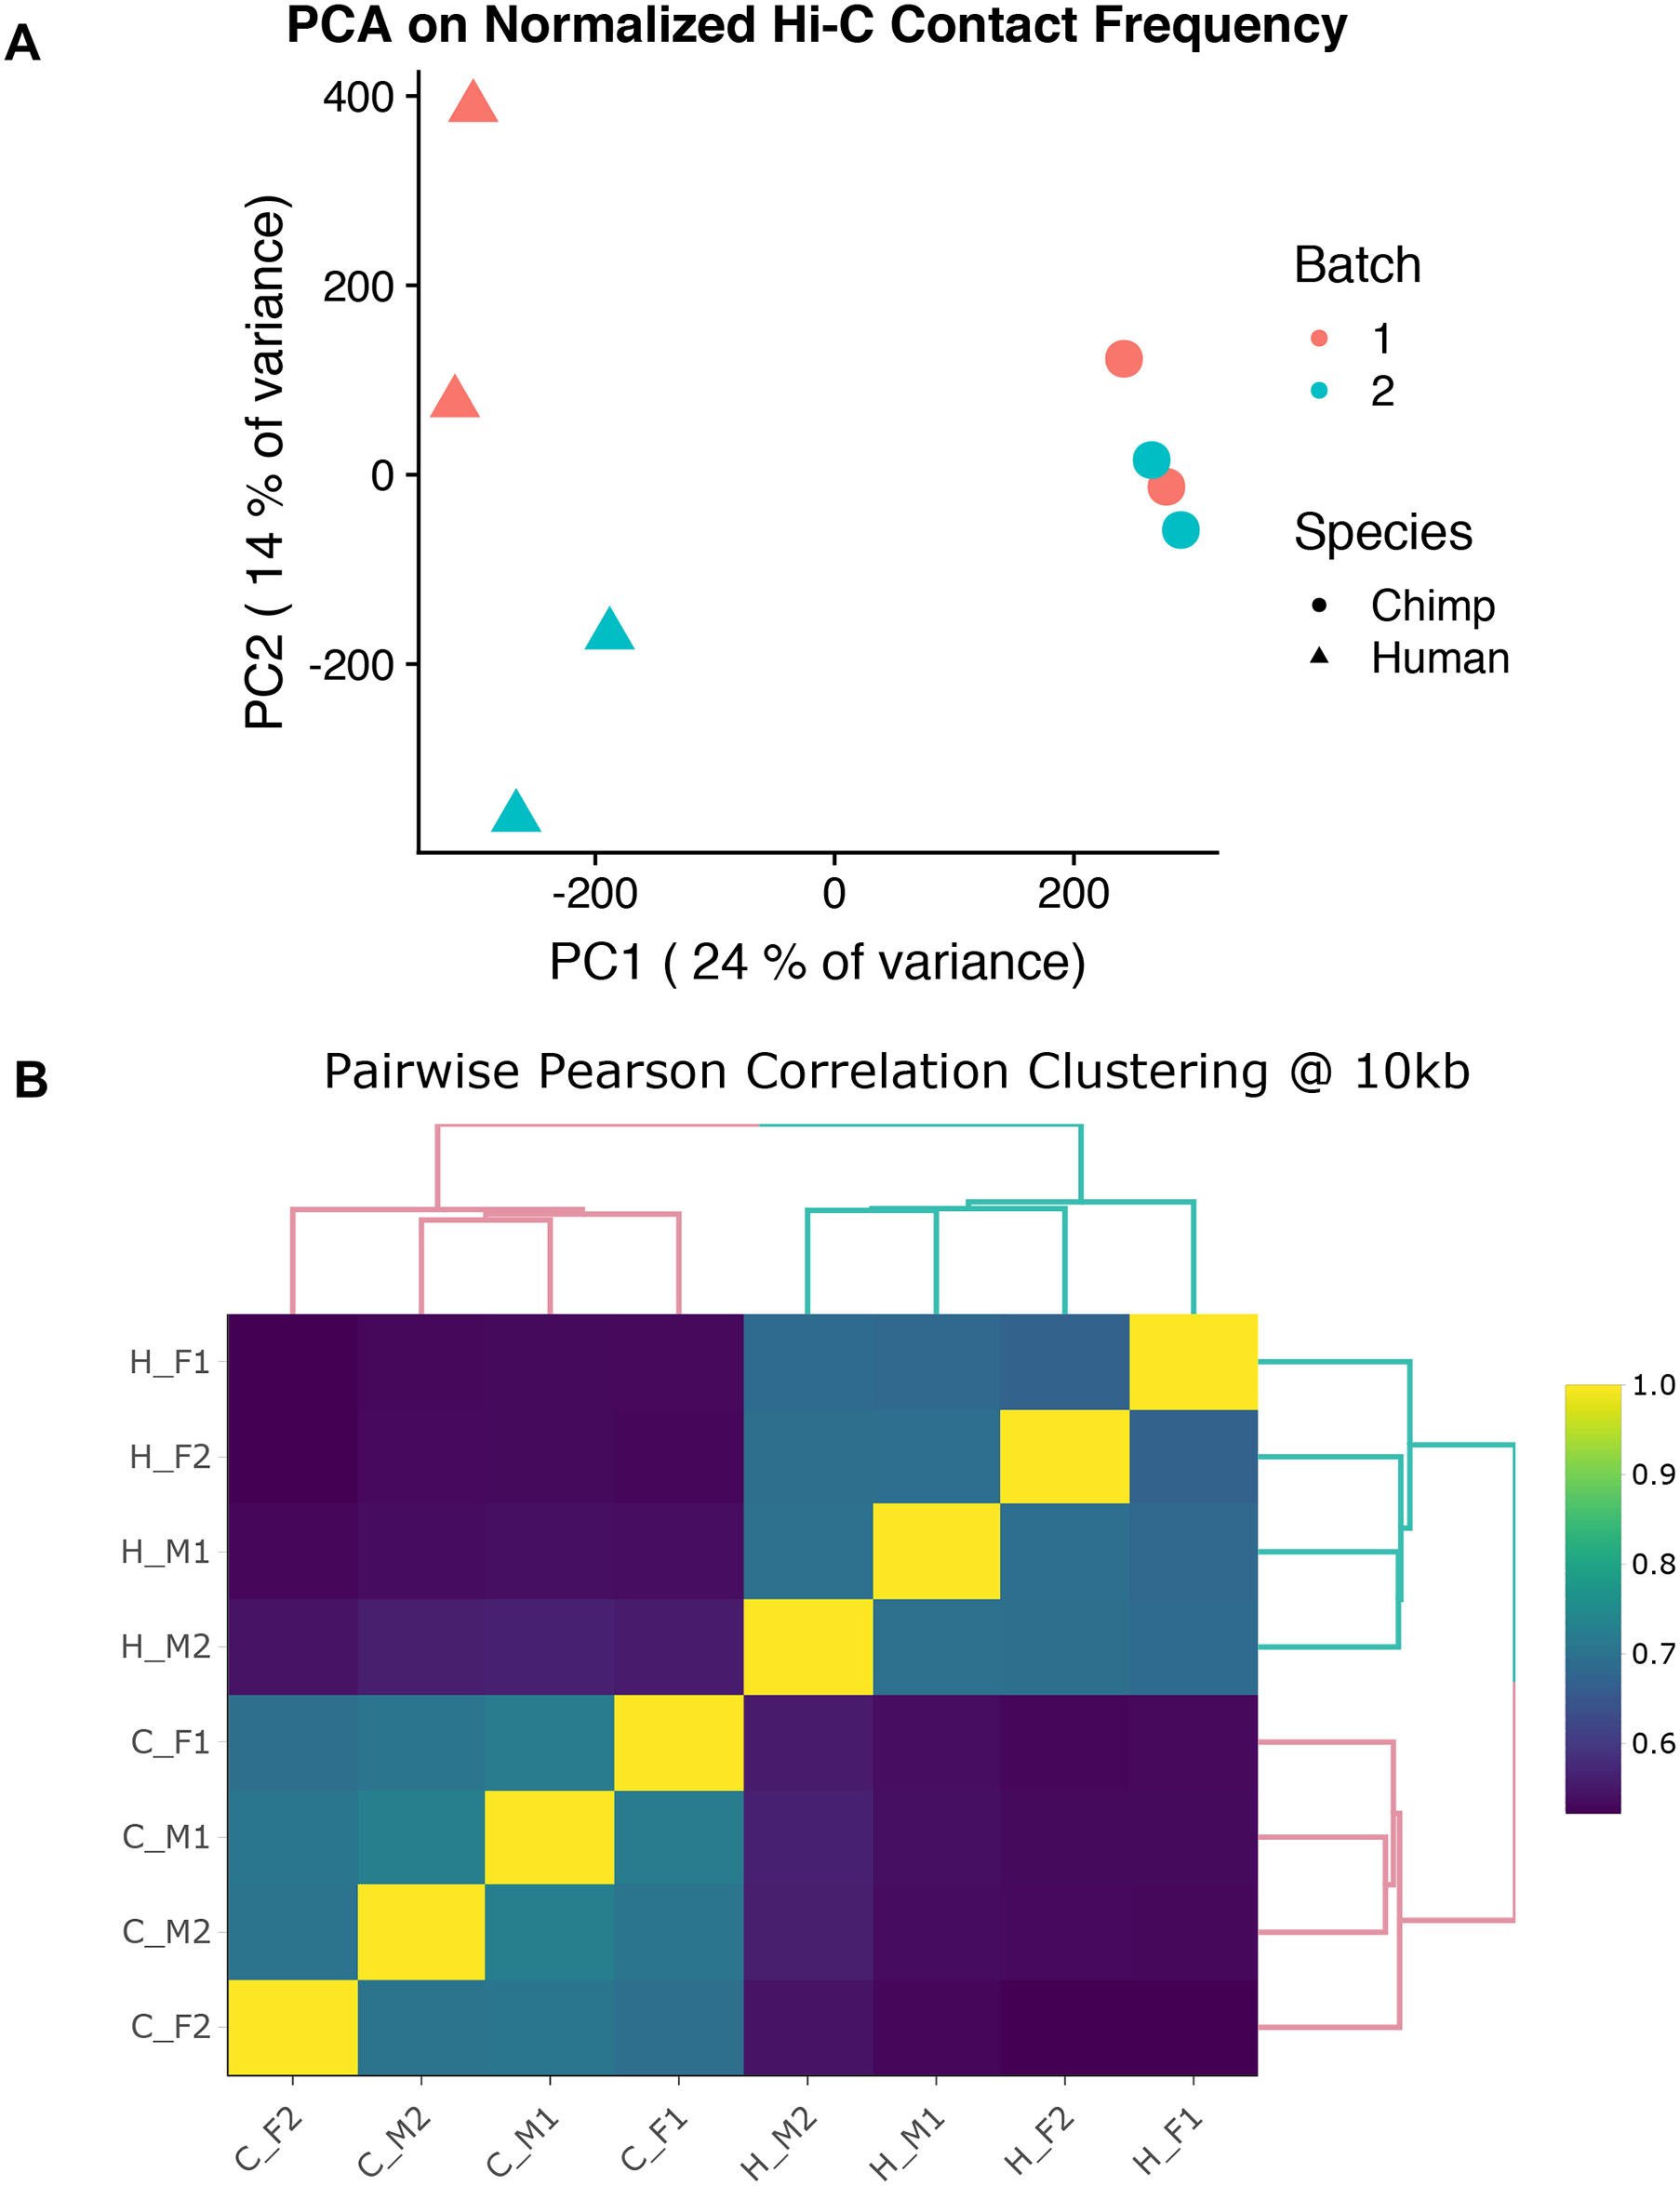
\includegraphics[width=4in]{img/fig1.PNG}
\caption[General patterns in Hi-C data.]{\textbf{General patterns in Hi-C data.} (A) Principal components analysis (PCA) of HOMER-normalized interaction frequencies for the union of all contacts in humans (triangles) and chimpanzees (circles). PC1 is highly correlated with species (r = 0.98; P {\textless} 10\textsuperscript{-5}). (B) Unsupervised hierarchical clustering of the pairwise correlations (Pearson's r\textsuperscript{2}) of HOMER-normalized interaction frequencies at 10 kb resolution. The first letter in the labels demarcates the species (H for human and C for chimpanzee), and the following symbols indicate sex (male, M or female, F) and batch (1 or 2).}
\label{fig:ch02-fig1}
\end{figure}

To identify inter-species differences in contact frequencies, we analyzed the data using a linear model with fixed effects for species, sex, and processing batch (see Methods). At an FDR of 5\%, we classified 13,572 contacts (about 4\%) as having differential normalized contact frequency between humans and chimpanzees. Analysis of the orthologous regions anchoring these contacts suggested that approximately 4,000 of these differences might be explained by large inter-species differences in distance between mates of a contact pair (because read count is correlated with distance between the mates; see Methods and S9 Fig). We thus conservatively excluded locus pairs whose distance varied by more than 20 kb across species. Ultimately, we classified with confidence 9,661 Hi-C contacts (of 292,070; about 3.3\%) with a significant difference in normalized contact frequency between the two species. We refer to these contacts as inter-species differentially contacting (DC) regions (S10 Table). Our observations thus suggest that lower-order contacts are generally conserved between humans and chimpanzees. That said, if we assume that all of the contacts we filtered out (either due to lack of orthology or because the distance between the anchor regions differed across species) are in fact DC, divergence in contact frequency would have been observed for 16\% of the Hi-C contacts (assuming similar properties to the current data set). However, we find it more likely that a large subset of the contacts we excluded are not truly DC, but, rather, not comparable between the species due to differences in genome assembly quality.

Across all DC regions, 55\% exhibited a higher contact frequency in chimpanzees, while 45\% showed a higher frequency in humans (Fig 2A, see Fig 3 and S10 Fig for examples). We observed that some chromosomes were associated with greater asymmetry in inter-species contact frequencies than others (Fig 2B). Greater asymmetry seems to be present more often in chromosomes with large inter-species rearrangements. Specifically, in our data, 8 of the 9 chromosomes with known large-scale pericentric inversions between the species (1, 4, 5, 9, 12, 15, 16, 17, and 18; \cite{Yunis.1982, Yunis.1980, Kehrer-Sawatzki.2005, Nickerson.1998, Waterson.2005, Dennehey.2004}) show particularly strong asymmetry in inter-species contact frequencies. We also observed asymmetry in inter-species contact frequencies in human chromosome 2, a fusion of the ancestral chromosomes giving rise to chimpanzee chromosomes 2A and 2B \cite{Waterson.2005}, as well as in chromosome 7, which has the highest number of un-localized sequences of any chromosome in the panTro5 genome.

\begin{figure}
\centering
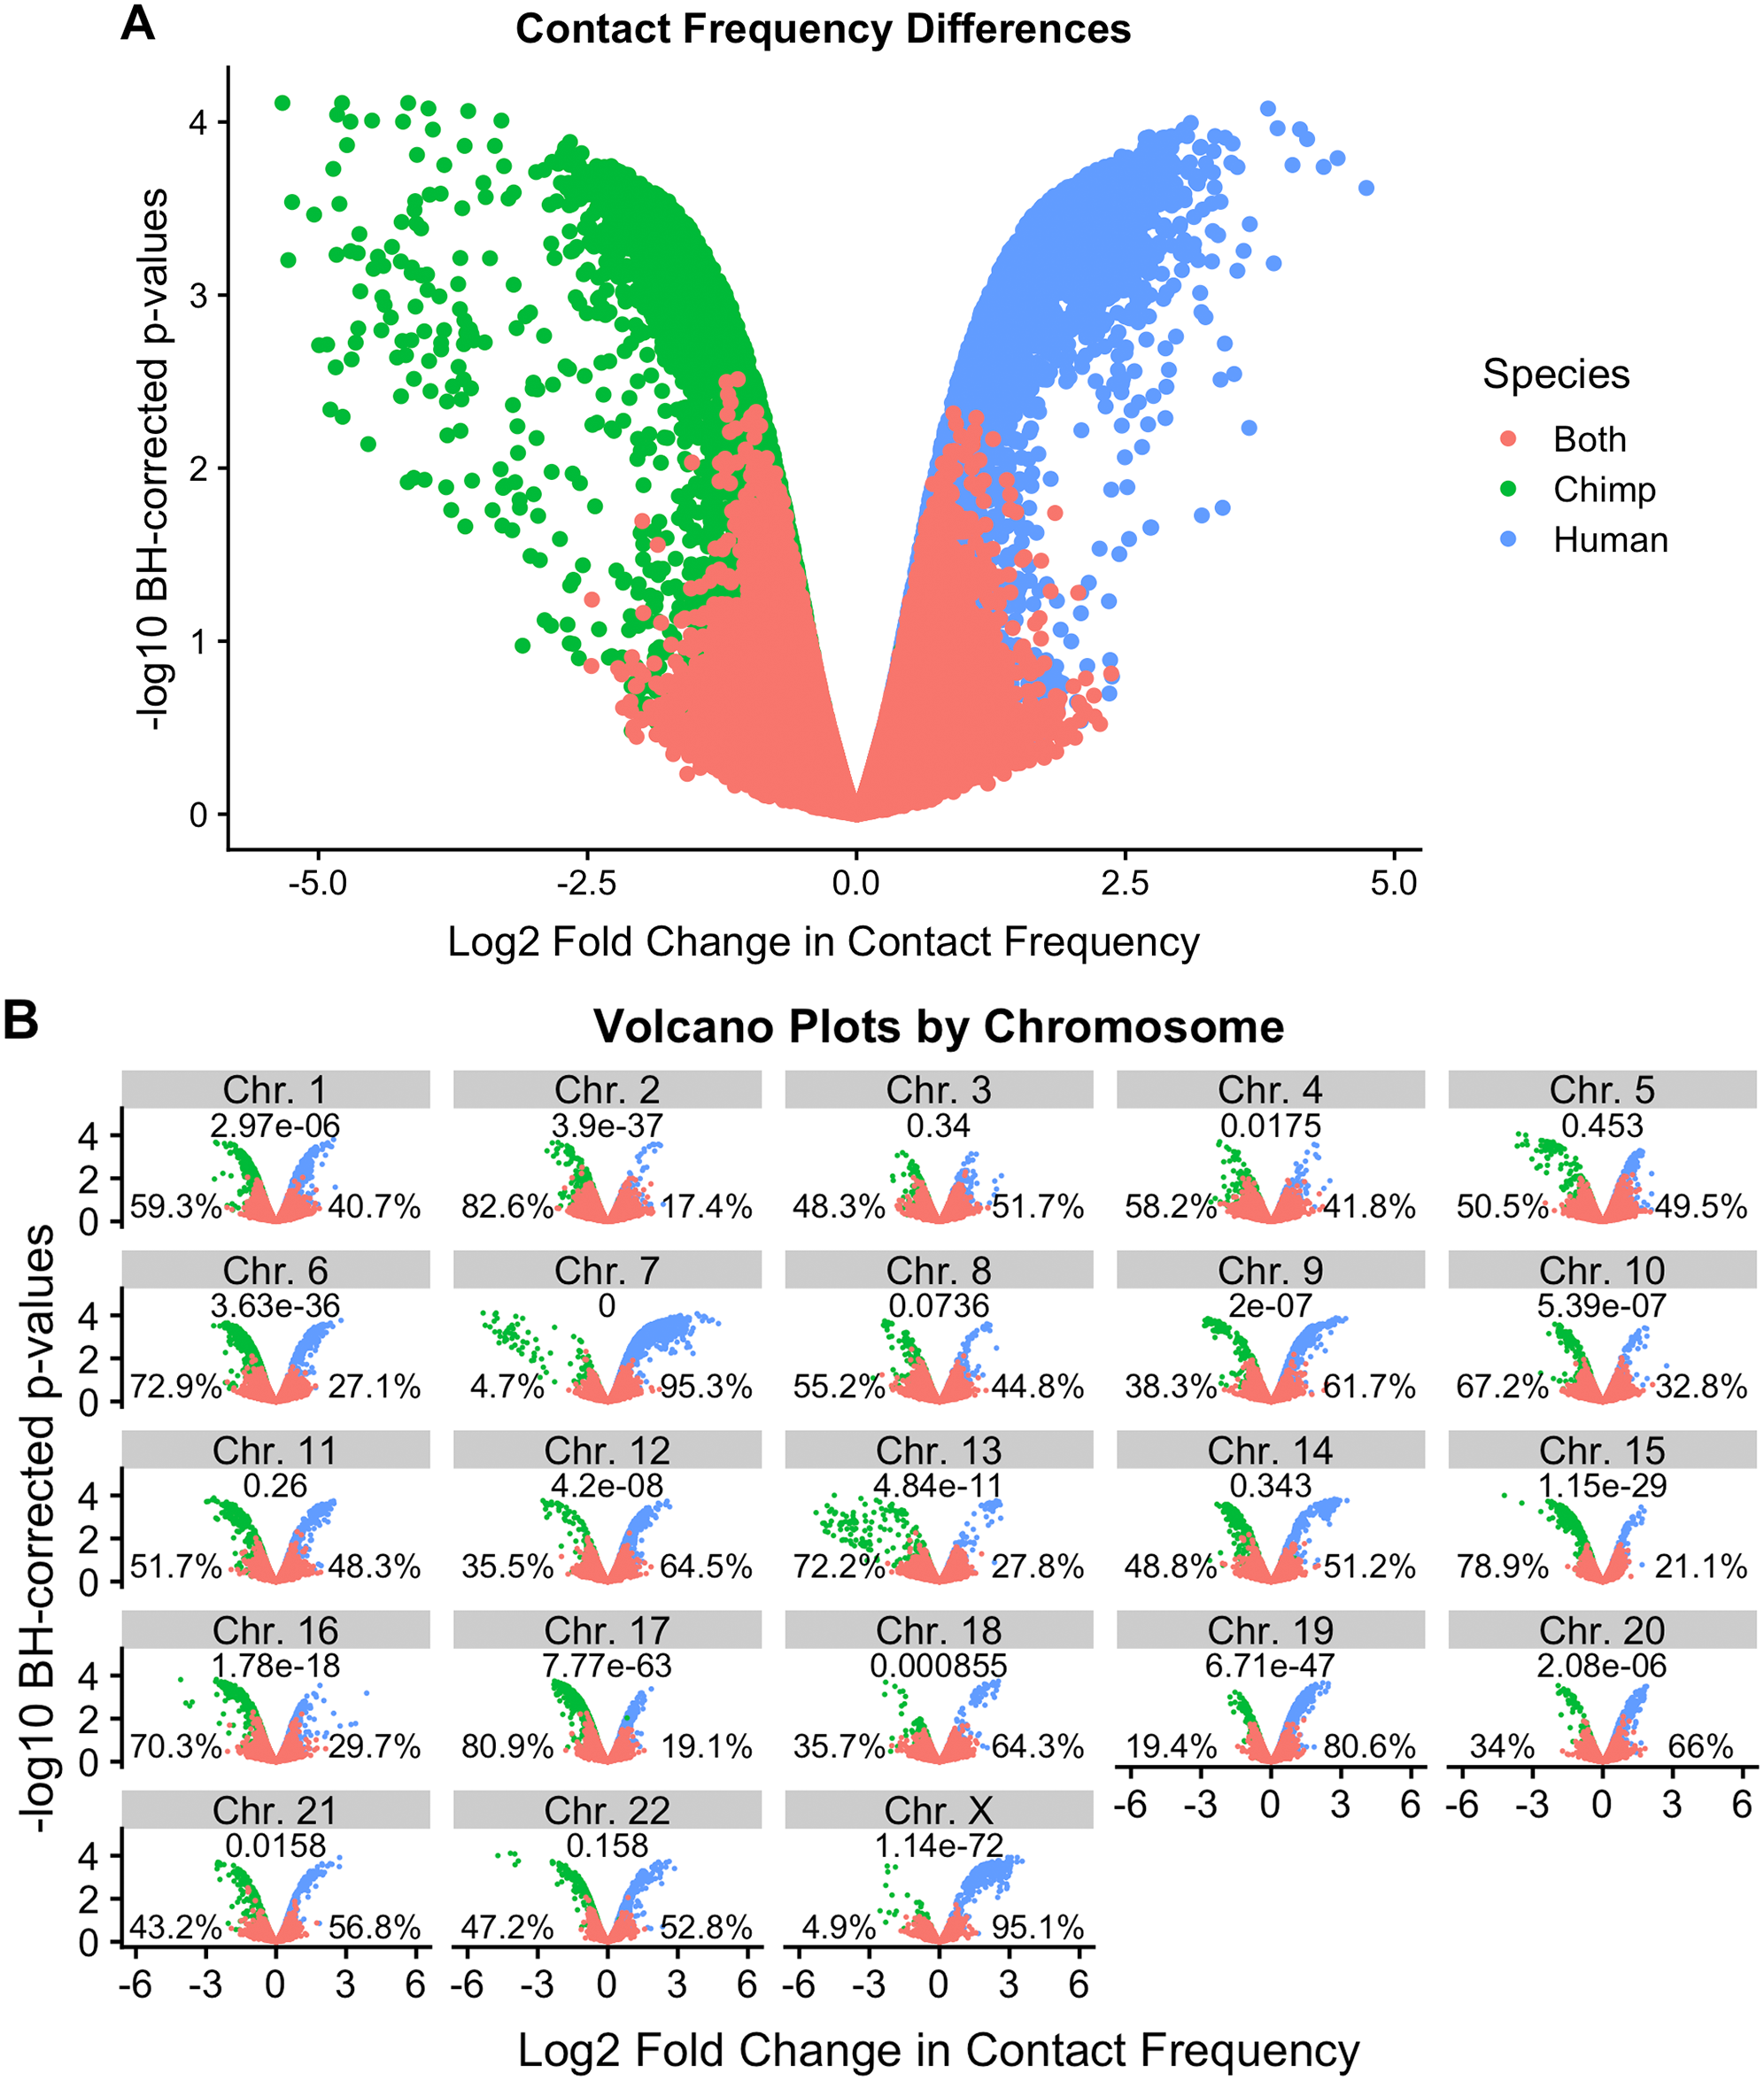
\includegraphics[width=6in]{img/fig2.PNG}
\caption[Linear modeling reveals large-scale chromosomal differences in contact frequency.]{\textbf{Linear modeling reveals large-scale chromosomal differences in contact frequency.} (A) Volcano plot of log\textsubscript{2} fold change in contact frequency between humans and chimpanzees (x-axis) against Benjamini-Hochberg FDR (y-axis), after filtering non-orthologus regions (results for unfiltered data are plotted in S9 Fig). Data are colored by the species in which the contact was originally identified as significant. (B) Per-chromosome volcano plot using the same legend as in A. P-values provided for a binomial test of the null that inter-species differences in contact frequencies are evenly distributed. The percentage of contacts with significant higher frequency in each species is noted.}
\label{fig:ch02-fig2}
\end{figure}

\begin{figure}
\centering
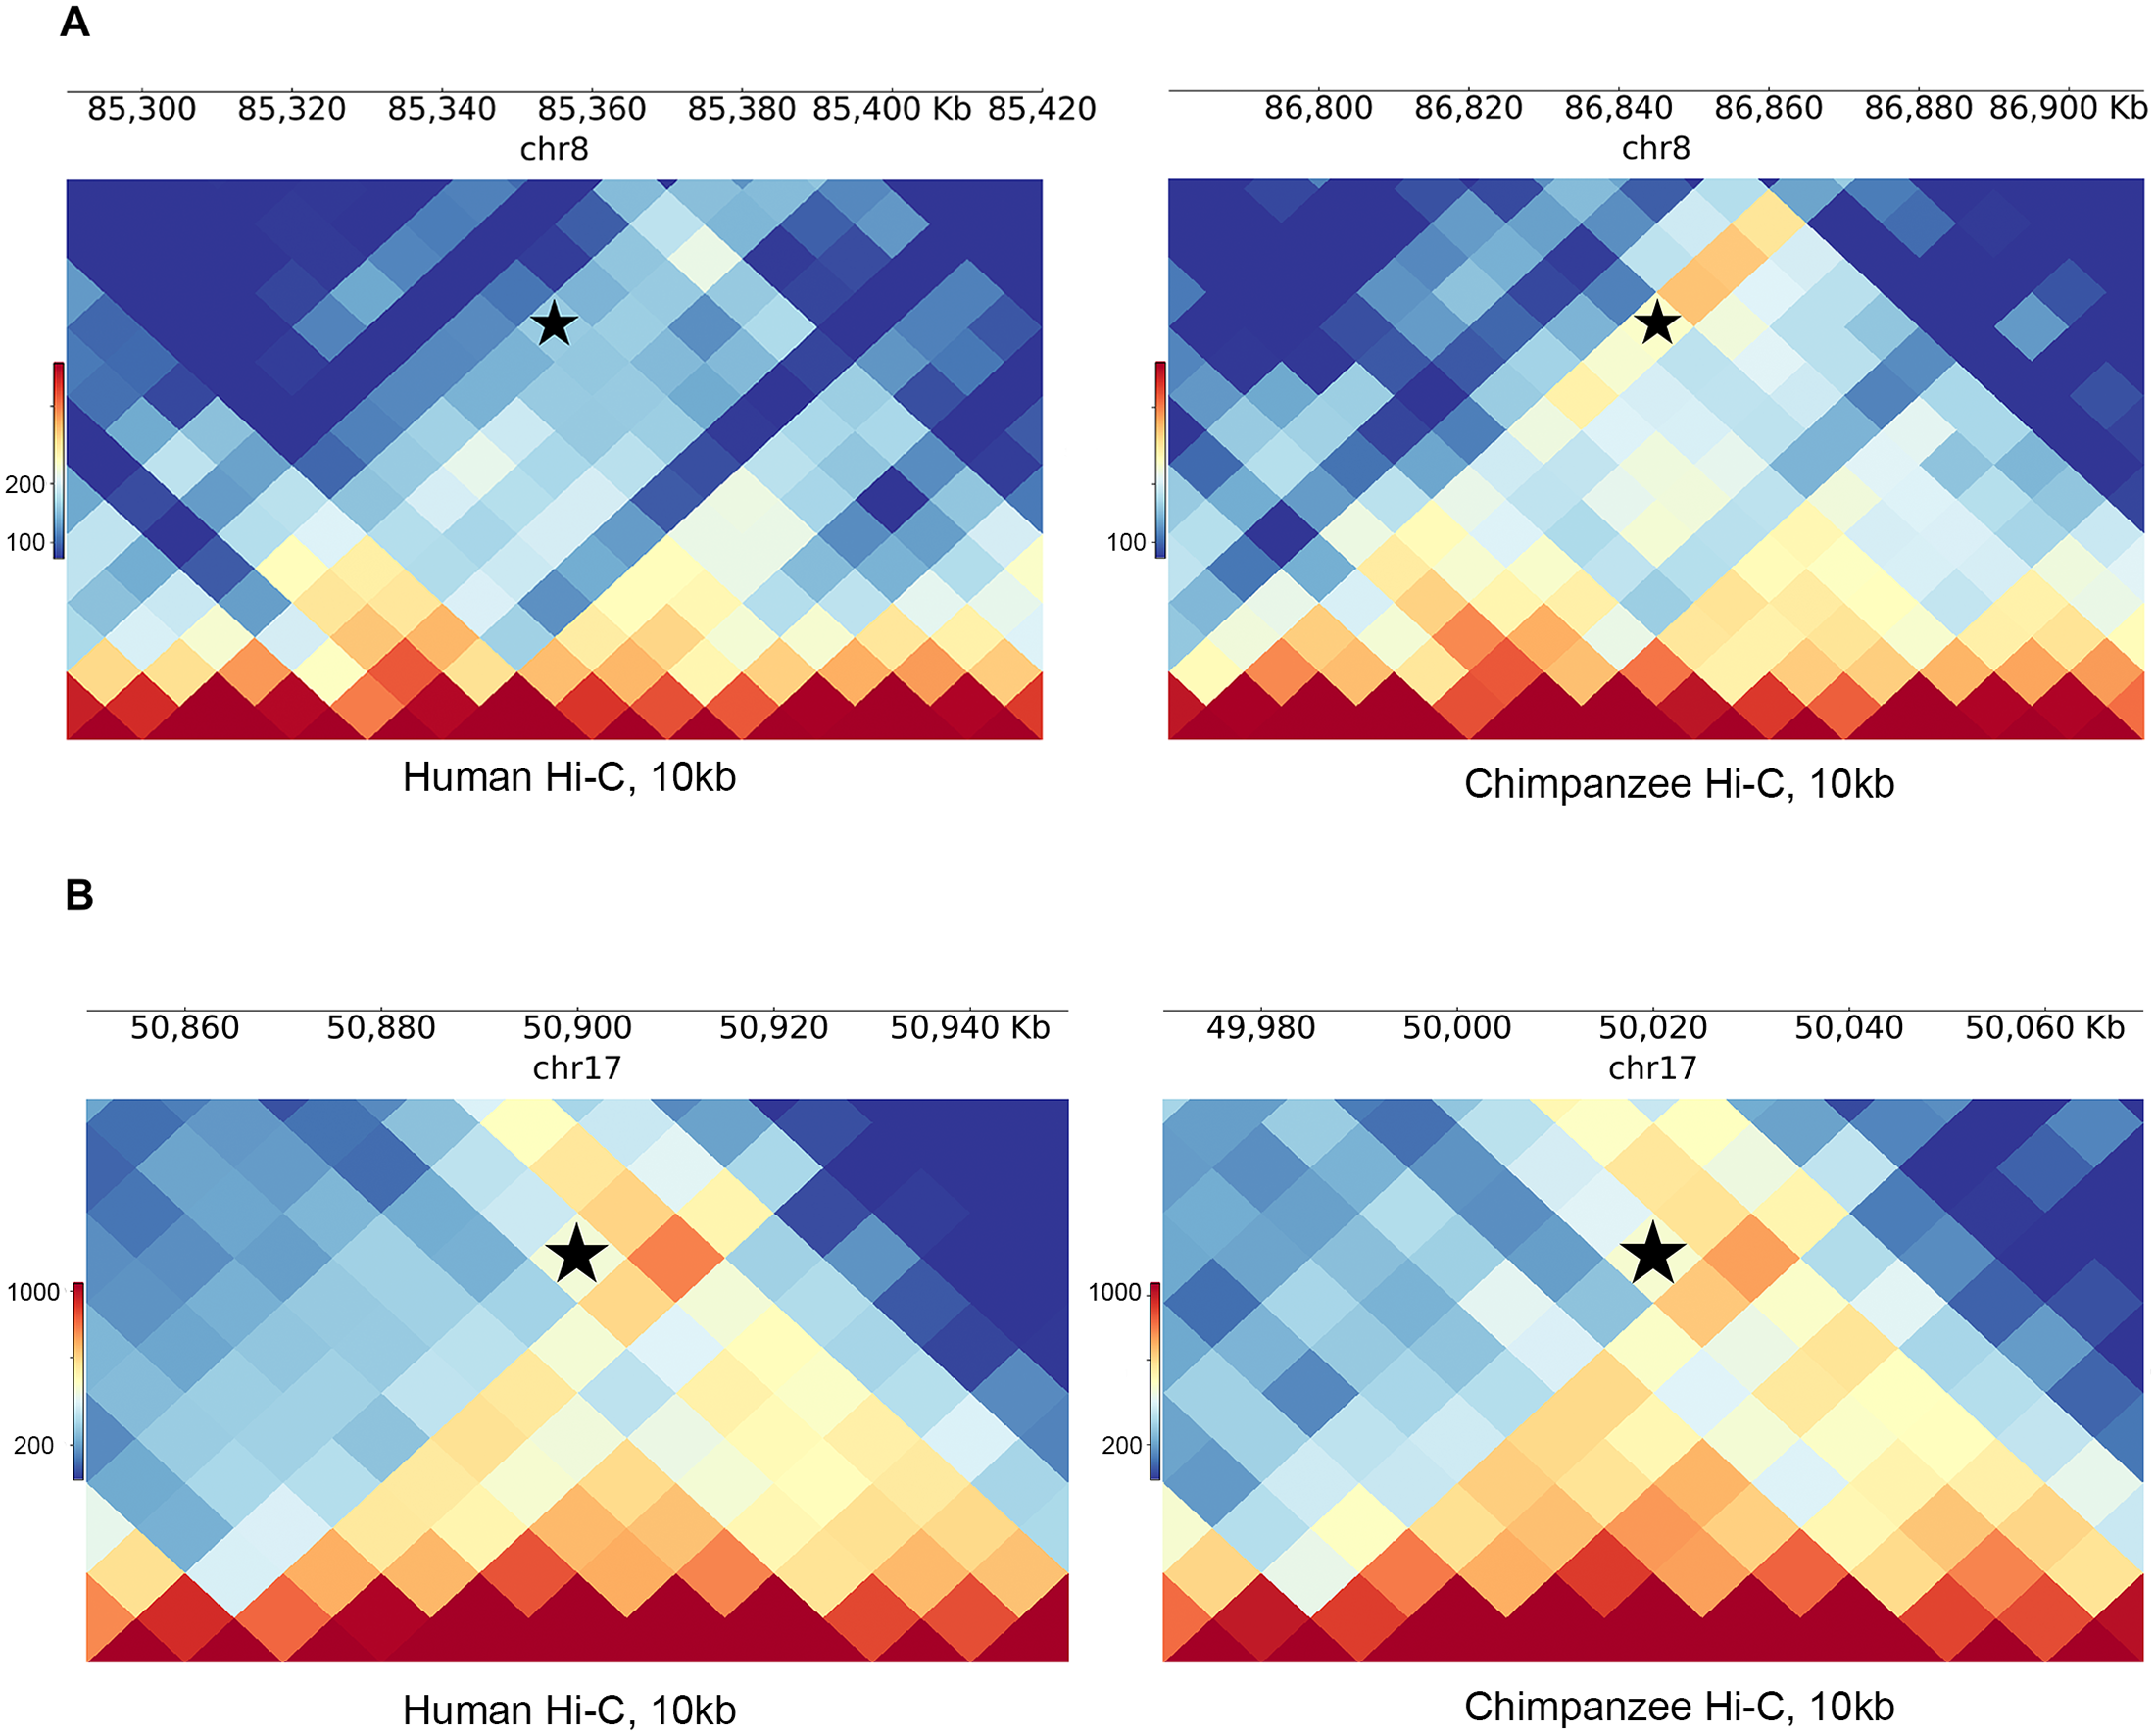
\includegraphics[width=6in]{img/fig3.PNG}
\caption[Examples of DC and non-DC Interactions.]{\textbf{Examples of DC and non-DC Interactions.} (A) PyGenomeTracks plots \cite{Ramirez.2018} of a chromosome 8 interaction between bins 130kb away for human (left panel) and chimpanzee (right). The bin pair tested is indicated by a black star, and was found to be DC between species. (B) Same as A, but for a conserved (non-DC) interaction on chromosome 17 separated by 100kb.}
\label{fig:ch02-fig3}
\end{figure}

Next, we turned our attention to higher-order chromosomal structures by characterizing TADs in each species. Previous studies indicate that the human and chimpanzee genomes share a high degree of synteny \cite{Yunis.1982, Yunis.1980, Scally.2012, Kehrer-sawatzki.2007, Catacchio.2018, Lee.2016}, a property we confirmed by tiling each genome into various bin sizes and using a reciprocal best hits liftOver method to identify syntenic regions (see Methods and S11 Fig). To infer steady-state TAD structures, we pooled reads across all individuals within each species to create `high-density consensus' Hi-C maps for humans and chimpanzees \cite{Durand.2016}. We used the Arrowhead algorithm at 10 kb resolution \cite{Durand.2016} to independently infer 11,298 TADs in humans and 10,505 TADs in chimpanzees (see Methods). We then used liftOver to identify orthologous genomic regions that corresponded to these TADs, and removed 10\% of domains for which orthology could not be identified (S11 and S12 Tables list the TADs identified in each species; S13 Table lists the orthologous locations of the combined TADs). Once orthology has been established, for each TAD, we considered the domain conserved in humans and chimpanzees when 90\% of the TAD interval overlapped reciprocally between species (see Methods). Using this approach, we found that only $\sim$43\% of TADs discovered in humans and chimpanzees are shared (Fig 4A).

\begin{figure}
\centering
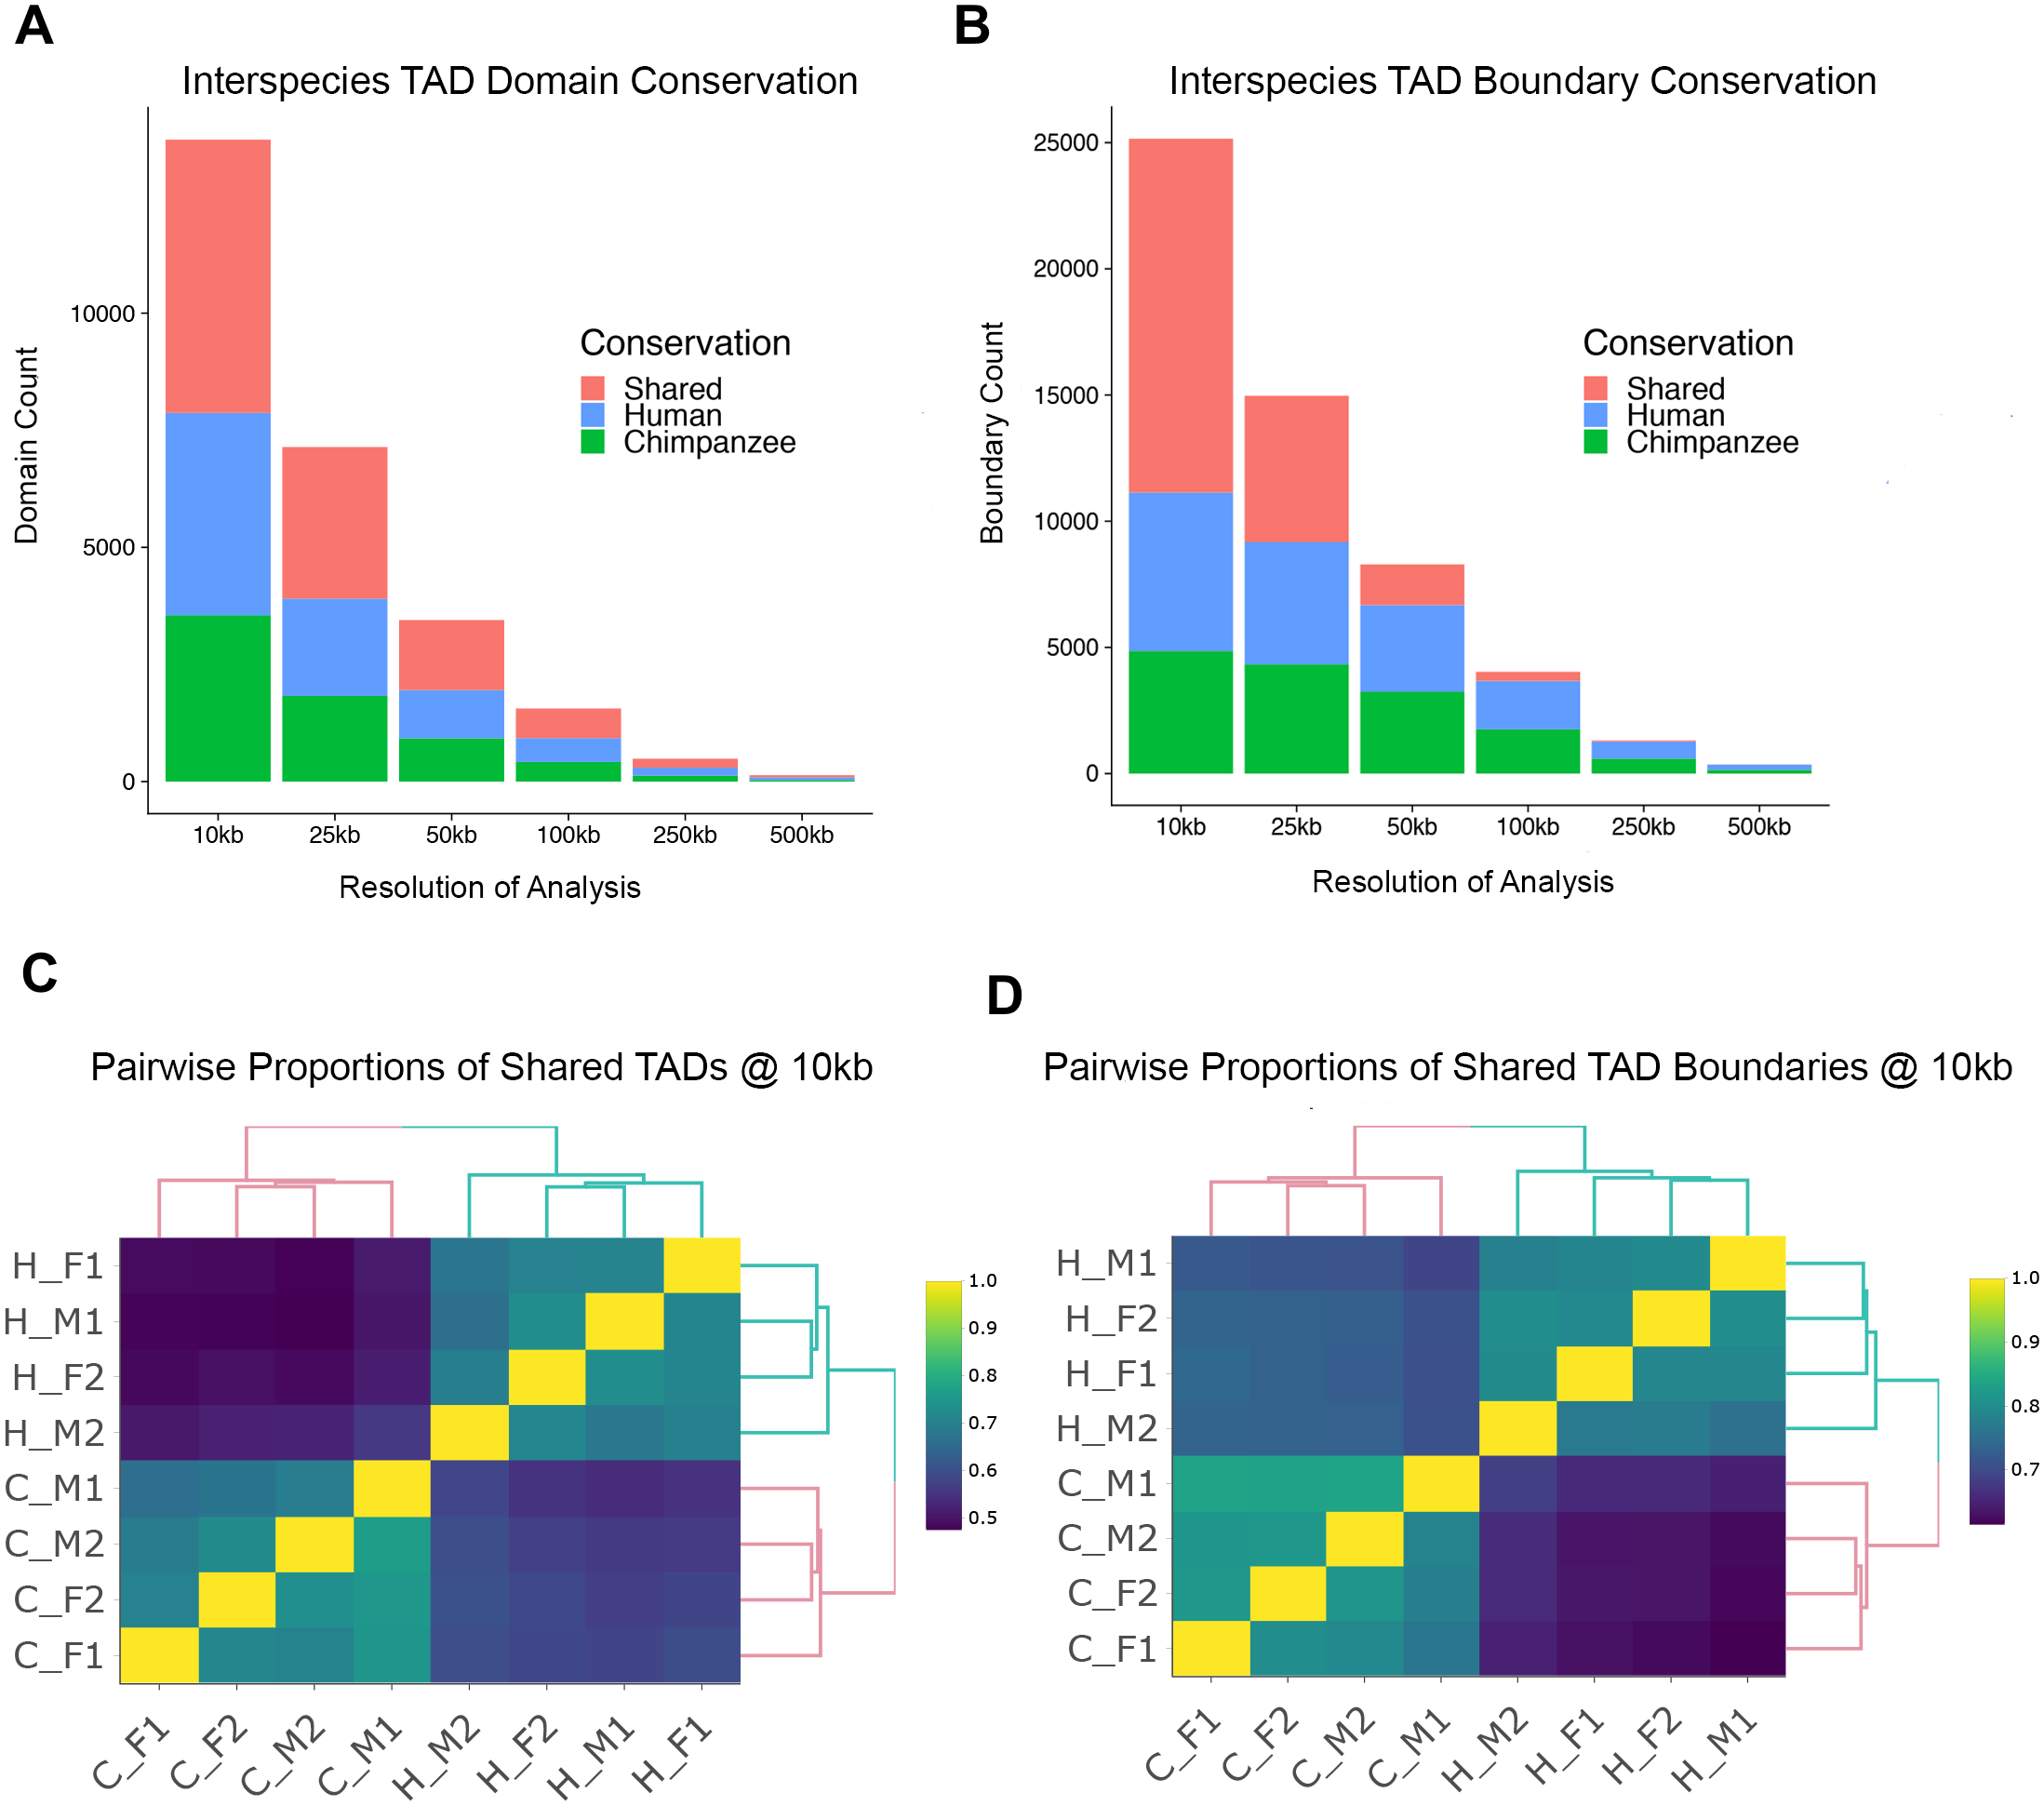
\includegraphics[width=6in]{img/fig4.PNG}
\caption[Higher-order chromosomal structure in humans and chimpanzees.]{\textbf{Higher-order chromosomal structure in humans and chimpanzees.} (A) Across different resolutions (x-axis), we plotted the number of shared and species-specific domains (y-axis) identified with Arrowhead \cite{Durand.2016} using the consensus map from each species (alternative approaches plotted in S12{\textendash}S14 Figs). (B) Same as A, but for TAD boundaries instead of the domains themselves. Boundaries were defined as 15kb flanking regions at the edges of inferred Arrowhead domains. (C) Unsupervised hierarchical clustering of pairwise comparison of TADs across all individuals. These proportions were obtained using Arrowhead TAD inferences on each individual at 10kb resolution. Proportions indicated by color scale on right. Similar plots using analysis at different resolution are available in S12 and S14 Figs. (D) Similar to C, but for TAD boundaries instead of the domains themselves.}
\label{fig:ch02-fig4}
\end{figure}

The observation that TADs are generally not as conserved as practically all other regulatory phenotypes studied in humans and chimpanzees was unexpected. We thus thoroughly tested the robustness of this inference. To do so, we performed a large number of alternative analyses. We analyzed the data at different resolutions (from 10 kb to 500 kb---each time repeating the reciprocal liftOver analysis). We analyzed the data by considering, instead of pooled data, TADs identified independently in a single and in up to 4 individuals within each species (Fig 4C and S12 Fig), and we did this across the different resolutions. We analyzed the data by classifying conservation based on the approach of Rao et al. \cite{Rao.2014} instead of relying on an overlap of 90\% of the domain; we analyzed the pooled data using panTro6 as a reference genome rather than the panTro5 assembly (S13 Fig). We analyzed the data by focusing on boundaries instead of the entire domains (Fig 4B and 4D); we used multiple alternative definitions of boundaries, and repeated this analysis across all resolutions and with boundaries identified in different numbers of individuals within species (S12 Fig). Finally, we identified TADs using an alternative algorithm, TopDom \cite{Shin.2016}, and repeated all of the alternative analyses mentioned above using this algorithm (S14 Fig).

The results of many of these alternative analyses are reported in the supplement (S10 and S12{\textendash}S14 Figs). All of the alternative analyses produced consistent results and an inference that TADs and TAD boundaries are much less conserved between humans and chimpanzees than any other regulatory phenotype studied to date \cite{Pai.2011, Shulha.2012, Calarco.2007, Trizzino.2017, Prescott.2015, Kim.2011}. The Arrowhead analysis of TADs that are independently identified in four individuals within either species, at 10 kb resolution, where conservation is classified based on the less stringent approach of Rao et al. \cite{Rao.2014}, resulted in the highest estimate of conservation, with 78\% of domains and 83\% of boundaries shared between the species (S12B and S12D Fig). The restriction to TADs or boundaries identified in all 4 individuals of either species results in far fewer features that can be examined (S12 and S14 Figs), yet even in this analysis conservation of domains and boundaries is modest (see Fig 5 and S10 Fig for examples).

\begin{figure}
\centering
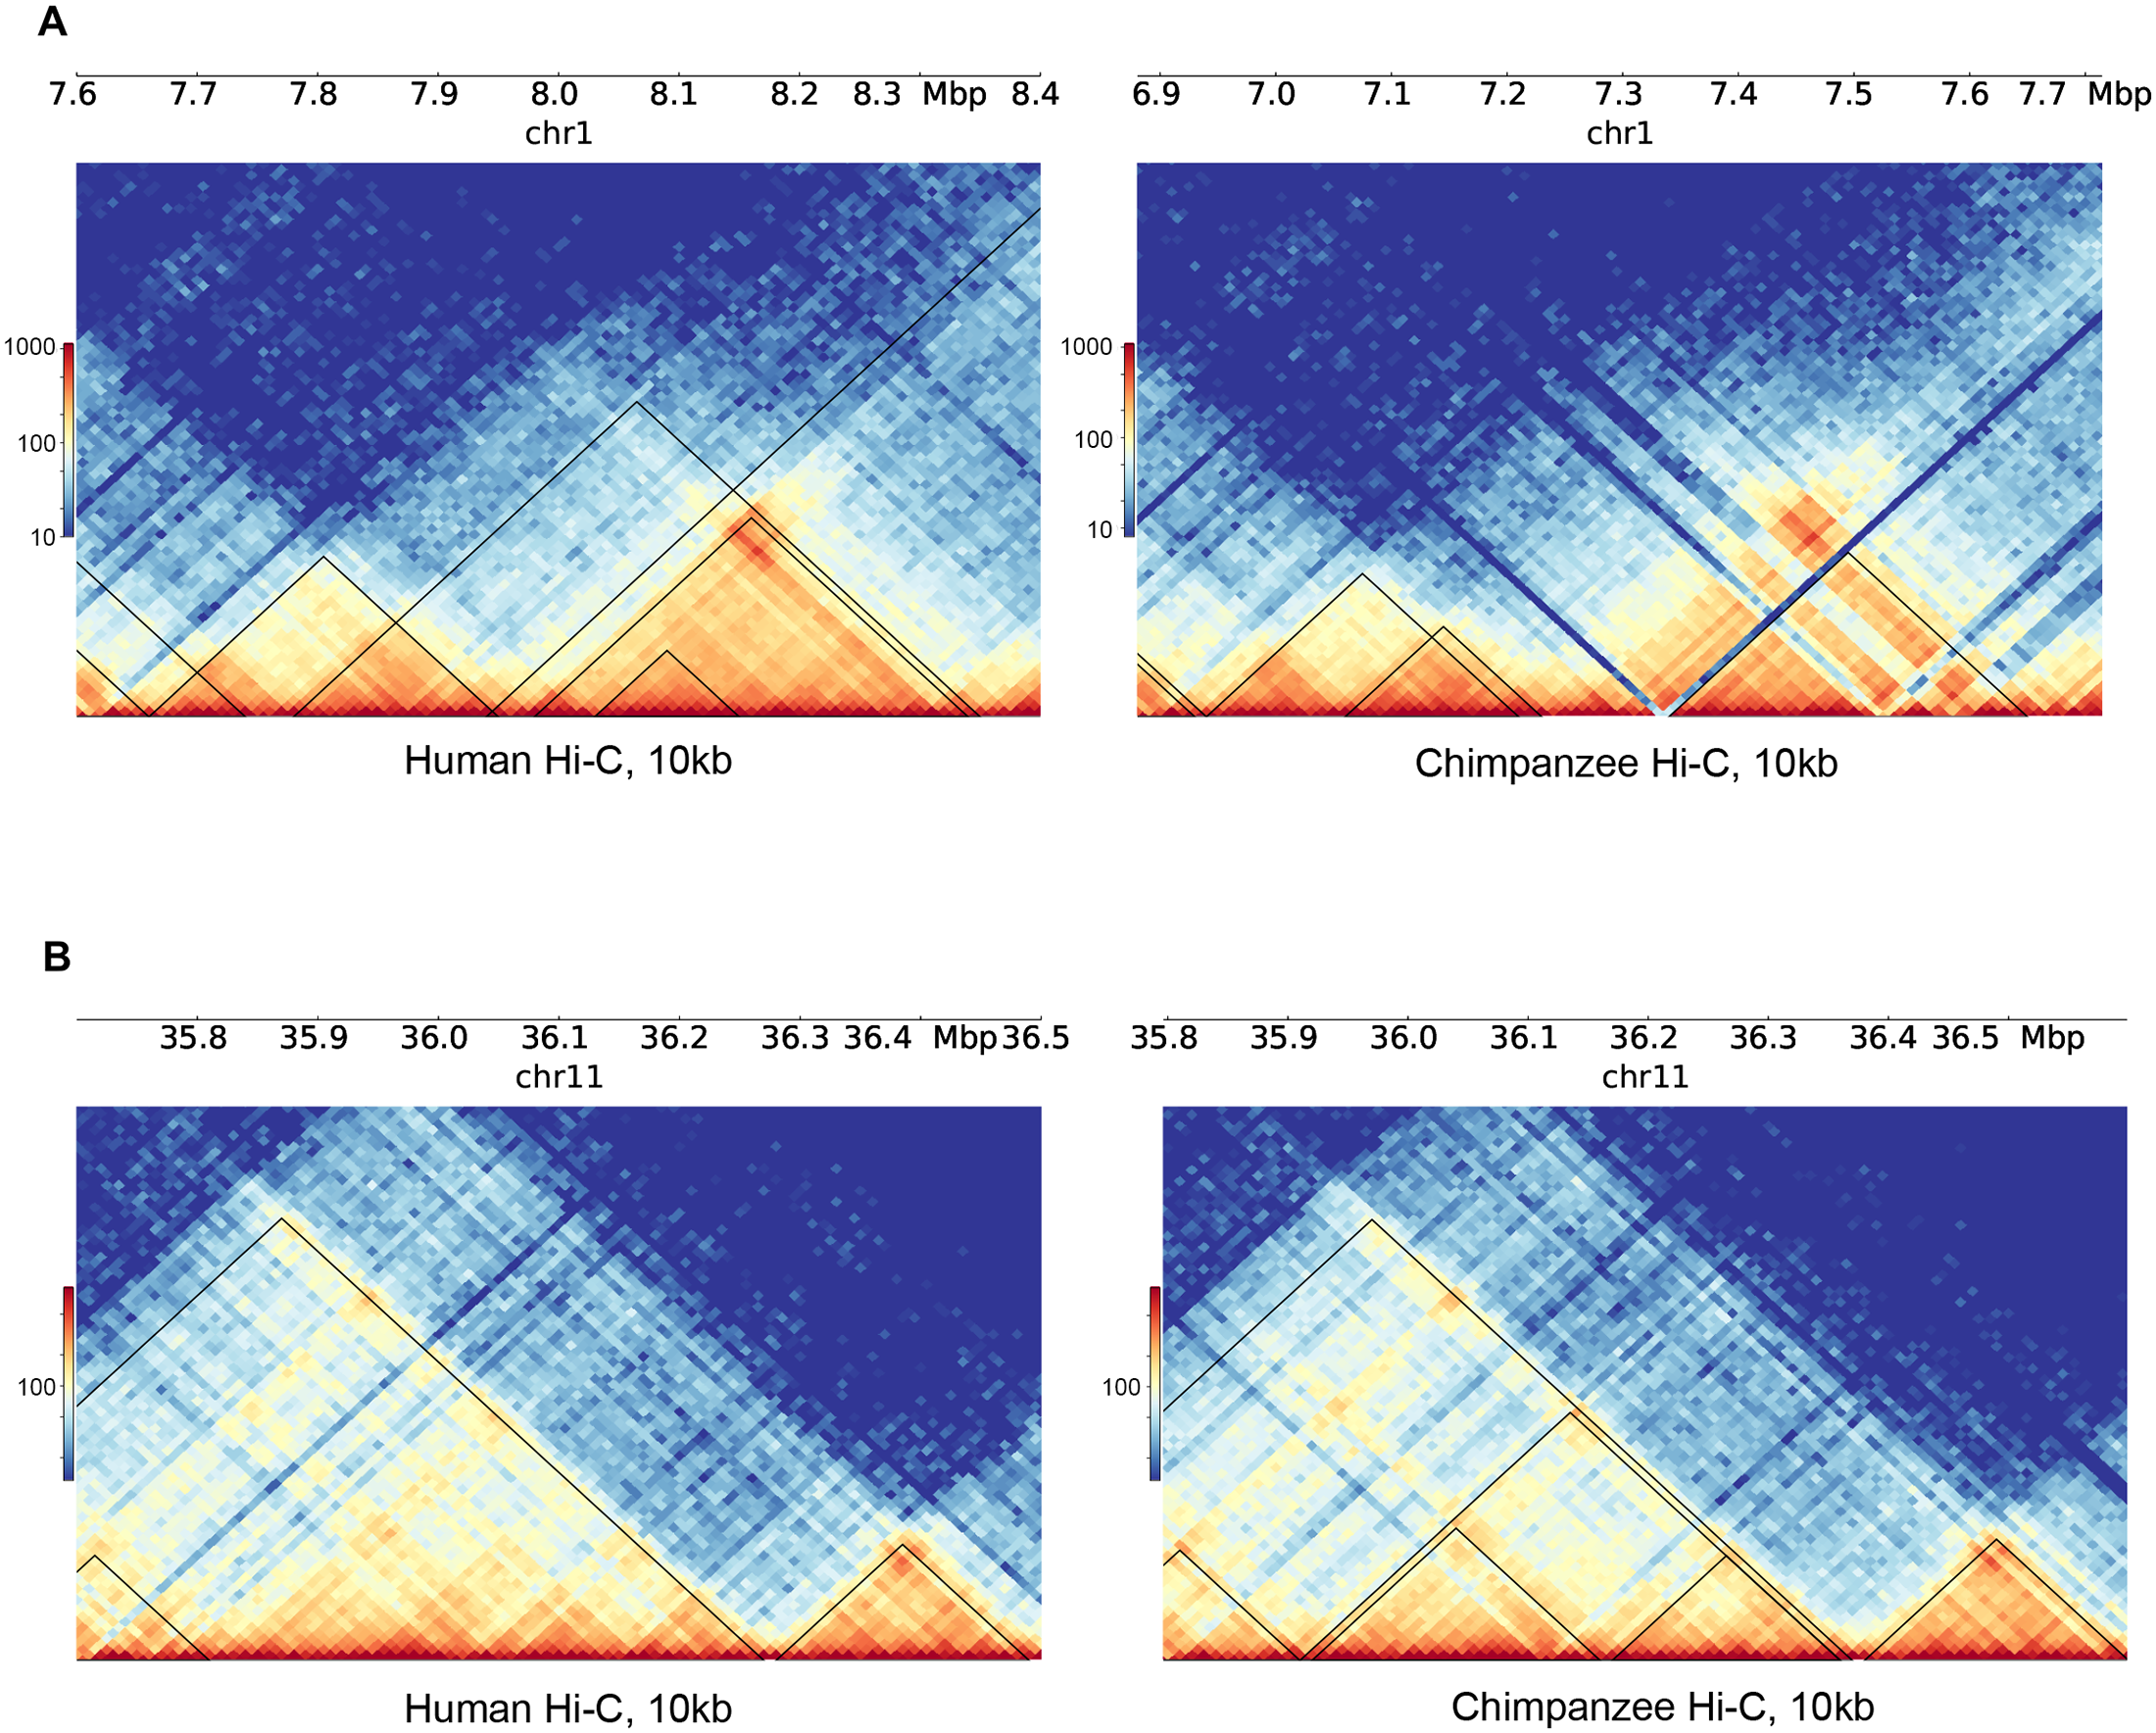
\includegraphics[width=6in]{img/fig5.PNG}
\caption[Examples of conserved and divergent TADs.]{\textbf{Examples of conserved and divergent TADs.}(A) A region on chromosome 1 with examples of both conserved and divergent Arrowhead \cite{Durand.2016} TAD inferences (black lines). Both the larger TADs seen in the chimpanzee map (right) appear to be conserved in the human map (left), whereas several of the TADs inferred in the human map are noticeably absent from the chimpanzee map. (B) A region on chromosome 11, once again showing examples of conserved and divergent Arrowhead TAD inferences (black lines). All the TADs seen in the human map (left) appear conserved in the chimpanzee map (right), whereas three smaller TADs inferred in the chimpanzee map are not found in the human map, suggesting divergence.}
\label{fig:ch02-fig5}
\end{figure}

\subsection{The relationship between inter-species differences in contacts and gene expression}

We previously collected RNA sequencing data from the same human and chimpanzee iPSC lines \cite{Pavlovic.2018}. We jointly analyzed the Hi-C and RNA-sequencing data to learn how often inter-species differences in 3D genomic contact frequencies are associated with inter-species differences in gene expression. We first identified 7,764 orthologous genes for which we have expression and Hi-C data anchored at a region that overlaps the gene's transcription start site (TSS; see Methods). A single genomic region that overlaps a TSS can have multiple contacts to other genomic regions. For the purpose of our analysis, we conservatively considered only the contact that shows the highest inter-species divergence for each gene.

We did not observe a correlation between gene expression and contact frequency when we considered data from all 7,764 genes. However, when we focused on the 1,401 genes classified as differentially expressed (DE) between humans and chimpanzees (at FDR ${\leq}$ 0.05), we observed an excess of both positive and negative correlations between inter-species differences in gene expression and inter-species differences in Hi-C contacts (S15 Fig). Indeed, genes whose TSS is associated with inter-species DC are more likely to be DE between species ($\chi^2$ test; P = 0.01; Fig 6A and 6B). The association between Hi-C contacts and gene expression divergence was somewhat stronger if instead of focusing on the contact with the highest divergence, we obtained a summary P-value \cite{Whitlock.2005} for testing the null hypothesis that there are no differences between the species in any of the contacts associated with the TSS for a given gene (P = 0.001; S20C and S20D Fig).

\begin{figure}
\centering
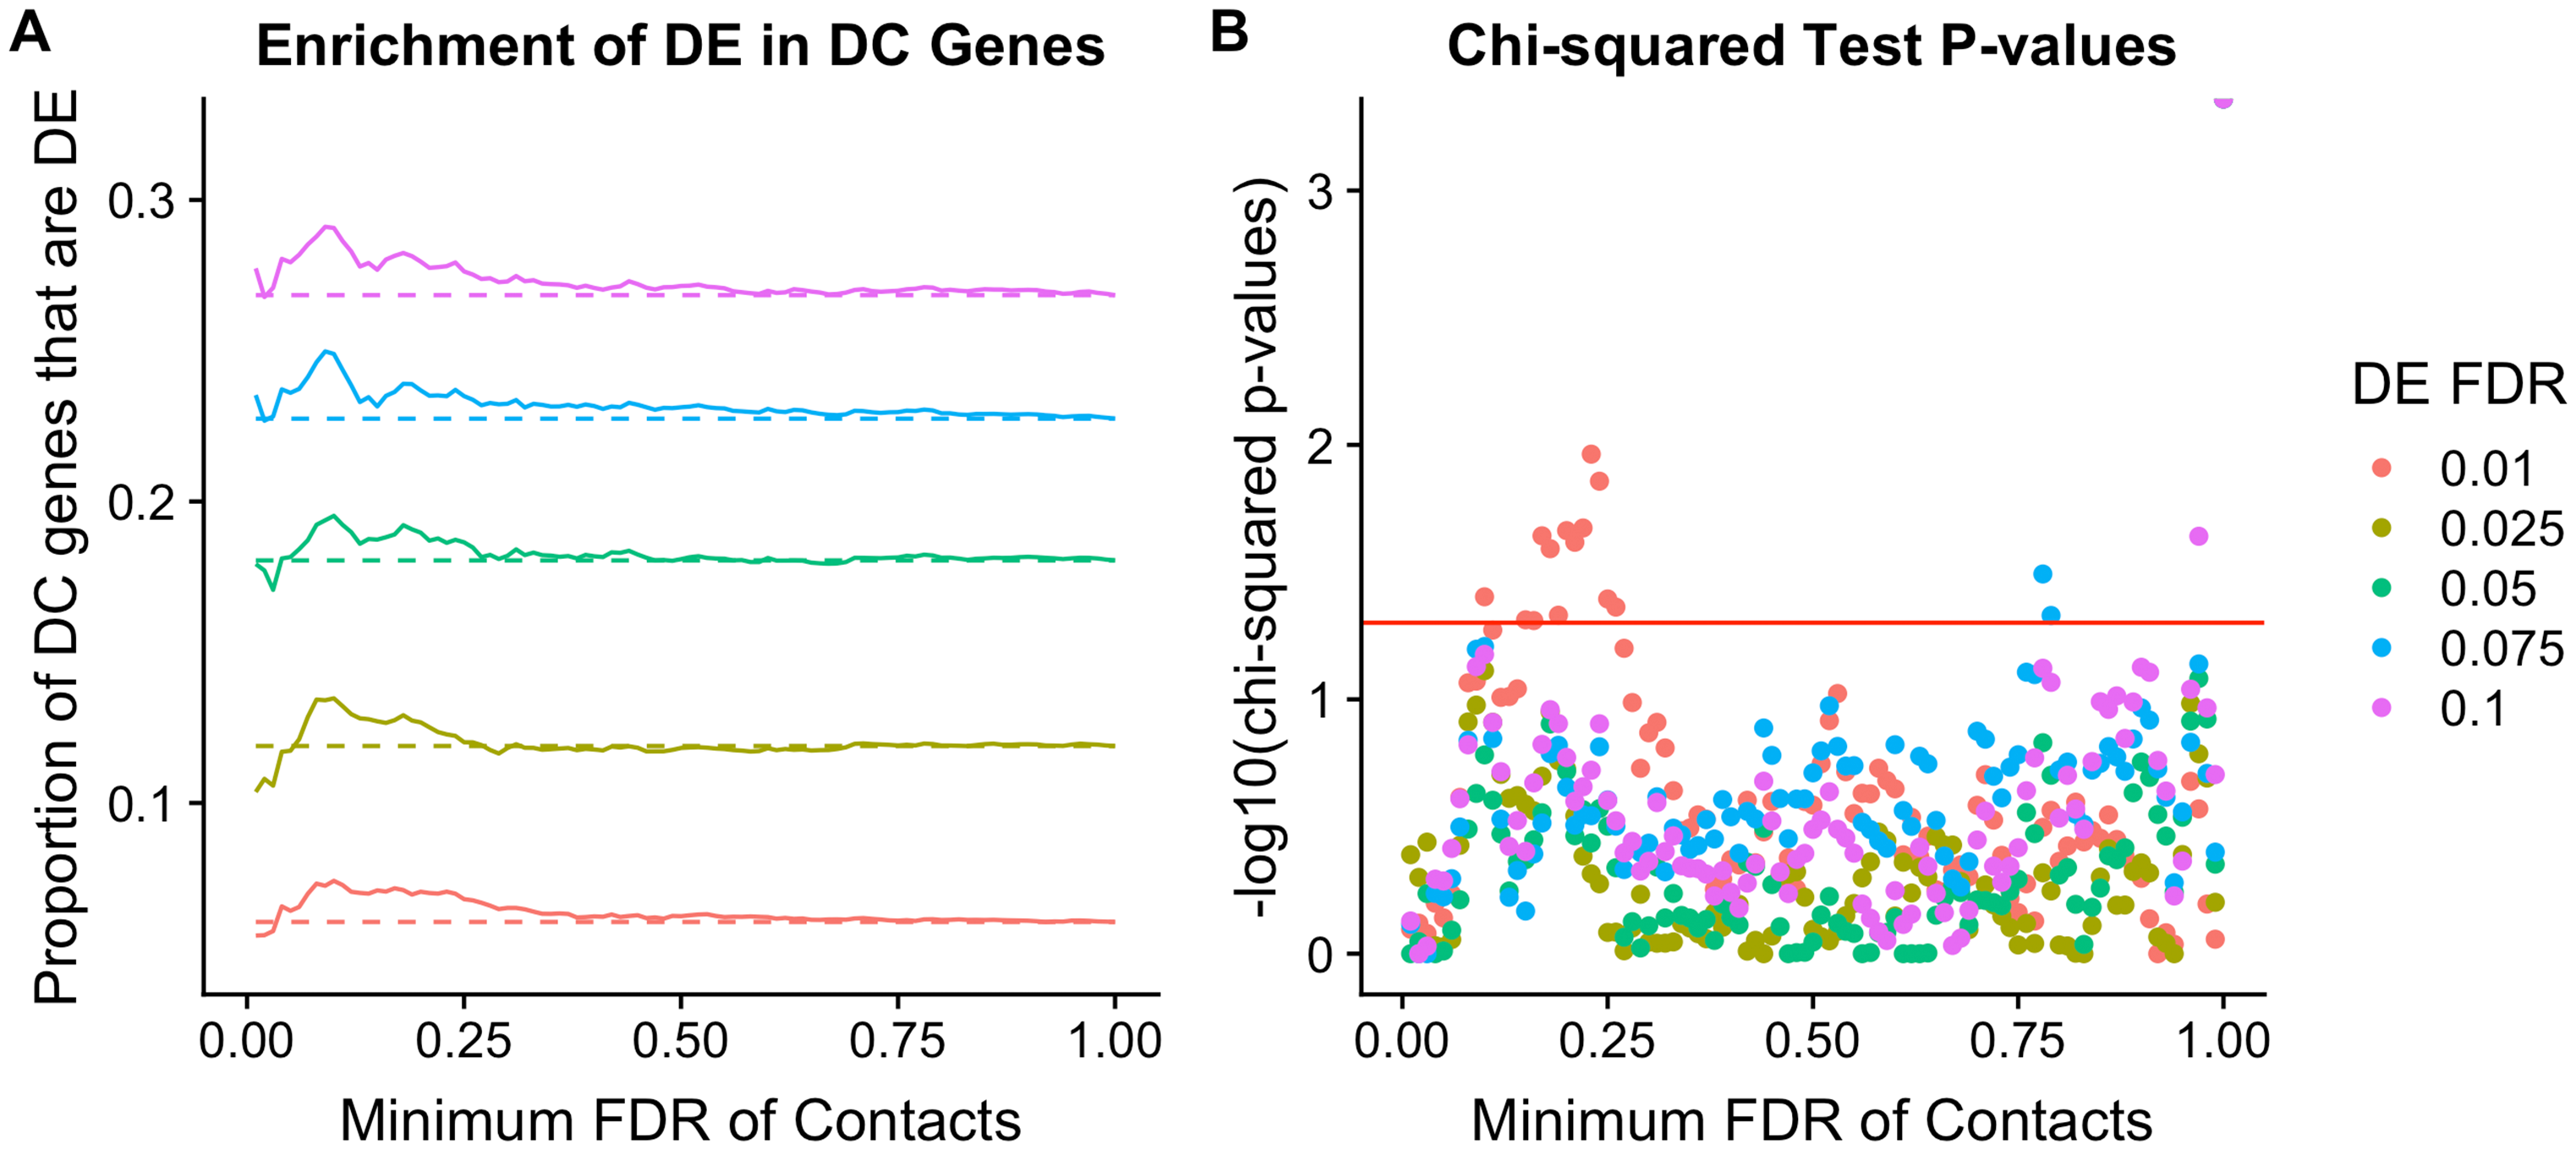
\includegraphics[width=6in]{img/fig6.PNG}
\caption[Differentially contacting Hi-C loci show enrichment for differentially expressed genes.]{\textbf{Differentially contacting Hi-C loci show enrichment for differentially expressed genes.} A) Enrichment of inter-species differentially expressed (DE) genes with corresponding differences in Hi-C contact frequencies (DC) between the species. The proportion of DC genes that are significantly DE (y-axis) is shown across a range of DC FDRs (x-axis). Colors indicate different DE FDR thresholds, and dashed lines indicate the proportion of DE genes expected by chance alone. (B) P values of Chi-squared tests of the null that there is no difference in proportion of DE genes among DC genes (y-axis), shown for a range of DC FDRs (x-axis). In both panels, DC regions were chosen to have the minimum FDR supporting inter-species difference in contact frequency. We plotted results using the weighted p-value combination instead of the minimum FDR in S20 Fig.}
\label{fig:ch02-fig6}
\end{figure}

A combined analysis of functional genomic data does not allow us to infer a direct causal relationship between chromatin contacts and gene expression patterns. Nevertheless, independent evidence strongly suggests that changes in 3D genomic structure can affect interactions between regulatory elements and promoters \cite{Rao.2014, Dily.2014, Chen.2017, Kagey.2010, Lupianez.2015}, which may ultimately drive differences in gene expression levels \cite{Rao.2017, Dily.2014, Chen.2017, Kagey.2010, Lupianez.2015, Siersbaek.2017, Niskanen.2018}. We thus sought to quantitatively estimate the extent to which inter-species DC might explain gene expression differences between the species in our data. To do so, we estimated and compared the effect of species on expression before and after accounting for the corresponding contact frequencies (see Methods; \cite{Baron.1986}).

Specifically, we performed a mediation analysis using linear models to assess the effect of contact on expression divergence (95\% confidence interval based on the Monte Carlo test of significance; see Methods). For approximately 8\% of DE genes (116/1401) we were able to reject the null hypothesis that the indirect effect is zero (S16 Fig). Taken together, these data suggest that a subset of inter-species differences in gene expression levels can be explained by divergence in Hi-C contacts.

\subsection{The chromatin and epigenetic context of inter-species differences in 3D genome structure}

Finally, we reasoned that species-specific contacts (i.e. significant DC regions) would be more likely to involve active, functional regulatory elements. This seems intuitive if one assumes most genomic contacts are functionally relevant, and not simply the result of pure noise. To test this hypothesis, we assessed the overlap between our Hi-C data and publicly available chromHMM annotations based on histone modification data from human embryonic stem cells \cite{consortium.2012a}. We assigned each Hi-C locus to an epigenetic state based on its maximum weighted base pair overlap with 15-state chromHMM annotations (see Methods and S17 Fig). Our approach to classify Hi-C regions with a functional assignment based on majority sequence overlap is arbitrary, but our conclusions are robust with respect to alternative approaches to analyze the Hi-C data (S4 and S17 Figs).

We found marked differences in the chromHMM annotations between genomic regions that are inferred to physically contact a promoter and those that do not contact a promoter (Fig 7A and 7B). For example, genomic regions in physical contact with a promoter are enriched with genic enhancer annotations ($\chi^2$ test; P = 0.0002, S14 Table), as might be expected. Perhaps more novel is the observation that inter-species DC regions were also enriched with genic enhancers, in contrast to regions that did not differ in contact frequency between the two species (P = 0.04, S14 Table). We note that this latter observation is not robust with respect to different annotations of enhancers, and we do not find this association if we simply combine all regions annotated as `enhancers' in the data set.

\begin{figure}
\centering
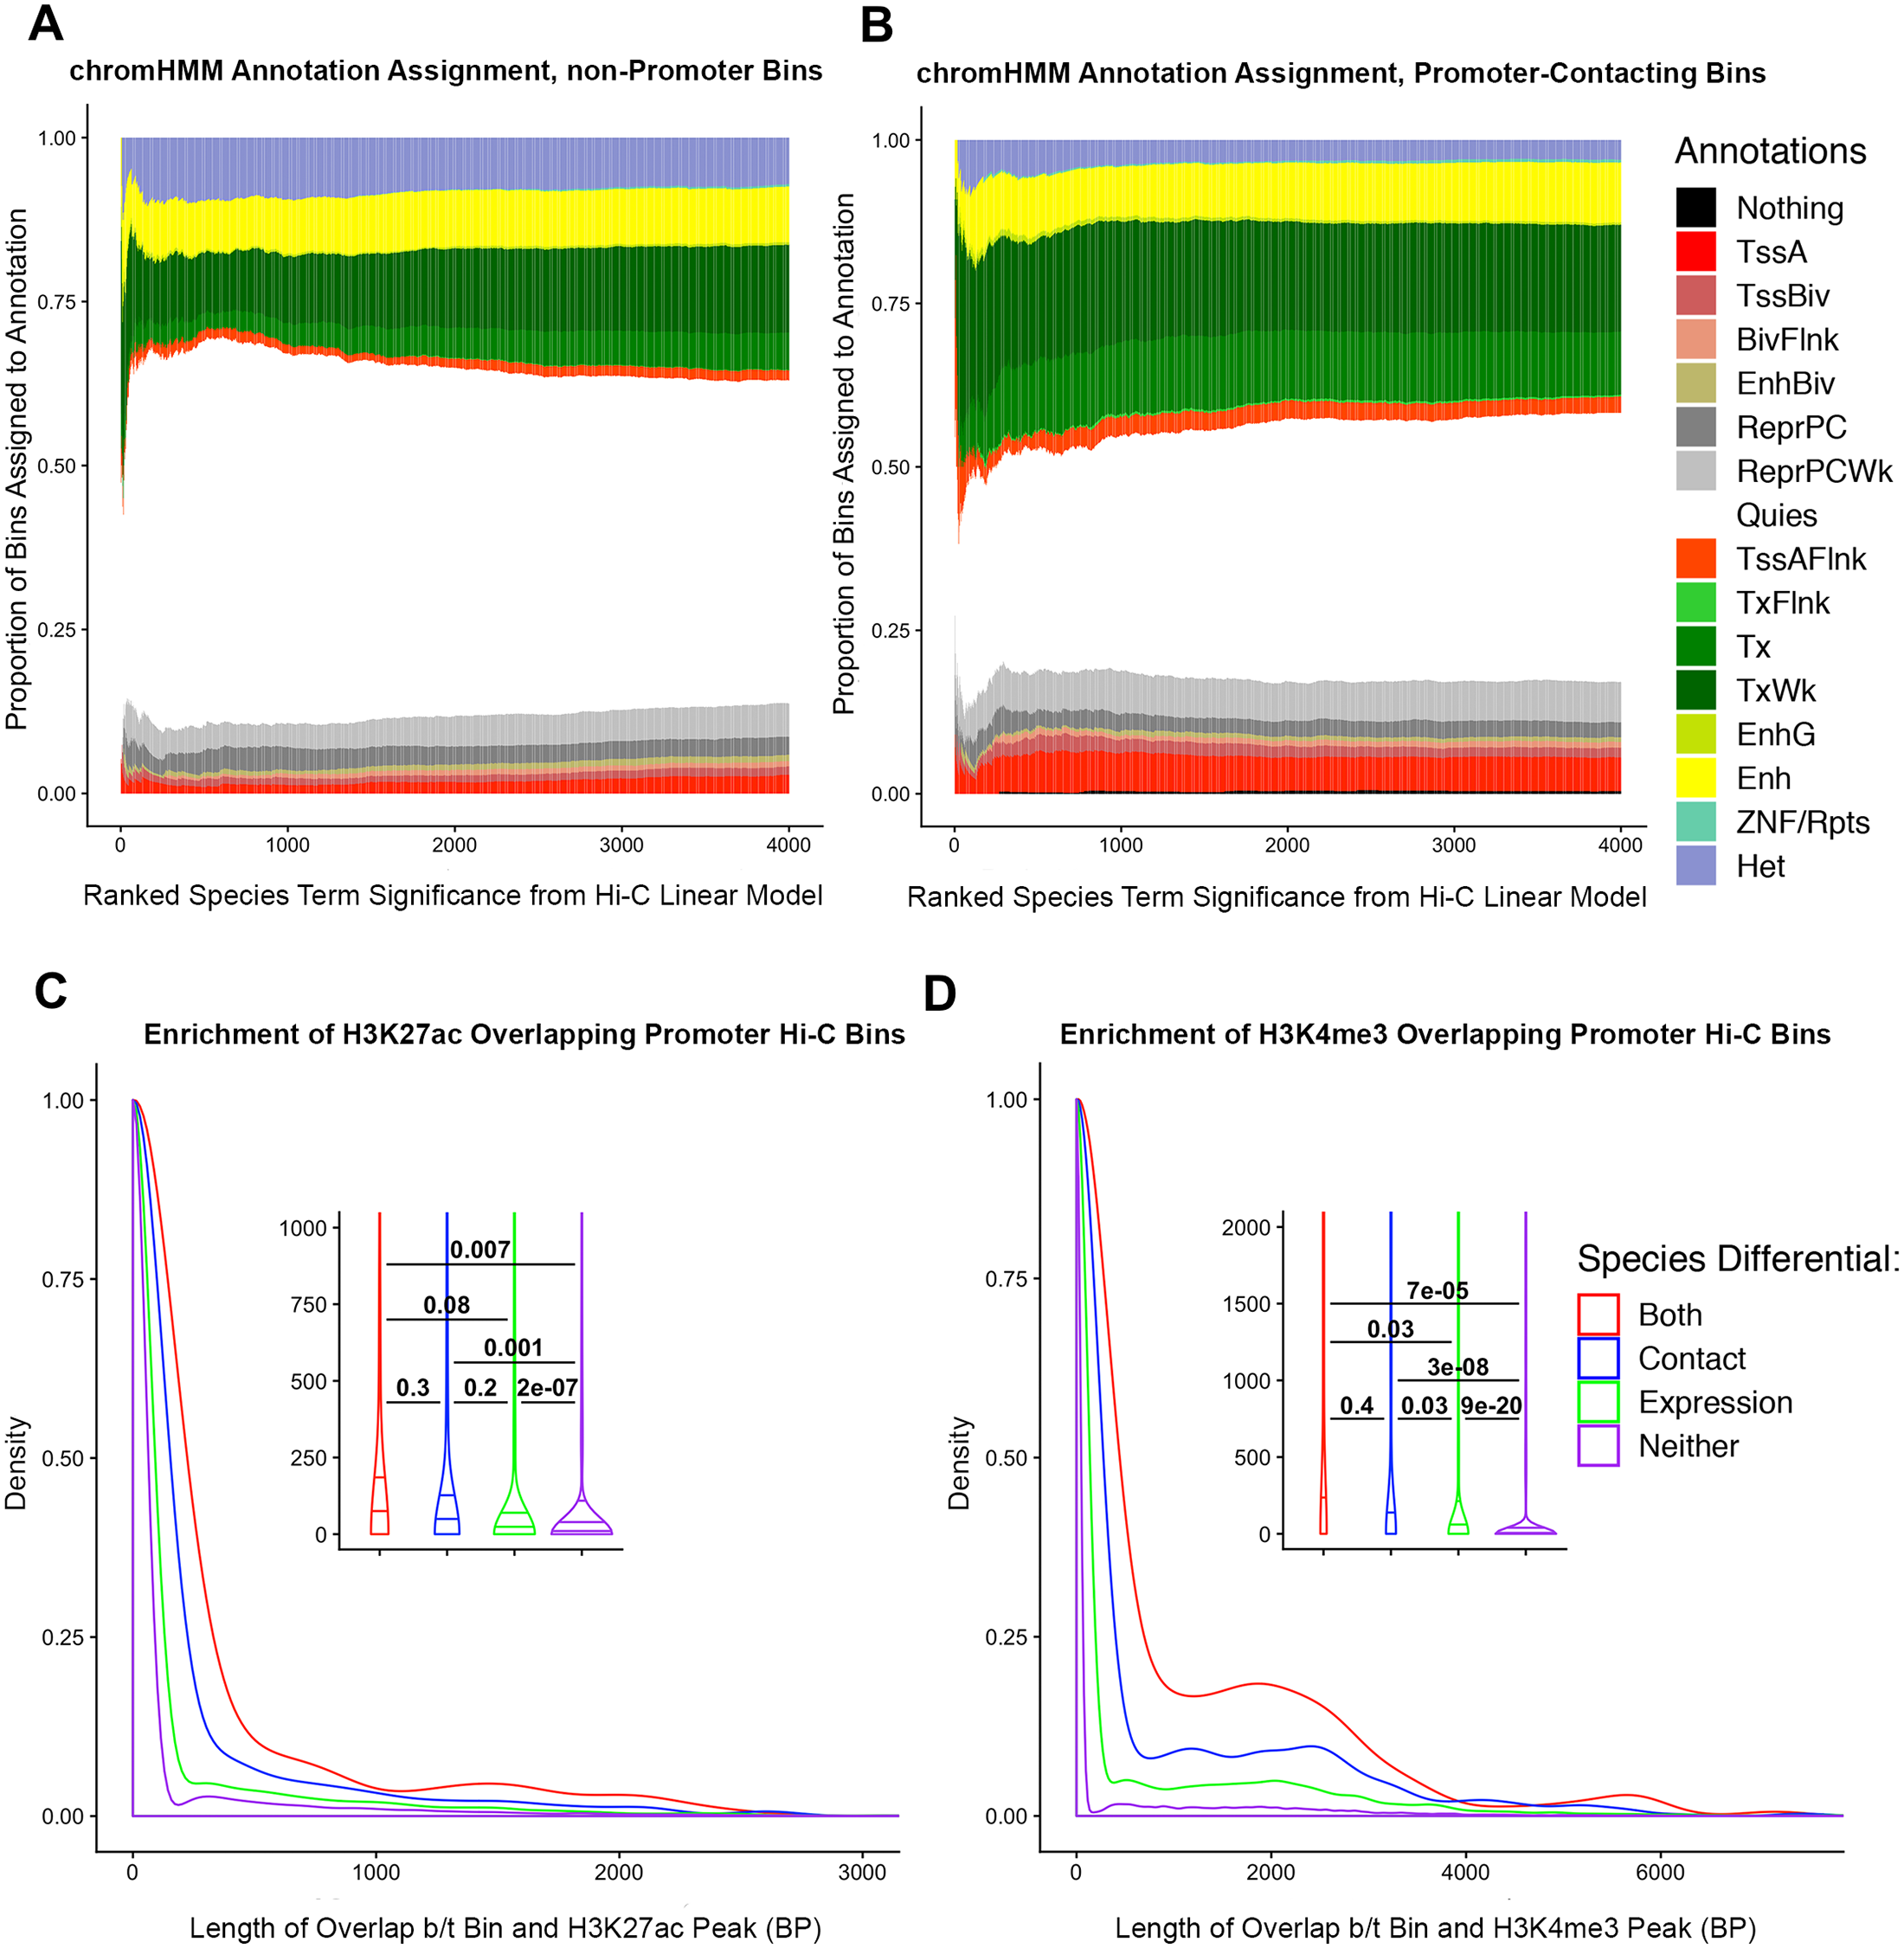
\includegraphics[width=4in]{img/fig7.PNG}
\caption[Overlap of epigenetic signatures and Hi-C contacts.]{\textbf{Overlap of epigenetic signatures and Hi-C contacts.} (A) Hi-C loci that do not make contact with promoters are ranked in order of decreasing DC FDR (x-axis). The y-axis shows cumulative proportion of chromHMM annotation assignments for all Hi-C loci at the given FDR or lower. (TssA-Active TSS, TSSBiv-Bivalent/Poised TSS, BivFlnk-Flanking Bivalent TSS/Enh, EnhBiv-Bivalent Enhancer, ReprPC-Repressed PolyComb, ReprPCWk-Weak Repressed PolyComb, Quies-Quiescent/Low, TssAFlnk-Flanking Active TSS, TxFlnk-Transcription at gene 5' and 3', Tx-Strong transcription, TxWk-Weak transcription, EnhG-Genic Enhancers, Enh-Enhancers, ZNF/Rpts-ZNF genes and repeats, Het-Heterochromatin). (B) Same as A, but only considering Hi-C loci making contact with promoter bins. Results of separating promoter-contacting bins between DE and non-DE genes can be seen in S19 Fig. (C) Density plot of the base pair overlap between different classes of Hi-C contact loci and H3K27ac. Histone mark data were obtained from ENCODE in experiments carried out in human iPSCs. We grouped contacts into 4 classes, indicated by color: those that show differential contact between species, those that show differential expression between species, those that show both, and those that show neither. We used pairwise t-tests to compare differences in the mean overlap among the four classes of Hi-C loci. (D) Same as C, but performed on H3K4me3 data obtained from ENCODE, collected in hESCs. Results with other histone marks can be seen in S18 Fig.}
\label{fig:ch02-fig7}
\end{figure}

We repeated the enrichment analysis of Hi-C regions using existing human iPSC histone mark data, including H3K27ac, H3K4me1, and H3K4me3, and h1-hESC histone mark data, including H3K27me3 and DNase I hypersensitivity sites (DHS \cite{consortium.2012a}). As expected, Hi-C regions in contact with a promoter showed greater overlap with DHS peaks than Hi-C regions that did not contact a promoter (t-test, P {\textless} 2.2 * 10\textsuperscript{-16}; S18A Fig). When we focused on contacts involving a promoter, we found that inter-species DCs that are also associated with DE genes showed the largest overlap with DHS peaks, followed by DE genes that were not associated with DC regions (P = 0.01). Regions that were not associated with either DC or DE showed the least amount of overlap with DHS (P = 0.0006; S18B Fig).

Remarkably, apart from the heterochromatic, repressive marker H3K27me3 (where the sign of the effect was the same, but the enrichment was not significant), Hi-C regions that are DC and are also associated with DE genes are more likely to overlap all other histone marks in our data set compared with Hi-C regions that are not DC and are not associated with a DE gene (all enrichment P {\textless} 0.03; Fig 7C and 7D, S18C and S18D Fig). In other words, inter-species DCs associated with DE genes are more likely to occur in genomic regions that are marked by histone modification, and are thus likely to have a regulatory function.

\pagebreak

\section{Discussion}\label{ch02-discussion}

In general, we observed lower-order, pairwise chromatin contacts in iPSCs to be conserved between humans and chimpanzees. We believe that this observation is intuitive, though we acknowledge that with only four individuals from each species, and given the challenges in identifying orthologous regions, we are likely to somewhat underestimate the degree of divergence in pairwise chromatin contacts.

In contrast to the conservation of lower order pairwise contacts, we did not find higher-order chromatin structures, such as TADs and TAD boundaries, to be generally conserved between human and chimpanzee iPSCs. Because this observation seems to contradict previous reports suggesting that TADs are strongly conserved across species \cite{Rao.2014, Dixon.2012}, we performed a large number of alternative analyses to demonstrate the robustness of our inference. Even in our most lenient analysis, we observed that only 78\% of domains are shared between humans and chimpanzees---a much lower conservation than observed for any other regulatory phenotypes between these two species (when similar sample sizes are considered; \cite{Pai.2011, Shulha.2012, Calarco.2007, Trizzino.2017, Prescott.2015}).

While all of the alternative analyses supported our inference, these analyses also demonstrated the known difficulty of robustly inferring TADs and TAD boundaries based on Hi-C data alone \cite{Ramirez.2018, Dali.2017}. Indeed, the algorithms used to infer TADs and TAD boundaries themselves are not very robust, as has been discussed previously \cite{Dali.2017, Forcato.2017}. Given our observations and the difficulty obtaining robust definitions of TADs and TAD boundaries, we carefully examined the previous evidence for high conservation of TADs between species.

The conclusion of our literature analysis is that the evidence for strong domain conservation is weak, and thus that our inference does not actually contradict previous data. A few of the studies typically cited as providing evidence for strong conservation of TADs across species did not actually perform a genome-wide assessment TADs, but inferred conservation based on a few examples \cite{Rudan.2015, Harmston.2017, Gomez-marin.2015}. Rudan et al. \cite{Rudan.2015}, for instance, reported functional conservation of TAD boundaries in liver cells from rhesus macaque, dog, rabbit, and mouse, but did not report the number or proportion of conserved regions they observed. Instead, they presented correlations of ~0.5 between contact frequencies across these species in subsets of contacts binned by the distance between mates, without further considering TADs or boundaries.

In contrast to studies that focused on specific examples, Dixon et al. \cite{Dixon.2012}, who originally described megabase-sized TADs at 40 kb resolution, reported that TAD boundaries were conserved in human and mouse embryonic stem cells. At a greater sequencing depth and finer resolution (1 kb), Rao et al. \cite{Rao.2014} observed TADs with a median size of 185 kb, and similar to Dixon et al., concluded that the domains were conserved in human and mouse B-lymphoblasts. However, the evidence for conservation in both studies is not strong. First, the actual conservation reported, though described as high, seems in fact to be modest: Dixon et al. reported that 54\% of human boundaries are shared with mouse (76\% if the comparison is reversed), and Rao et al. reported that 45\% of mouse domains are shared with human. Second, and more importantly, in both studies, conservation estimates were made unilaterally, by considering the proportion of TADs identified in the species for which they had less data that are also identified in the species for which they had more data. This approach results in an overestimate of sharing of domains because only the very strong TADs can be identified in the species with less data, and these are more likely to be shared across species. Indeed, if we perform a similar analysis using our own data (assessing sharing of the top 10\% of TADs identified in one species), we observe a much higher conservation (85\%). Conversely, if we use the data from Rao et al. to estimate reciprocal TAD sharing across species, conservation is even lower than originally reported, at $\sim$30\% instead of 45\%.

Thus, based on our analysis of the literature, we believe that the common notion that TADs are highly conserved in their placement across species is not well supported. Indeed, recent evidence from yeast \cite{Tjong.2012}, different Drosophila tissues \cite{Rowley.2017}, and plant species \cite{Dong.2017} suggests that TADs and TAD-like domains may not be particularly conserved, which raises questions about the stability of these higher-order structures and the significance of their role in the evolution of gene regulation across different lineages. However, the extent (or lack) of inter-species TAD conservation is difficult to falsify with existing data, partially because there is no standard method for identifying TADs, nor for comparing them across species \cite{Dali.2017, Forcato.2017}. The ability to reliably identify TADs also depends on the quality of the genome assemblies used, the approach for inferring synteny, sequencing depth and coverage, and various other parameters. We acknowledge that our estimates of inter-species differences in TADs may be somewhat inflated due to incomplete power to detect TAD structures in each genome. Unfortunately, the outputs of the available algorithms do not allow us to directly address this potential caveat in the same way we addressed incomplete power in the comparative analysis of lower-order interactions.

More generally, as many studies indicated \cite{Dali.2017, Yan.2017, Sauerwald.2018}, including ours, it is difficult to reconcile the visual examination of contact maps with TADs inferred based on algorithms. In our case (Fig 5 and S10 Fig), we found many examples where visual inspection naively suggests high conservation, but the algorithms do not indicate sharing of domains or boundaries. This is not surprising; a previous comprehensive analysis of numerous TAD algorithm inferences found very little concordance when compared to manual visual annotations of TADs \cite{Dali.2017}. Obviously, comparing all TAD inferences based on manual visual assessment is not feasible. Yet, the lack of stability of TAD algorithms means that it is possible that a better computational analysis will emerge and will indicate that domains or boundaries are indeed conserved. Currently, however, neither our own nor previously published data provides support for strong conservation of these structures.

\subsection{Contribution of variation in 3D genome structure to expression divergence}

We considered our Hi-C data along with gene expression data previously collected from the same cell lines \cite{Pavlovic.2018} and assessed the extent to which inter-species variation in 3D genome contacts could potentially explain gene expression divergence between species. Previous studies have observed that spatial co-expression of genes is associated with chromatin interaction profiles \cite{Babaei.2015, Dong.2010, Homouz.2013, Schoenfelder.2010, Duren.2017}. A number of studies have focused on differentially expressed genes following a treatment or perturbation and observed that such genes are often associated with corresponding differences in nearby chromatin contacts \cite{Dily.2014, Chen.2017}. Consistent with these reports, we found an enrichment of inter-species differences in pairwise chromatin contacts that involve promoters of differentially expressed genes between the species. Our observations are robust with respect to a range of data processing decisions and the statistical cutoffs we used. Under the common assumption that changes in chromatin contacts are more likely to explain differences in gene expression than vice versa, our results support the notion that species-specific 3D genomic contacts play an important role in the evolution of gene regulation.

Our observation that inter-species differences in pairwise genomic contacts are associated with regulatory evolution more than differences in large scale TAD boundaries is also consistent with previous reports. For example, Rao et al. \cite{Rao.2017} found that the degradation of cohesin, one of the proteins involved in maintaining TAD boundaries and large-scale loops, is associated with only modest effects on gene expression. In contrast, a number of other studies found strong correlations between differences in fine-scale genomic contacts and differences in the expression of nearby genes \cite{Rao.2014, Kagey.2010}.

Previous studies have identified a wide variety of regulatory phenotypes that contribute to inter-primate differences in gene expression levels \cite{Warner.2009, Loisel.2006, Pollard.2006, Pai.2011, Zhou.2014, Blekhman.2009, Cain.2011}; 3D genome conformation is only one of the putative upstream factors in the evolution of gene regulation. Our results argue for a model whereby inter-species differences in pairwise contact frequencies are among the main drivers of expression divergence between humans and chimpanzees. Given the low 10-kb resolution of our Hi-C data, it is likely that we have underestimated the contribution of inter-species variation in 3D genome structure to gene expression divergence between species. Future comparative Hi-C studies that sequence deeply enough to obtain higher, sub-kilobase resolutions, will allow researchers to resolve variation in contact frequency at even smaller scales, augmenting predictive power.

\subsection{Functional annotations}

Finally, we considered our data in the context of functional chromatin annotations available for the human genome. Previous studies have shown that 3D contact maps produced by Hi-C can be accurately recapitulated by epigenetic marks \cite{Pierro.2017, Zhu.2016}. Other reports have found enrichments for various chromatin accessibility and histone marks among interactions inferred from chromosome conformation capture data \cite{Roy.2015, Ron.2017}.

Our results corroborate and expand upon these findings. The differences we observed in chromHMM state assignments in our comparisons (namely, more active and less repressive states in promoter-involved contacts and contacts overlapping differentially expressed genes), provide additional support for the functional relevance of our inferences. We acknowledge that these differences could potentially be more pronounced with higher-resolution Hi-C data and with chromHMM inferences made from ChIP-seq experiments in the same cell lines. While our study design does not allow us to directly infer causality between chromatin interactions and gene expression, the functional enrichments we observed for different epigenetic marks suggest that 3D genome conformation may be one of the upstream elements in the chain of events driving the evolution of gene expression. Although this notion is intuitive to us and is consistent with our data, it is still possible that differences in epigenetic marks are the true drivers of divergence in gene expression levels and/or chromatin contacts between humans and chimpanzees.

Future studies integrating similar data types could explore these possibilities by examining epigenetic marks across species (only human data were available to us), which would enable researchers to polarize the regulatory differences in orthologous sequences between humans and chimpanzees. This would also allow for a sharper definition of the functional classes of inter-species differences in lower-order chromatin contacts.

\section{Materials and methods}

\subsection{Ethics statement}

We collected human fibroblasts with written informed consent obtained from all human participants under University of Chicago IRB protocol 11---0524. We obtained fibroblasts from chimpanzees from the Yerkes Primate Research Center of Emory University under protocol 006---12, in full compliance with IACUC protocols \cite{Romero.2015}. All experimental methods are in accordance with the Helsinki Declaration.

\subsection{Induced pluripotent stem cells (iPSCs)}

As described previously, the Gilad lab has derived panels of both human and chimpanzee iPSCs via episomal reprogramming \cite{Romero.2015}. To ensure their quality, we validated iPSCs from both species as pluripotent at high passages ({\textgreater}10). Quality control checks included an embryoid body assay confirming their ability to differentiate into all three germ layers, qPCR of endogenous transcription factors associated with pluripotency, PCR to confirm the absence of exogenous pluripotency genes (both from residual episomal plasmid or genomic integration), and PluriTest \cite{Muller.2011}, a bioinformatics classifier that assesses pluripotency based on gene expression data \cite{Romero.2015}. In the current study, we grew all cell lines in the same incubator in two passage-matched batches, which were also balanced across species and sex, in order to avoid batch effects in our data.

\subsection{In-situ Hi-C library preparation and sequencing}
We performed \textit{in situ} Hi-C with the restriction enzyme MboI, as previously described \cite{Rao.2014} on the iPSCs from both species. We grew cells in feeder-free conditions \cite{Nakagawa.2014} to approximately 80\% confluence before adding formaldehyde to crosslink the proteins mediating DNA-DNA contacts. We flash-froze pellets of 5 million cells each before beginning the in situ Hi-C protocol \cite{Rao.2014}. We used MboI to cut the DNA at each of its 4-bp recognition sites (GATC) throughout the genome. Ligation of proximal fragments with T4 DNA ligase yielded chimeric DNA molecules representing two distinct loci. Libraries were created in two balanced batches identical to the cell growth batches and sequenced (100bp paired-end) on an Illumina Hi-Seq 4000 at the University of Chicago Genomics Core Facility. To avoid batch effects resulting from differences in flow cells, libraries were sequenced across three lanes, each on separate flow cells balanced for species.

\subsection{Hi-C read mapping, filtering, and normalization}

We preprocessed, mapped, and filtered the resulting FastQ sequence files using HiCUP version 0.5.9 \cite{Wingett.2015}. We also used HiCUP to truncate the reads at ligation junctions. Thereafter, we used bowtie2 version 2.2.9 \cite{Langmead.2012} to independently map the two mates of paired-end sequences to either the hg38 or panTro5 genomes, and removed reads with low quality scores (MAPQ {\textless} 30). We carried out further HiCUP filtering as previously described based on an \textit{in silico} genome digest in order to remove experimental artifacts \cite{Wingett.2015}. We then used HOMER version 4.9.1, a foundational statistical analysis suite for Hi-C data \cite{Heinz.2010}, to tile the genome into a matrix of 10 kb bins and assign reads to their corresponding intersecting bins. We subsequently used HOMER to normalize Hi-C contact bins as previously described \cite{Heinz.2010}, accounting for known technical biases in Hi-C data. Finally, we called statistically significant interactions independently in each individual using HOMER, based on a null expectation of read counts falling into bins in a cumulative binomial distribution \cite{Heinz.2010}. We retained interactions with an unadjusted P value ${\leq}$ 0.01, the default recommendation by HOMER. As other studies have noted \cite{Durand.2016}, a traditional multiple testing correction paradigm is overly conservative for Hi-C data due to the high number of tests, and because the spatial nature of the data means that individual tests are highly correlated (and thus not independent).

\subsection{Creation of a union list of orthologous Hi-C contacts across species}

In order to ensure that the contact frequencies we compared across species were from representative orthologous sequences in humans and chimpanzees, we used liftOver with a reciprocal best hits method \cite{Ward.2014, Kent.2002} to transfer interaction bin coordinates across both genomes. For each called contact, we used liftOver to independently map the coordinates of the two anchor bins in the other species' genome, obtaining coordinates in both genomes for all contacts. We then rounded the coordinates to the nearest 10 kb bin, in order to align properly with a Hi-C bin. We required both anchor bins to have orthologous bins in the other species in order to retain a contact for comparison; statistics on the number of called contacts and the number retained after our liftOver procedure are available in S9 Table. In order to assess the extent of contacts lost due to lack of orthology, we also compared the retention of genome-wide 10 kb bins in both genomes with the retention of unique 10 kb bins found within each of our individuals. We found that our Hi-C bins tended to have a higher rate of orthologous mappability across species (S9 Table). For all contacts in this union list, we then extracted the HOMER-normalized interaction frequencies from each individual's 10 kb Hi-C matrix. Including interactions discovered in fewer than 4 individuals increased the variance in our data (S7 Fig). Therefore, we retained only the Hi-C contacts that were independently discovered by HOMER in at least 4 individuals, for a total of 347,206 interactions. As we describe in the next section, we also later filtered out contacts where the distance between bins showed a difference of {\textgreater} 20 kb across species, retaining 292,070 interactions.

\subsection{Linear modeling of Hi-C interaction frequencies}

In an effort to quantify inter-species differences in the Hi-C interaction frequency values, we used the following linear model:

\begin{equation} \label{eq:limma}
Y_{ij} = \beta_{0} + \beta_{sp}s_{i} + \beta_{sx}x_{j} + \beta_{btc}b_{i} + \epsilon_{ij}
\end{equation}

$Y_{ij}$ represents the observed Hi-C interaction frequency of a contact from individual j in species i. $\beta_{0}$ is the intercept. $\beta_{sp}$, $\beta_{sx}$, and $\beta_{btc}$ are effect sizes for species, sex, and batch, respectively, with their corresponding variables $s_{i}$, $x_{j}$, and $b_{i}$, and an error term $\epsilon_{ij}$. We used the R/Bioconductor package limma \cite{Smyth.2004, Law.2014} to test for inter-species differences in Hi-C interaction frequency. We applied Benjamini-Hochberg multiple testing correction and found 13,572 interaction pairs where the species term is significant at a 5\% false discovery rate (FDR).

Initial visualization of the linear modeling results for the species term revealed a stark asymmetry (S9A Fig) suggesting that on a global level, the contacts identified as significant in chimpanzees were much stronger than those identified in humans. This was surprising to us; we reasoned that this asymmetry could be due to a technical factor. For example, liftOver conversion of genome coordinates between species to identify orthologous bins can create differences in both the Hi-C locus size and in the genomic distance between mates of a contact pair (mate-pair distance). We investigated the impact of these two factors on the proportion of contacts classified as differential across species in our data. We discovered that while changes in Hi-C locus size had little effect on the proportion of interspecies DCs, differences in mate-pair distances {\textgreater} 20 kb across species created a noticeable inflation in this proportion at an FDR of 5\% (S9B Fig). We believe this makes intuitive sense, as bins that are farther apart will have fewer read counts due to the proximity-based ligation in Hi-C. Thus, a mate-pair distance difference across the genomes could induce what appears to be a differential contact, because the contact inherently has more read support in the species where the mates are closer. However, we note that it is impossible to ascertain the relative biological and/or technical relevance of the differences seen in these contacts. We thus took a conservative approach to minimize false positives and removed contacts with a {\textgreater}20 kb mate-pair distance difference between species from our downstream analyses (S9 Fig), accepting that the number of inter-species differences we observe may be underestimated.

\subsection{Identification of orthologous topologically associating domains (TADs) and boundaries}

We chose to perform TAD analyses on both individual-level data and on representative species consensus data. For our analysis comparing TAD boundaries on species consensus Hi-C maps, we combined all the preprocessed Juicer files from all our individuals within a species and used the \textit{juicer\_mega.sh} script \cite{Durand.2016} to create higher density contact maps for each species. We then ran the Arrowhead algorithm across resolutions to infer TADs, and then we extended the edges of TADs 7.5 kb in each direction to create 15 kb boundaries (accounting for imprecision in boundary inference). We used a reciprocal best hits liftOver strategy \cite{Ward.2014, Kent.2002} to obtain orthologously mappable TADs and boundaries. To confirm high synteny of large-scale linear genomic intervals between the species, we employed this same orthology analysis on genome-wide tilings of the hg38 and panTro5 genome assemblies, with varying window sizes created with bedtools \cite{Quinlan.2010} \textit{makewindows} (S11 Fig). In the case of TADs, we then assessed number of domains found in one species that were also found in the other species (conserved domains) with reciprocal bedtools \cite{Quinlan.2010} \textit{intersect {\textendash}c {\textendash}f 0.9 -r} calls. These parameters will only define a domain as overlapping if there is a domain in the other species such that each domain shares 90\% of their interval with the other. We used the larger of the two estimates of shared TADs across the species as the conserved domain count (to be conservative), and divided this by the sum of the conserved and species-specific domains identified in order to assess conservation. As an alternative analysis, we also employed the method previously described by Rao et al. \cite{Rao.2014}; namely, we called a TAD conserved in one species if it and a TAD from the other species displayed a Euclidean distance less than the smaller of 50 kb or half the given TAD's size. We analyzed boundary conservation using bedtools \textit{intersect {\textendash}c}, considering any overlap as indication of conservation (i.e. even a single base pair overlap of boundaries meant a boundary was classified as conserved).

To examine individual-level data and to ensure robustness of our results, we separately used both Arrowhead \cite{Durand.2016} and TopDom \cite{Shin.2016} (with \textit{window = 20}) across resolutions to call TADs independently in each individual sample. Though we performed essentially the same analyses on both outputs, it should be noted that Arrowhead provides nested TADs only, from which we inferred boundaries as described above, whereas TopDom provides separate domain and boundary inferences. We used a reciprocal best hits liftOver method \cite{Ward.2014, Kent.2002} to obtain a set of orthologous domains and boundaries. We assessed interspecies conservation by performing left outer joins (bedtools \textit{intersect {\textendash}loj}) of each individual's domains against all the others, once again requiring 90\% reciprocal overlap. We then took the average species-specific and shared domain counts across these individual comparisons to produce a single estimate of conservation (S12 and S14 Figs). The individuals' pairwise percentages of shared domains were used in hierarchical clustering analysis (Fig 4C, S12 and S14 Figs). We also once again checked the robustness of our results using the conservation calling method from Rao et al. \cite{Rao.2014} described above. In the case of boundaries, we reasoned that, given the nested nature of the TADs, as well as variance between individuals in their exact placement, it would make sense to merge the boundaries (using bedtools \textit{merge}) in order to obtain a list of unique boundary elements. We added a column of individual identifiers to each set of boundaries and then merged all together, thereafter assessing conservation by examining what percentage of boundaries were independently found in both species out of the total set of unique boundaries. We also applied hierarchical clustering analysis to individual pairwise percentages of shared boundaries in this union merged file (Fig 4D, S12 and S14 Figs). Further descriptions of these analyses can be found on our GitHub repository (/data/TADs folder), and 10 kb individual Arrowhead inferences are available in S17{\textendash}S24 Tables.

\subsection{Differential expression analysis}

Previously, the Gilad lab generated RNA-seq expression data on the same iPSC lines from this study (GEO accession GSE110471 \cite{Pavlovic.2018}). We computed reads per kilobase per million mapped reads (RPKM) for every gene, as the orthologous genes are not constrained to be the same length across species. We retained 11,074 genes that had at least half of the individuals (2 observations) in each species with log\textsubscript{2}RPKM ${\geq}$ 0.4. We then used the limma-voom pipeline with precision weights \cite{Smyth.2004, Law.2014} to test for differential expression across species, using a linear model including a species effect and a sex effect. Using this approach, we found 2,086 differentially expressed genes (at 5\% FDR).

\subsection{Broad integration of Hi-C and gene expression data}

We obtained the overlap between our gene expression data and our Hi-C data by applying bedtools \textit{overlap} \cite{Quinlan.2010} to the Hi-C loci and the first exon of each gene. Using a curated file of orthologous gene coordinates between humans and chimpanzees \cite{Pavlovic.2018}, we extracted a one-base-pair interval at the beginning of each first exon to use as a proxy for transcription start sites (TSSs).

As described in the main text, the difference in dimensionality between the two datasets presented a challenge. While every gene has only one expression value per individual, a given Hi-C locus can and frequently does make contact with many other loci. When a given gene overlapped a Hi-C locus making multiple contacts, we chose the contact with the smallest species term FDR (i.e. the most species-specific contact) in our DC analysis to represent the interaction frequency for that gene. Accordingly, we interpreted the FDR-adjusted P value for the chosen contact as the gene's differential contact significance. To examine correlations between normalized Hi-C contact frequency and log\textsubscript{2}RPKM gene expression, we considered the correlation between gene expression values across all 8 individuals with the corresponding interaction frequency values across the same 8 individuals.

\subsection{Enrichment of differential expression in differential contacts}

We examined the enrichment of differential expression in genes with differential contact (Fig 6A and S20C Fig) across a continuous range of DC FDRs and a discrete range of DE FDRs (1\%, 2.5\%, 5\%, 7.5\%, and 10\%). We used Pearson's chi-squared test to quantify significance of the enrichment at each FDR (Fig 6B and S20D Fig). We also examined the reciprocal enrichment; that is, DC enrichment amongst DE genes (S20A and S20B Fig).

\subsection{Assessing the quantitative contribution of Hi-C contact frequencies to gene expression levels}

We assessed the hypothesis that expression divergence may be mediated by contact frequency using linear models \cite{Baron.1986}. The intuition behind this approach is that the effect of species (X) on expression (Y) can be partitioned into its indirect effect on expression mediated through contact frequency (M) and its direct effect on expression. Therefore, a significant indirect effect would suggest that expression divergence is causally mediated by contact frequency. To test our mediation hypothesis, we computed the indirect effect of species on expression (X $\rightarrow$ M $\rightarrow$ Y: causal effect of X on Y through M) by taking the product of the effect of species on contact frequency ($\alpha$: X $\rightarrow$ M) and the effect of contact frequency on expression after controlling for species ($\beta$: M $\rightarrow$ Y). The indirect effect ($\alpha$*$\beta$) is conceptually equivalent to the difference between the effect of species on expression and the effect of species on expression after controlling for contact frequency, but is more mathematically tractable and commonly used in mediation analyses \cite{Sobel.1986, Sobel.1982, MacKinnon.2002}. We obtained $\alpha$ as the species effect size in a simple linear model attempting to predict Hi-C interaction frequency based solely on a species term. We estimated $\beta$ as the contact frequency effect size in a linear model predicting expression based on both species and contact frequency per gene. To determine statistical significance of the indirect effect, we applied the Monte Carlo test of significance to construct the 95\% confidence interval. The primary benefits of the Monte Carlo method are that it requires no distributional assumptions of the data and is robust against type I error in small samples \cite{MacKinnon.2004, Preacher.2012, Preacher.2004}. Thus, we choose the Monte Carlo test over Sobel test, the conventional approach to significance testing of mediation, which relies on the data following normal distribution \cite{Sobel.1986, Sobel.1982}.

\subsection{Integration with epigenetic annotations}

We obtained chromHMM 15-state model peak calls in human iPSC cells from ENCODE \cite{consortium.2012a} (S15 Table). We subsequently found the overlap between the human coordinates of our orthologous Hi-C contact loci and the chromHMM peak calls and quantified the extent of base pair overlap between each locus and all overlapping chromHMM peaks. We assigned each individual locus a single chromHMM annotation based on the peak with the highest base pair overlap with that locus. However, the distribution of overlaps of different chromHMM annotation peaks with our Hi-C bins were quite variable in size. To account for this, we normalized each annotation's overlap length in each locus by multiplying it by the reciprocal of its mean base pair overlap across all our bins (S17 Fig). After removing duplicate Hi-C loci, we then assigned individual loci to chromHMM annotations based on these normalized base pair overlaps. We started with a small set of the top ten most differentially contacting loci (i.e. the ten lowest FDR loci from our Hi-C linear modeling), and tabulated proportions of which annotations were represented amongst them. We then iteratively added the next-lowest FDR contact (i.e. two Hi-C loci at a time) to this tabulation, re-calculating proportions on the new set of contacts. We ran this same cumulative proportions analysis separately on contacts not overlapping promoters, contacts overlapping promoters, contacts overlapping promoters of DE genes, and contacts overlapping promoters of genes that were not DE (Fig 7A and 7B, S19 Fig).

We also obtained data on H3K4me1, H3K4me3, and H3K27ac collected in human iPS-18A cells, and data on H3K27me3 and DNase hypersensitivity sites collected in H1-hESCs, all from ENCODE \cite{consortium.2012a} (S15 Table). We used bedtools \textit{intersect} \cite{Quinlan.2010} to find the base pair overlap between each of these different marks and our Hi-C contact loci. We then removed duplicate Hi-C loci from the dataset and used a pairwise t-test to identify significant differences in the overlapping distributions for different sets of Hi-C classes (based on differential contact and differential expression, Fig 7C and 7D).

\section{Acknowledgments}

We thank the members of the Gilad, Nobrega, and Stephens labs for helpful discussions, particularly Matthew Stephens, Bryan J. Pavlovic, D\'ebora R. Sobreira, Abhishek Sarkar, and Lindsey E. Montefiori. We thank Natalia Gonzales for help editing the paper.

\subsection{Author contributions}

IEE and YG conceived of the study and designed the experiments. IEE performed the experiments. IEE analyzed the results (with input from CJH, KL, and LEB). YG supervised the project. IEE and YG wrote the paper. All authors read and approved the final manuscript.

\pagebreak
\clearpage

\section{Supplementary Figures}\label{ch02-supplementary-figures}

\begin{figure}[!htb]
\centering
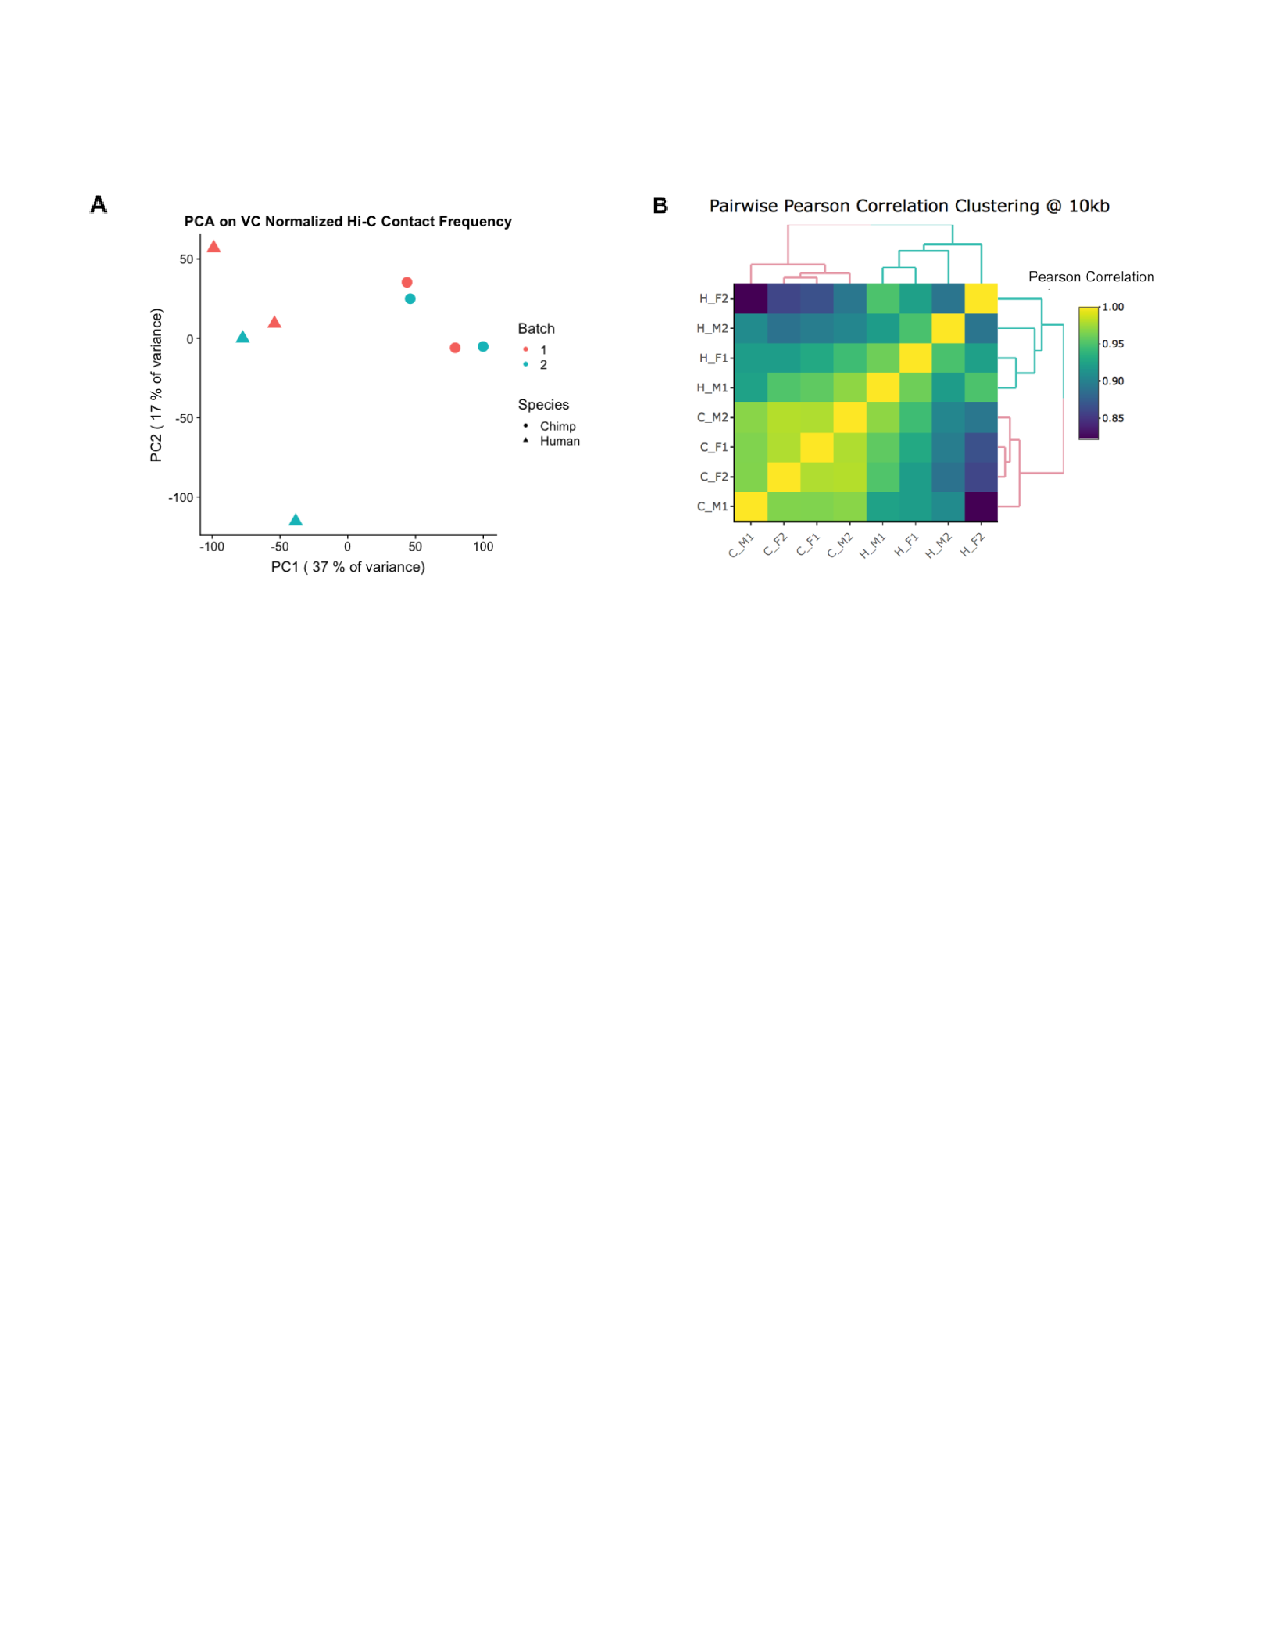
\includegraphics[width=6in]{img/figS1.pdf}
\caption[Regulatory landscapes cluster by species, Juicer.]{\textbf{S1. Regulatory landscapes cluster by species, Juicer.} (A) Principal components analysis (PCA) of Juicer vanilla coverage (VC)-normalized interaction frequencies for the union of all contacts in humans (triangles) and chimpanzees (circles). PC1 is highly correlated with species (r = 0.89; P = 0.0004). (B) Unsupervised hierarchical clustering of the pairwise correlations (Pearson's $r^2$) of Juicer VC-normalized interaction frequencies at 10 kb resolution. The first letter in the labels demarcates the species (H for human and C for chimpanzee), and the following symbols indicate sex (male, M or female, F) and batch (1 or 2).}
\label{fig:ch02-figS1}
\end{figure}

\begin{figure}[!htb]
\centering
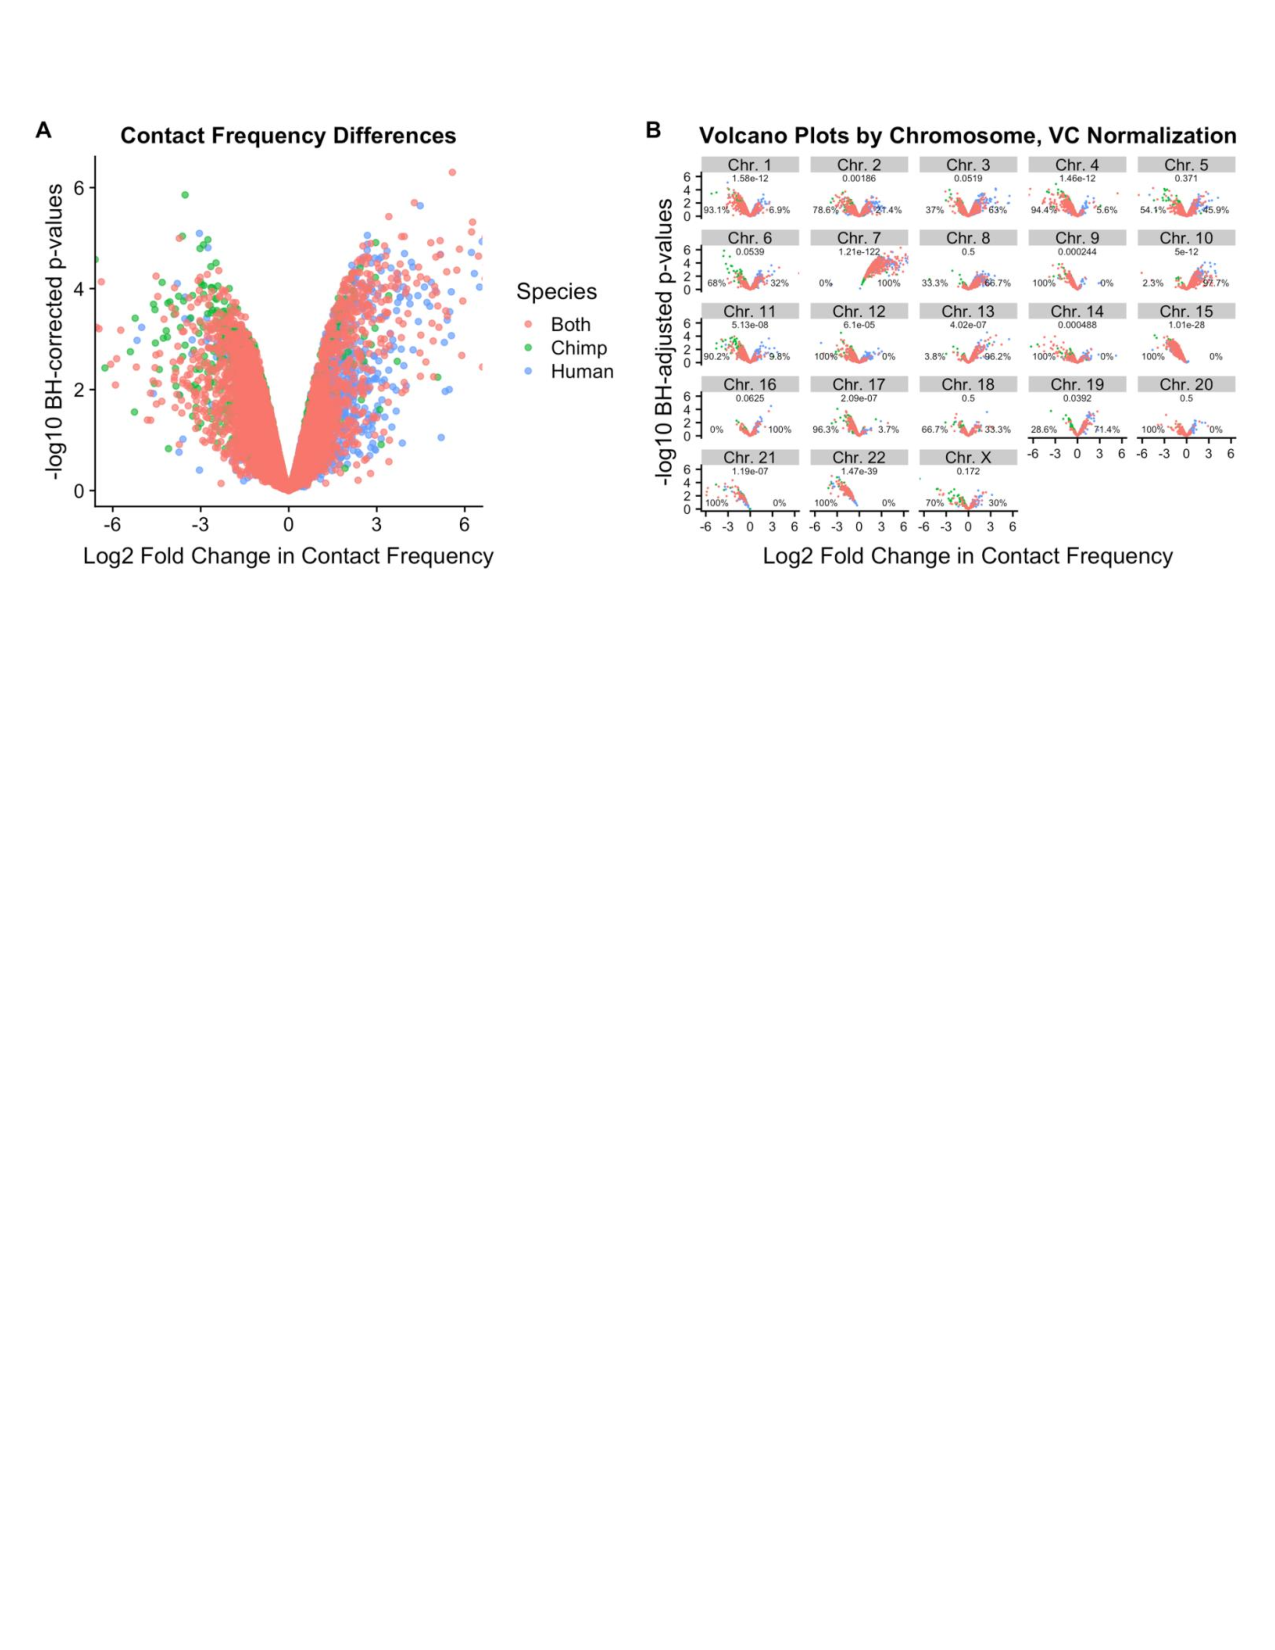
\includegraphics[width=6in]{img/figS2.pdf}
\caption[Linear modeling reveals large-scale chromosomal differences in contact frequency, Juicer.]{\textbf{S2. Linear modeling reveals large-scale chromosomal differences in contact frequency, Juicer.} (A) Volcano plot of log\textsubscript{2} fold change in contact frequency between humans and chimpanzees (x-axis) against Benjamini-Hochberg FDR (y-axis), after filtering non-orthologous regions. Data are colored by the species in which the contact was originally identified as significant. (B) Per-chromosome volcano plot using the same legend as in A. P-values provided for a binomial test of the null that inter-species differences in contact frequencies are evenly distributed. The percentage of contacts with significant higher frequency in each species is noted. Of note is that many of the same chromosomal asymmetries in contact strength observed here are in the same chromosomes as those observed in the HOMER-normalized data (Fig 2).}
\label{fig:ch02-figS2}
\end{figure}

\begin{figure}[!htb]
\centering
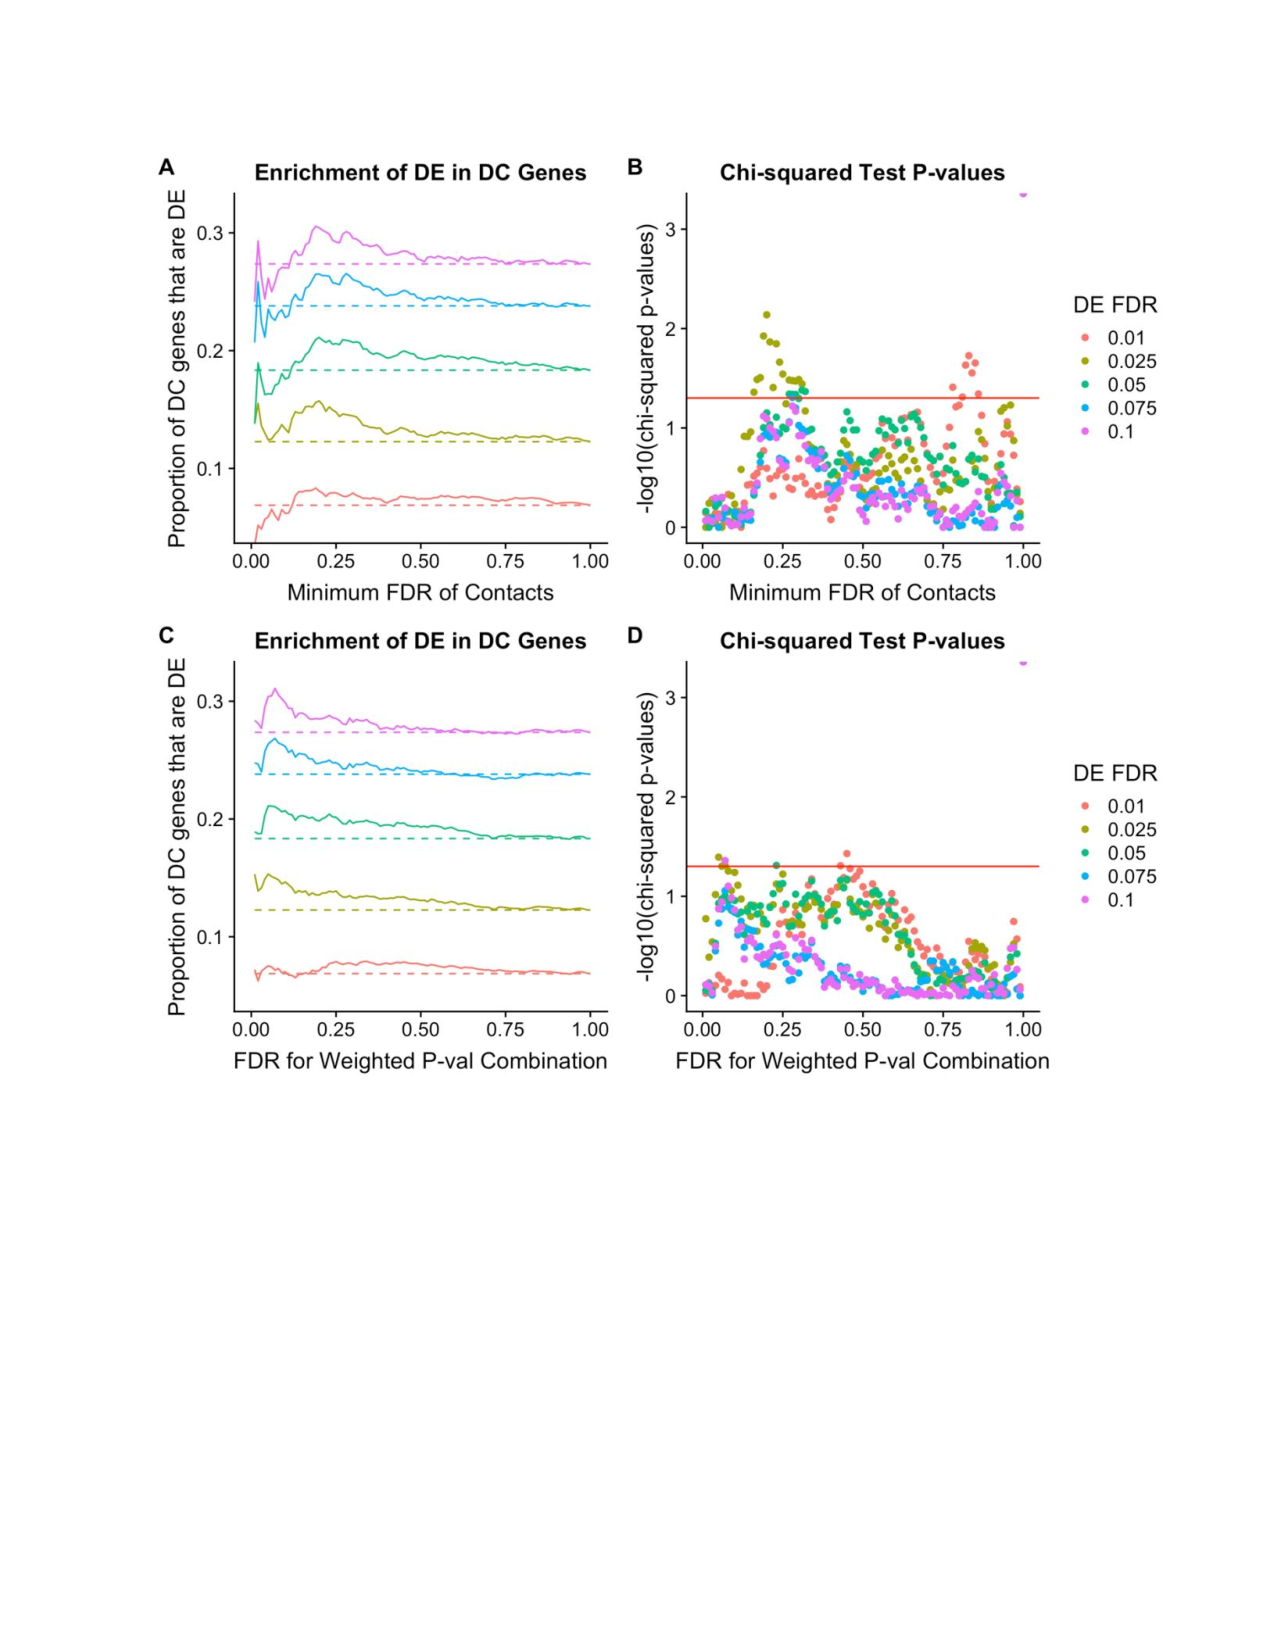
\includegraphics[width=6in]{img/figS3.pdf}
\caption[Differentially expressed genes show enrichment for differential Hi-C contacts, Juicer.]{\textbf{S3. Differentially expressed genes show enrichment for differential Hi-C contacts, Juicer.} (A) Enrichment of inter-species differentially expressed (DE) genes with corresponding differences in Hi-C contact frequencies (DC) between the species. The proportion of DC genes that are significantly DE (y-axis) is shown across a range of DC FDRs (x-axis). Colors indicate different DE FDR thresholds, and dashed lines indicate the proportion of DE genes expected by chance alone. (B) P values of Chi-squared tests of the null that there is no difference in proportion of DE genes among DC genes (y-axis), shown for a range of DC FDRs (x-axis). In both panels, DC regions were chosen to have the minimum FDR supporting inter-species difference in contact frequency. (C) Same as A, but this time, a weighted p-value combination technique \cite{Whitlock.2005} was used to integrate each Hi-C bin's DC FDR across all of its contacts. (D) Same as B, but for the weighted p-value combination instead of the minimum FDR contact.}
\label{fig:ch02-figS3}
\end{figure}

\begin{figure}[!htb]
\centering
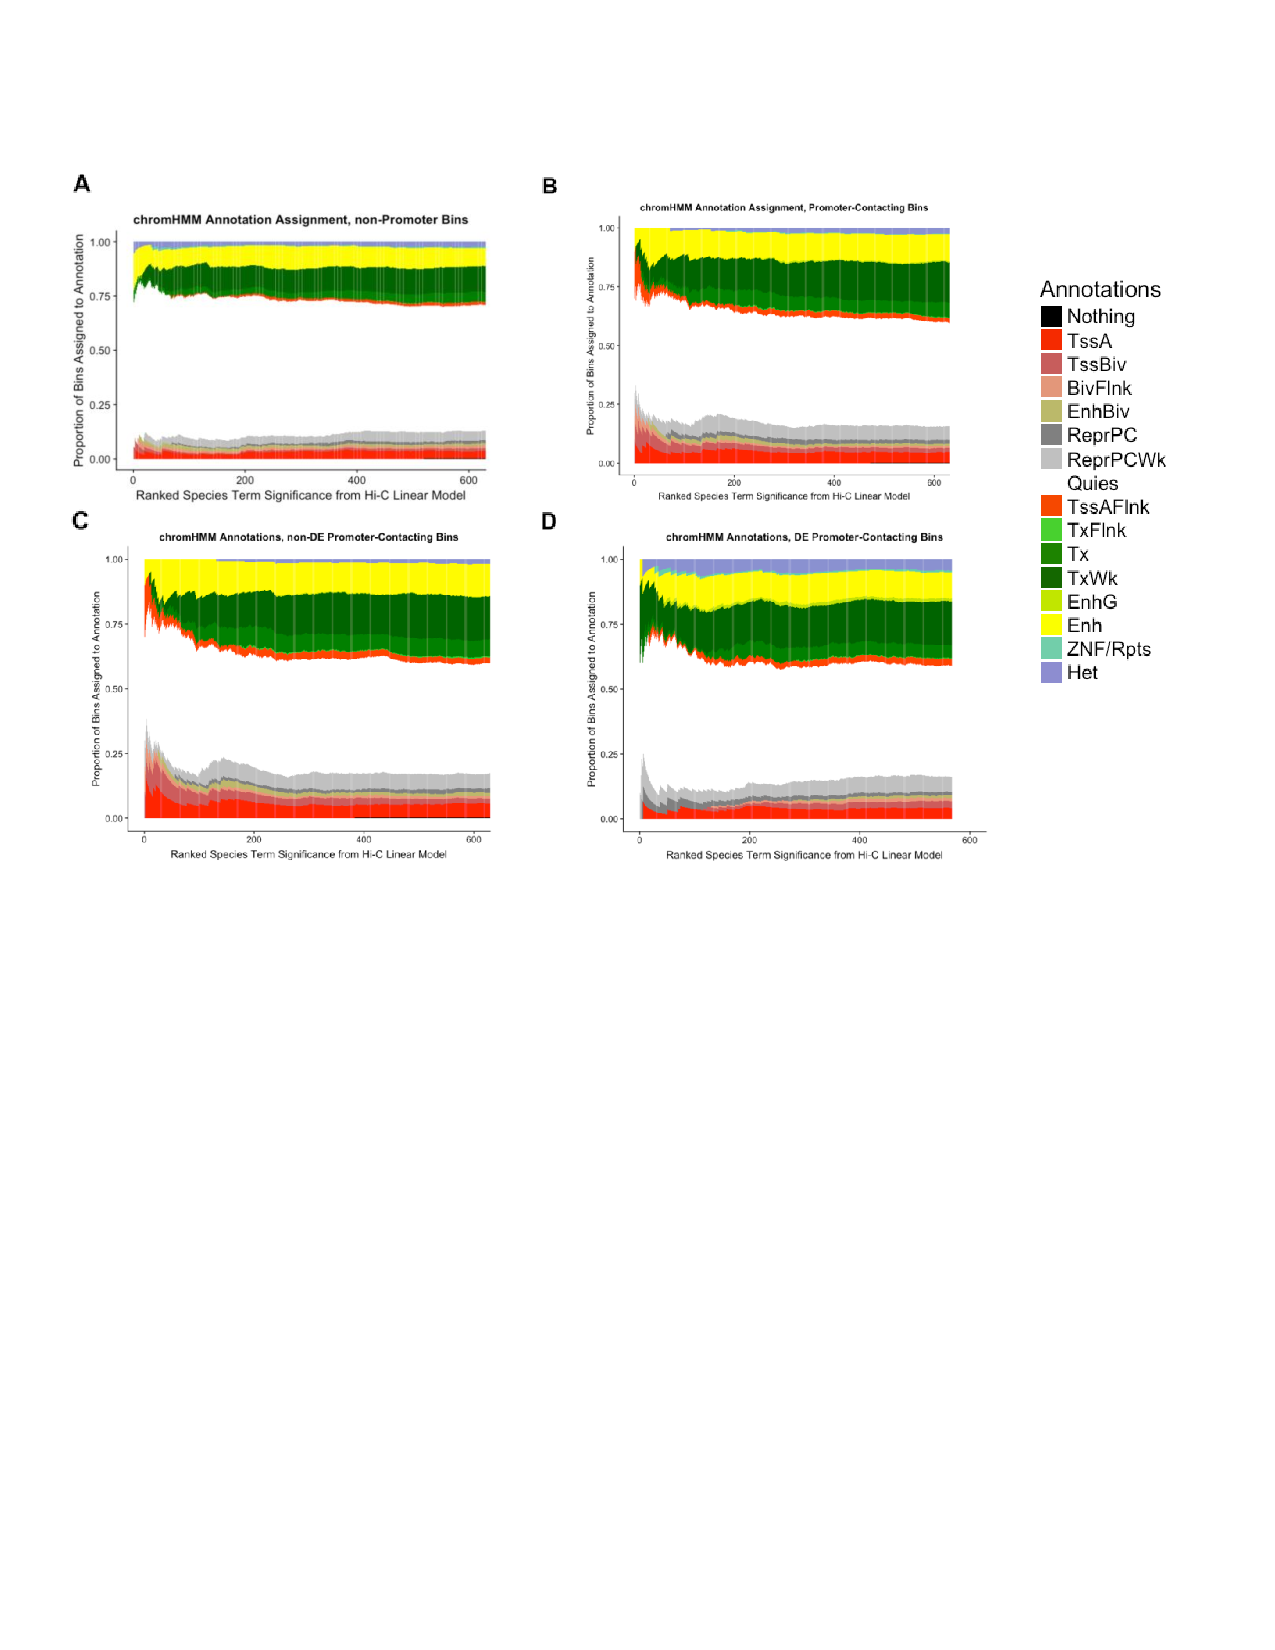
\includegraphics[width=6in]{img/figS4.pdf}
\caption[Dynamics of chromHMM state among significant Hi-C contacts, Juicer.]{\textbf{S4. Dynamics of chromHMM state among significant Hi-C contacts, Juicer.} (A) Hi-C loci that do not make contact with promoters are ranked in order of decreasing DC FDR (x-axis). The y-axis shows cumulative proportion of chromHMM annotation assignments for all Hi-C loci at the given FDR or lower. (TssA-Active TSS, TSSBiv-Bivalent/Poised TSS, BivFlnk-Flanking Bivalent TSS/Enh, EnhBiv-Bivalent Enhancer, ReprPC-Repressed PolyComb, ReprPCWk-Weak Repressed PolyComb, Quies-Quiescent/Low, TssAFlnk-Flanking Active TSS, TxFlnk-Transcription at gene 5' and 3', Tx-Strong transcription, TxWk-Weak transcription, EnhG-Genic Enhancers, Enh-Enhancers, ZNF/Rpts-ZNF genes and repeats, Het-Heterochromatin). (B) Same as A, but only considering Hi-C loci making contact with promoter bins. (C) Same as B, but only considering Hi-C loci making contact with promoters of genes that are not differentially expressed (DE). (D) Same as C, but only considering Hi-C loci making contact with promoters of genes that are differentially expressed (DE).}
\label{fig:ch02-figS4}
\end{figure}

\begin{figure}[!htb]
\centering
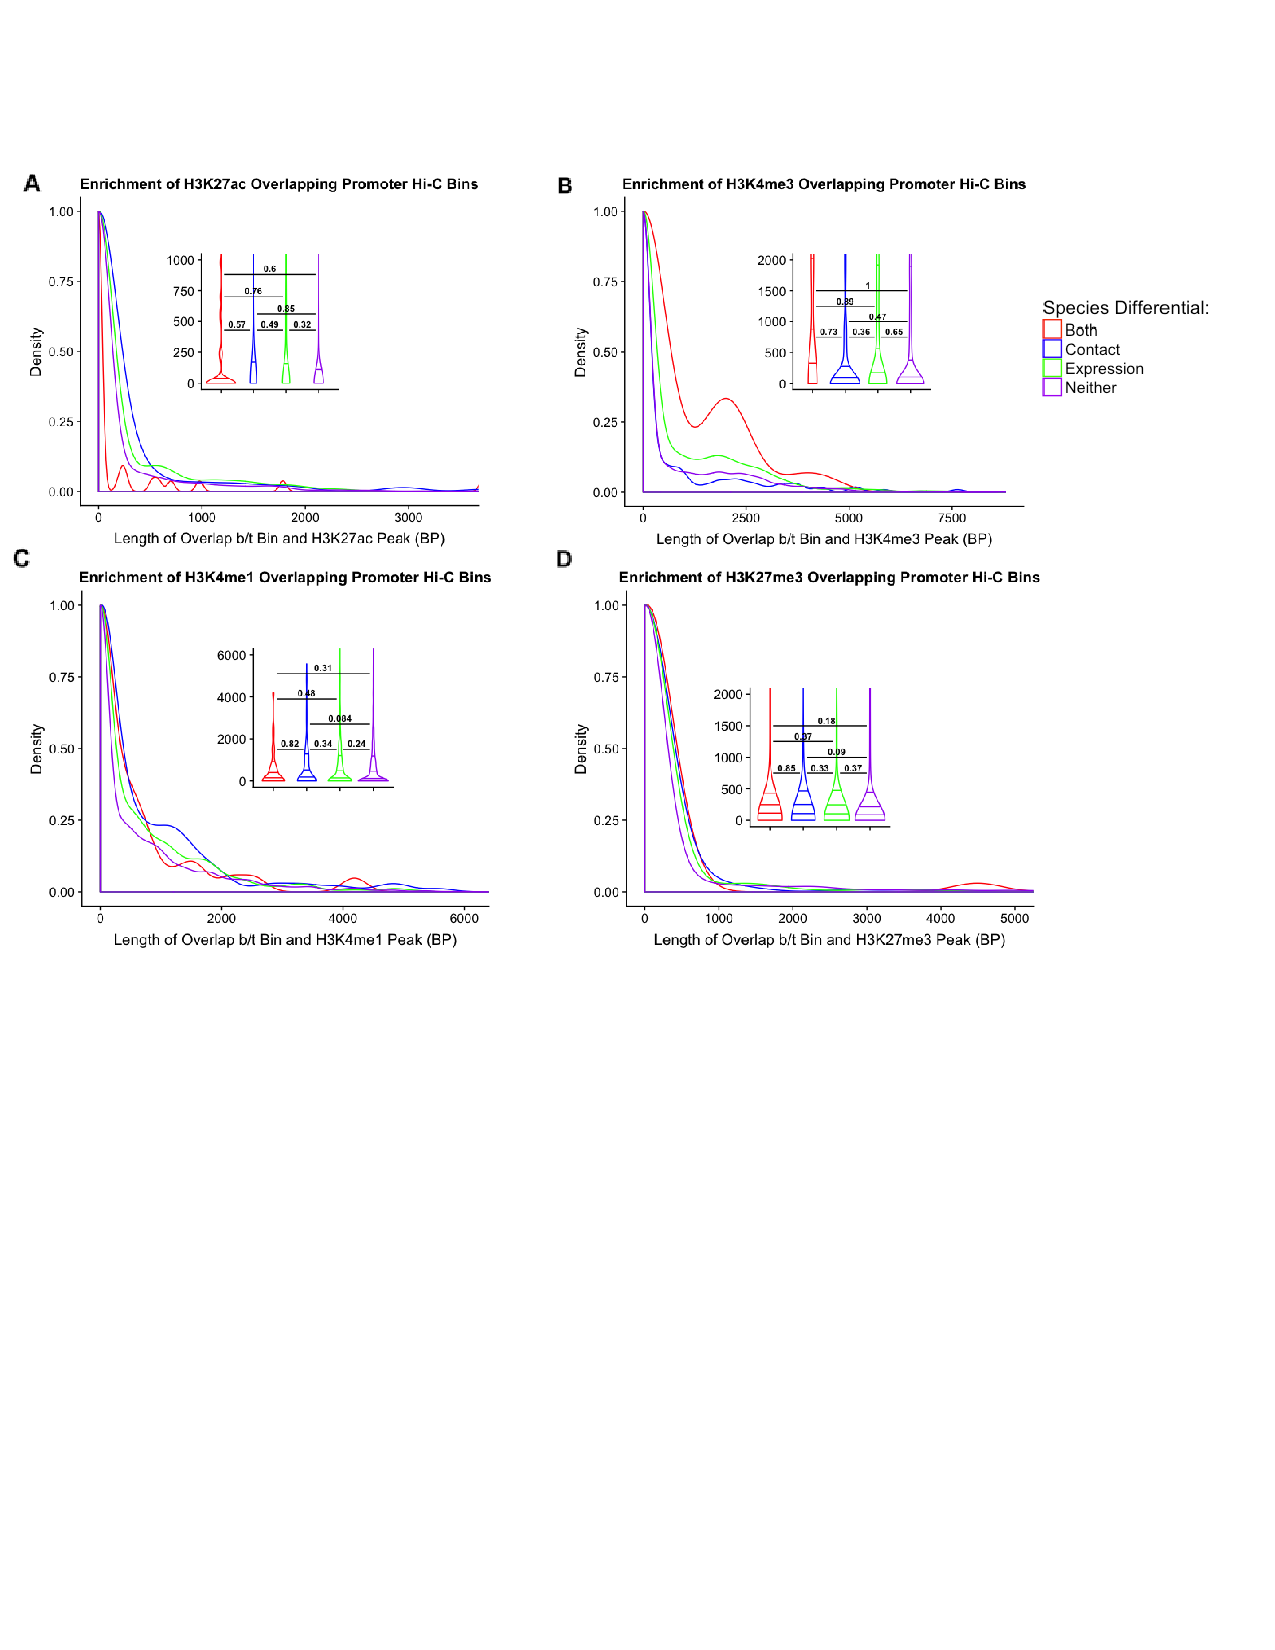
\includegraphics[width=6in]{img/figS5.pdf}
\caption[Overlap of activating and repressive histone marks among Hi-C contacts, Juicer.]{\textbf{S5. Overlap of activating and repressive histone marks among Hi-C contacts, Juicer.} (A) Density plot of the base pair overlap between different classes of Hi-C contact loci and H3K27ac. Histone mark data were obtained from ENCODE in experiments carried out in human iPSCs. We grouped contacts into 4 classes, indicated by color: those that show differential contact between species, those that show differential expression between species, those that show both, and those that show neither. We used pairwise t-tests to compare differences in the mean overlap among the four classes of Hi-C loci. Unlike in the HOMER-normalized data, we do not observe statistically significant differences in overlaps with H3K27ac between different locus classes. This may reflect the previous observation that the hiccups algorithm for assigning statistical significance of loops in Hi-C data is much more conservative than HOMER's significance calling method \cite{Forcato.2017}. (B) Same as A, but performed on H3K4me3 data obtained from ENCODE, collected in hESCs. (C) Same as A and B, but performed on H3K4me1 data obtained from ENCODE, collected in human iPSCs. (D) Same as A, B, and C, but performed on H3K27me3 data obtained from ENCODE, collected in human iPSCs.}
\label{fig:ch02-figS5}
\end{figure}

\begin{figure}[!htb]
\centering
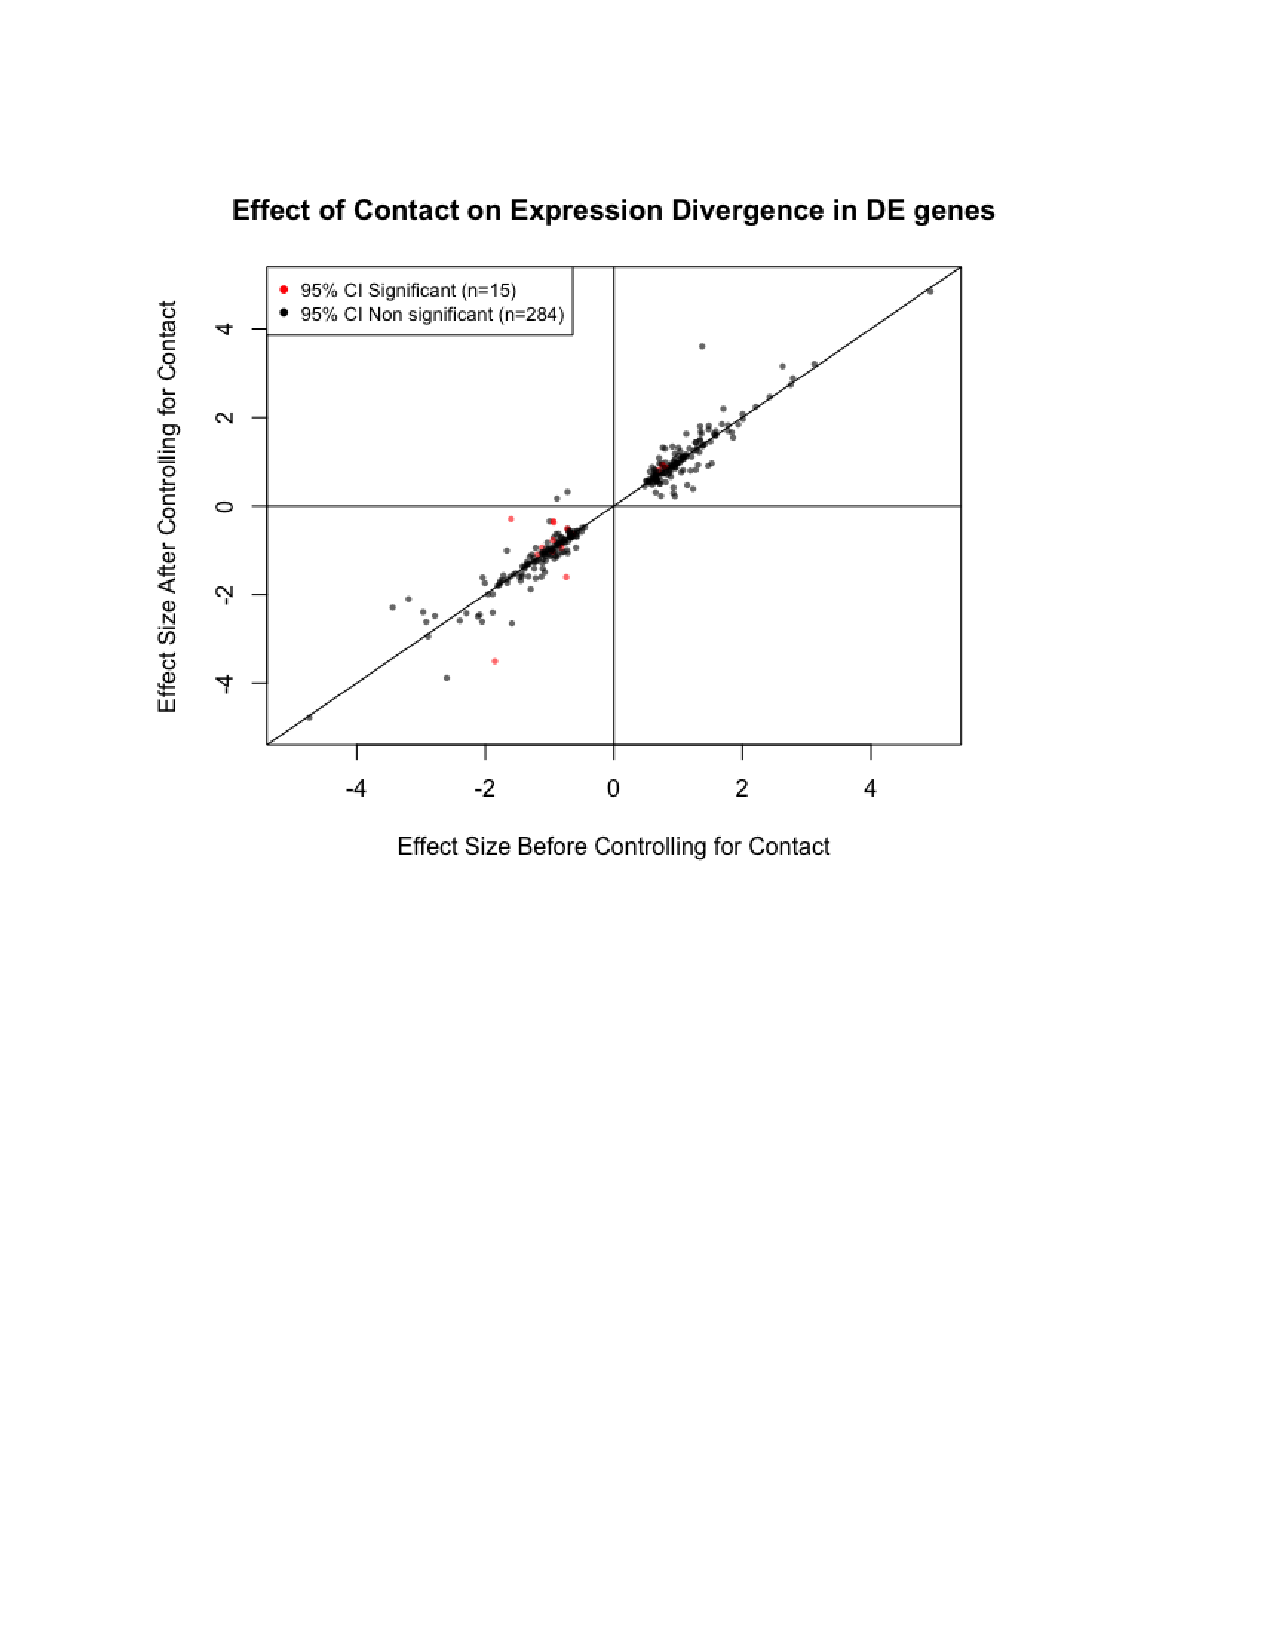
\includegraphics[width=6in]{img/figS6.pdf}
\caption[Gene expression variance is explained by chromatin contacts for 5\% of DE genes, Juicer.]{\textbf{S6. Gene expression variance is explained by chromatin contacts for 5\% of DE genes, Juicer.} Plot of the species effect size in DE genes between models before (x-axis) and after (y-axis) conditioning on contact frequency. The Monte Carlo test of significance was used to construct the 95\% confidence interval and evaluate the significance of the indirect effect (species' effect on expression mediated through contact). Amongst DE genes, 5\% (15/299) of genes showed a statistically significant effect of Hi-C contacts on expression levels (i.e. their 95\% confidence interval does not include zero).}
\label{fig:ch02-figS6}
\end{figure}

\begin{figure}[!htb]
\centering
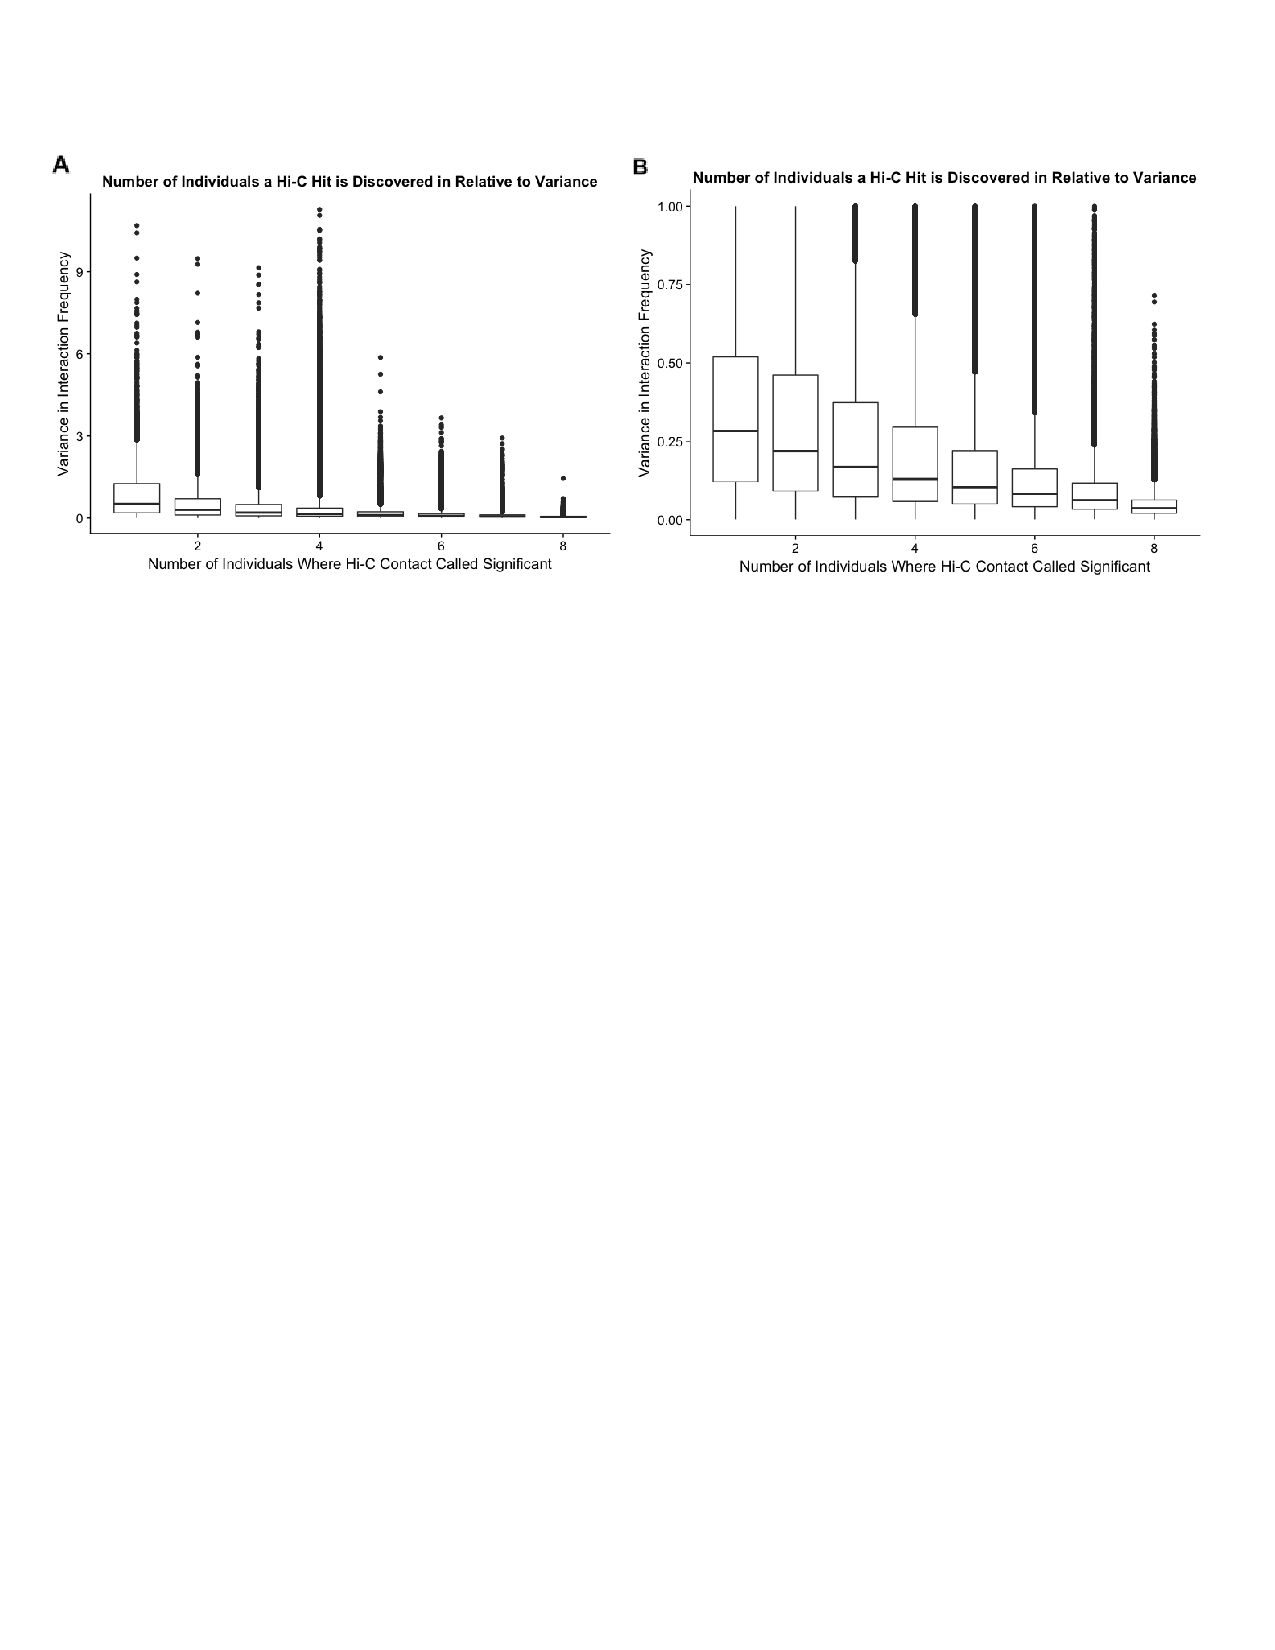
\includegraphics[width=6in]{img/figS7.pdf}
\caption[Variance in interaction frequency as a function of the number of individuals in which a significant interaction is independently discovered.]{\textbf{S7. Variance in interaction frequency as a function of the number of individuals in which a significant interaction is independently discovered.} (A) Boxplots of variance in contact frequency across all 8 individuals on the y-axis, binned by the number of individuals in which an interaction is independently called significant on the x-axis. (B) Same as A, but zoomed in on the y-axis to visualize finer-scale variation.}
\label{fig:ch02-figS7}
\end{figure}

\begin{figure}[!htb]
\centering
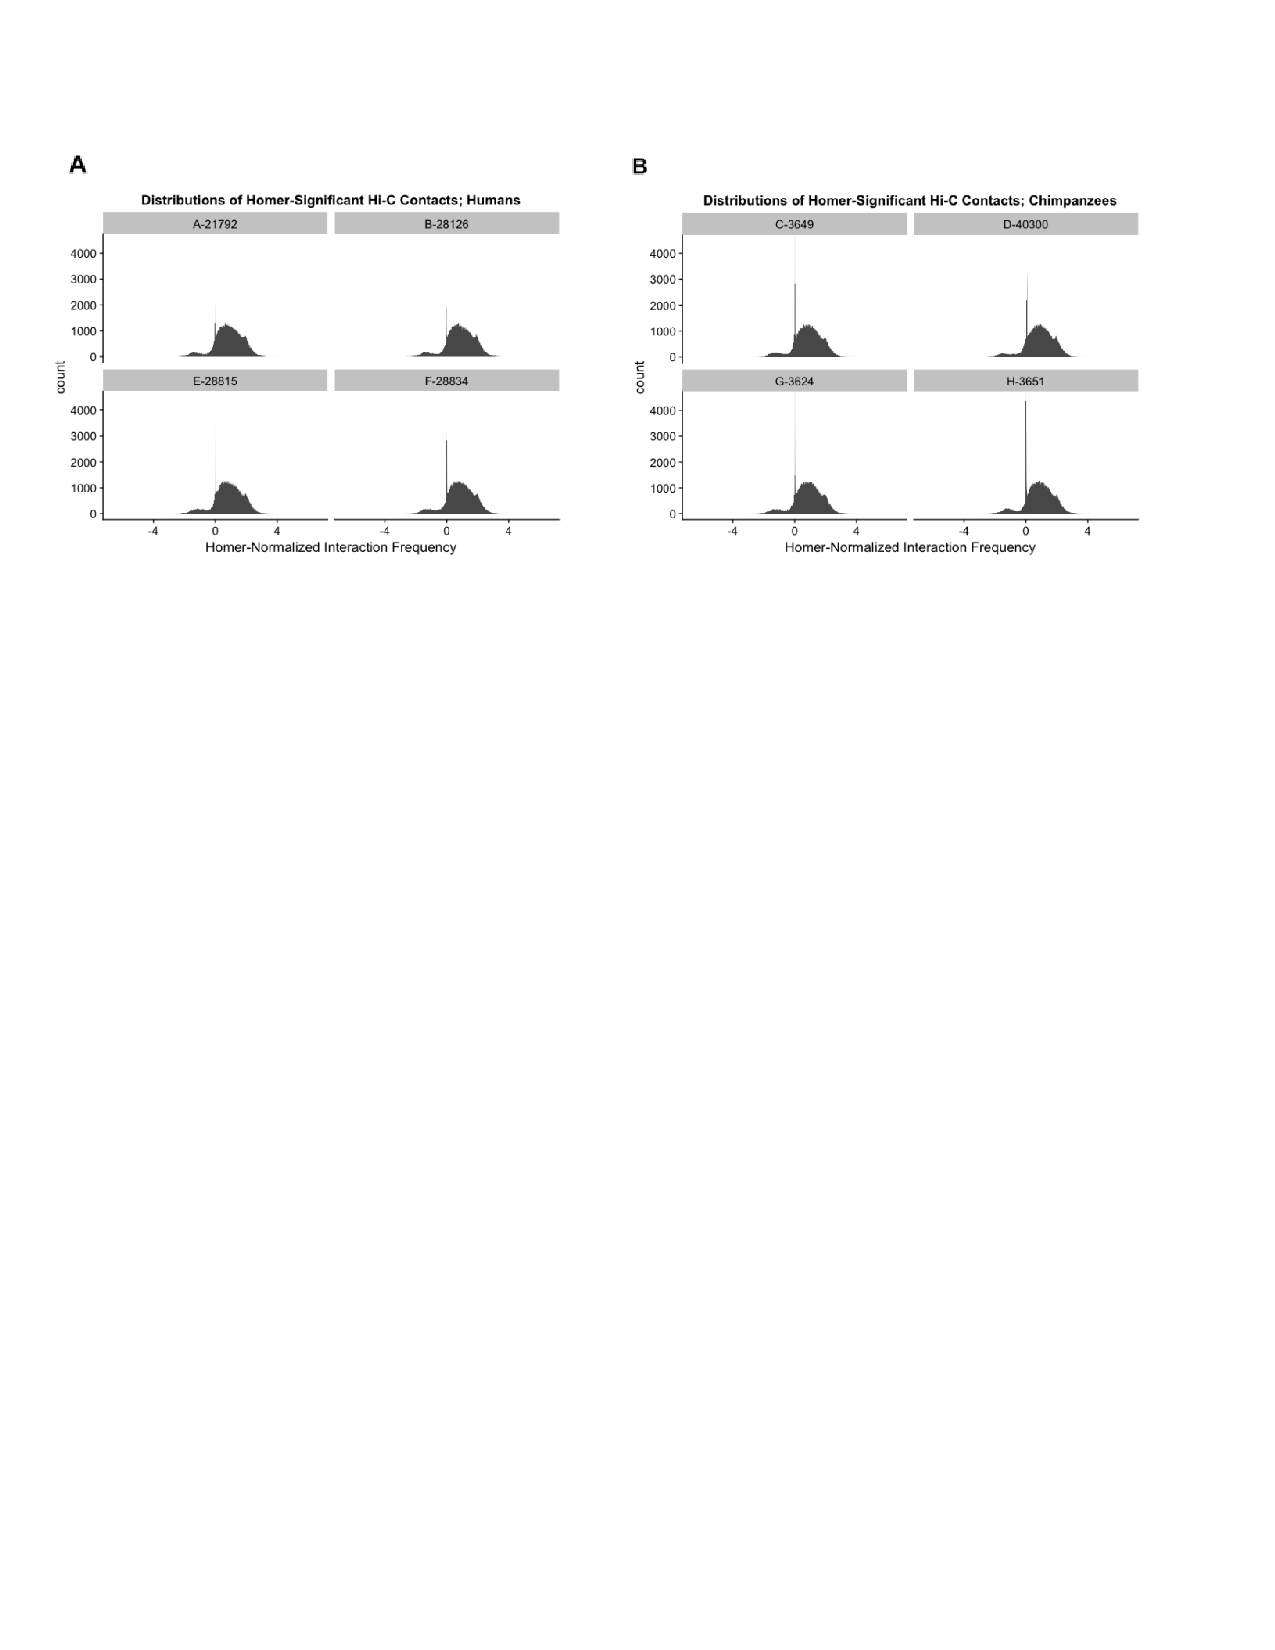
\includegraphics[width=6in]{img/figS8.pdf}
\caption[Distributions of HOMER-normalized interaction frequencies are remarkably similar across species.]{\textbf{S8. Distributions of HOMER-normalized interaction frequencies are remarkably similar across species.} (A) Histogram of log\textsubscript{2}(observed/expected) HOMER-normalized interaction frequencies in all four human samples used in this study, after applying pairwise cyclic loess normalization with limma \cite{Smyth.2004}. (B) Same as A, but in chimpanzees.}
\label{fig:ch02-figS8}
\end{figure}

\begin{figure}[!htb]
\centering
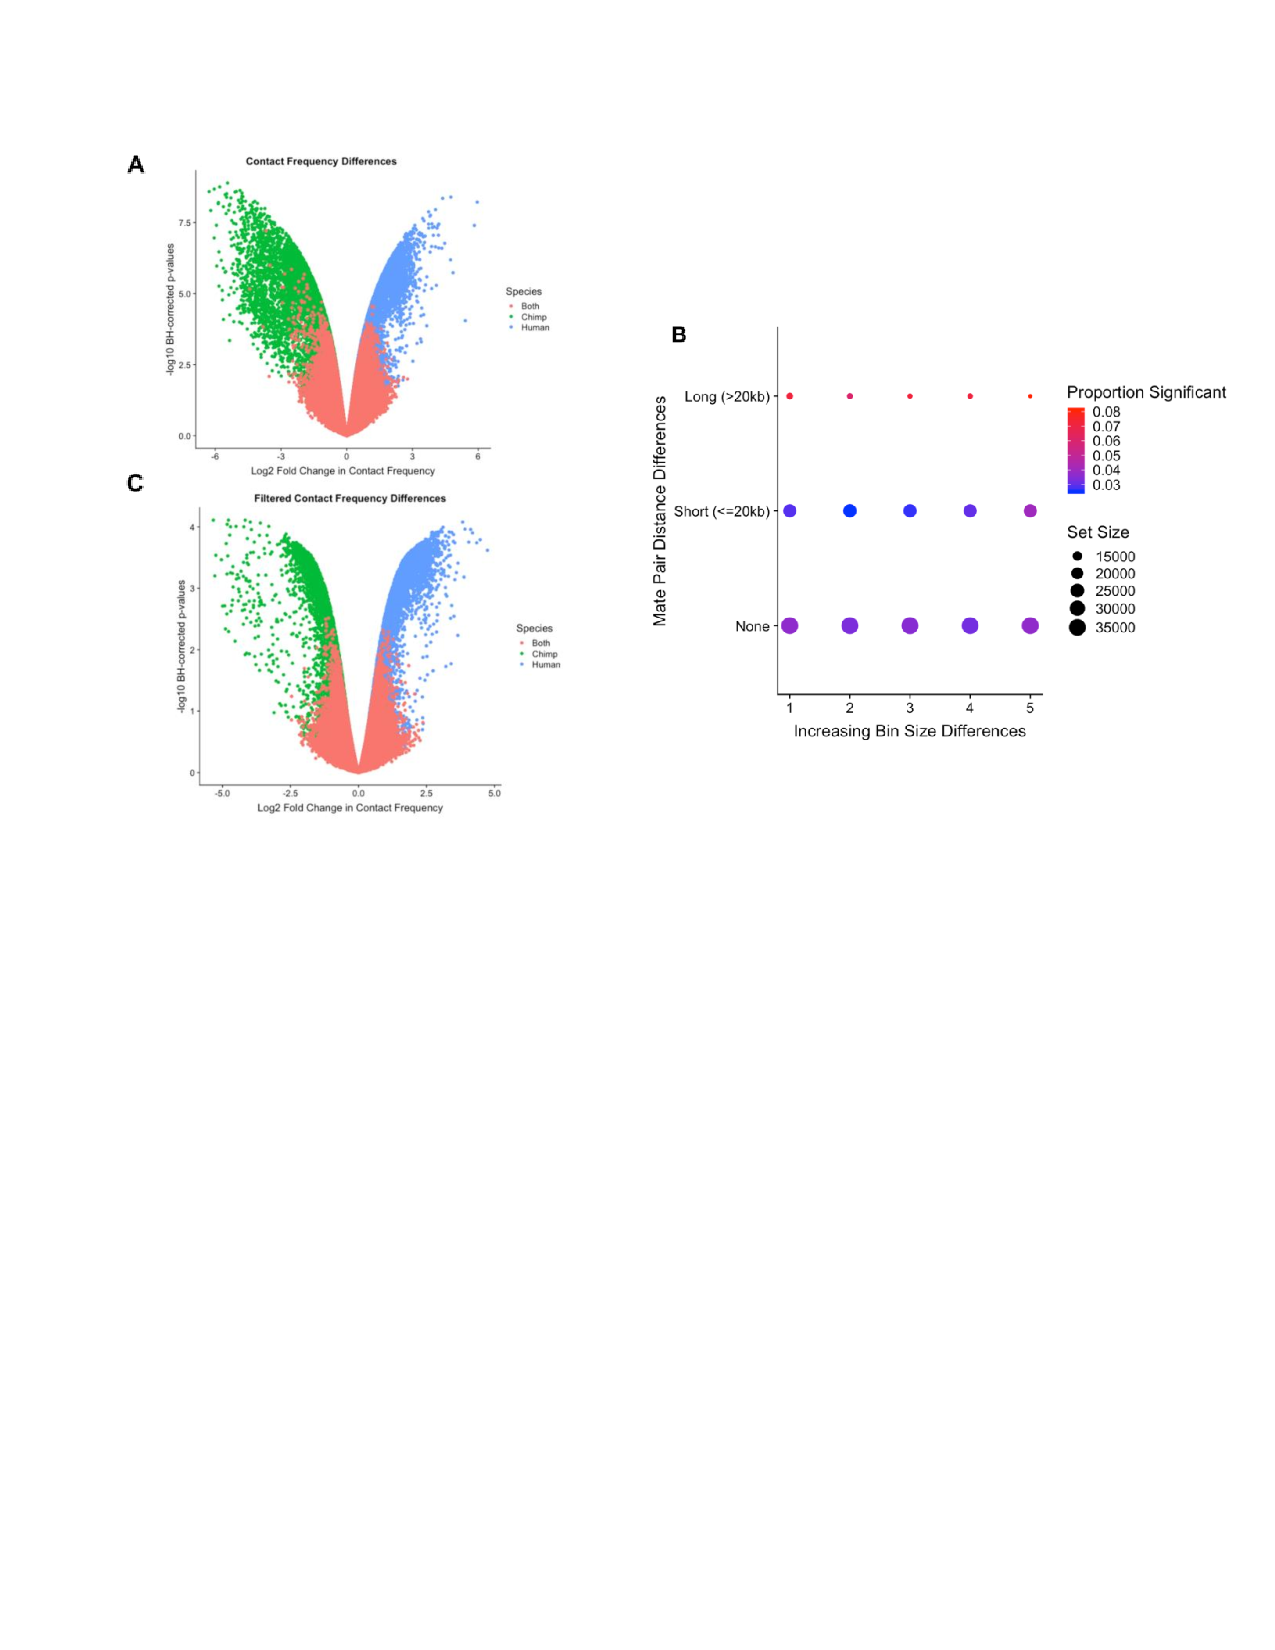
\includegraphics[width=6in]{img/figS9.pdf}
\caption[Volcano plot asymmetry quality control.]{\textbf{S9. Volcano plot asymmetry quality control.} (A) Volcano plot of log\textsubscript{2} fold change in contact frequency between humans and chimpanzees (x-axis) against Benjamini-Hochberg FDR (y-axis). This plot shows data only filtered for independent discovery in at least 4 individuals. Data are colored by the species in which the contact was originally identified as significant. (B) Scatter plot of sets of Hi-C contacts, with proportion of contacts significant in our linear modeling of interaction frequency shown based on color. Contacts are binned by mate-pair distance differences (y-axis) and bin size differences (x-axis). Circle size is proportional to the size of the set of Hi-C contacts falling into each criteria. Red indicates that the data were filtered out after this step, and blue/purple indicates that the data were retained for further analysis. (C) Volcano plot as in A, but after removing contacts with large mate-pair distance differences across the species.}
\label{fig:ch02-figS9}
\end{figure}

\begin{figure}[!htb]
\centering
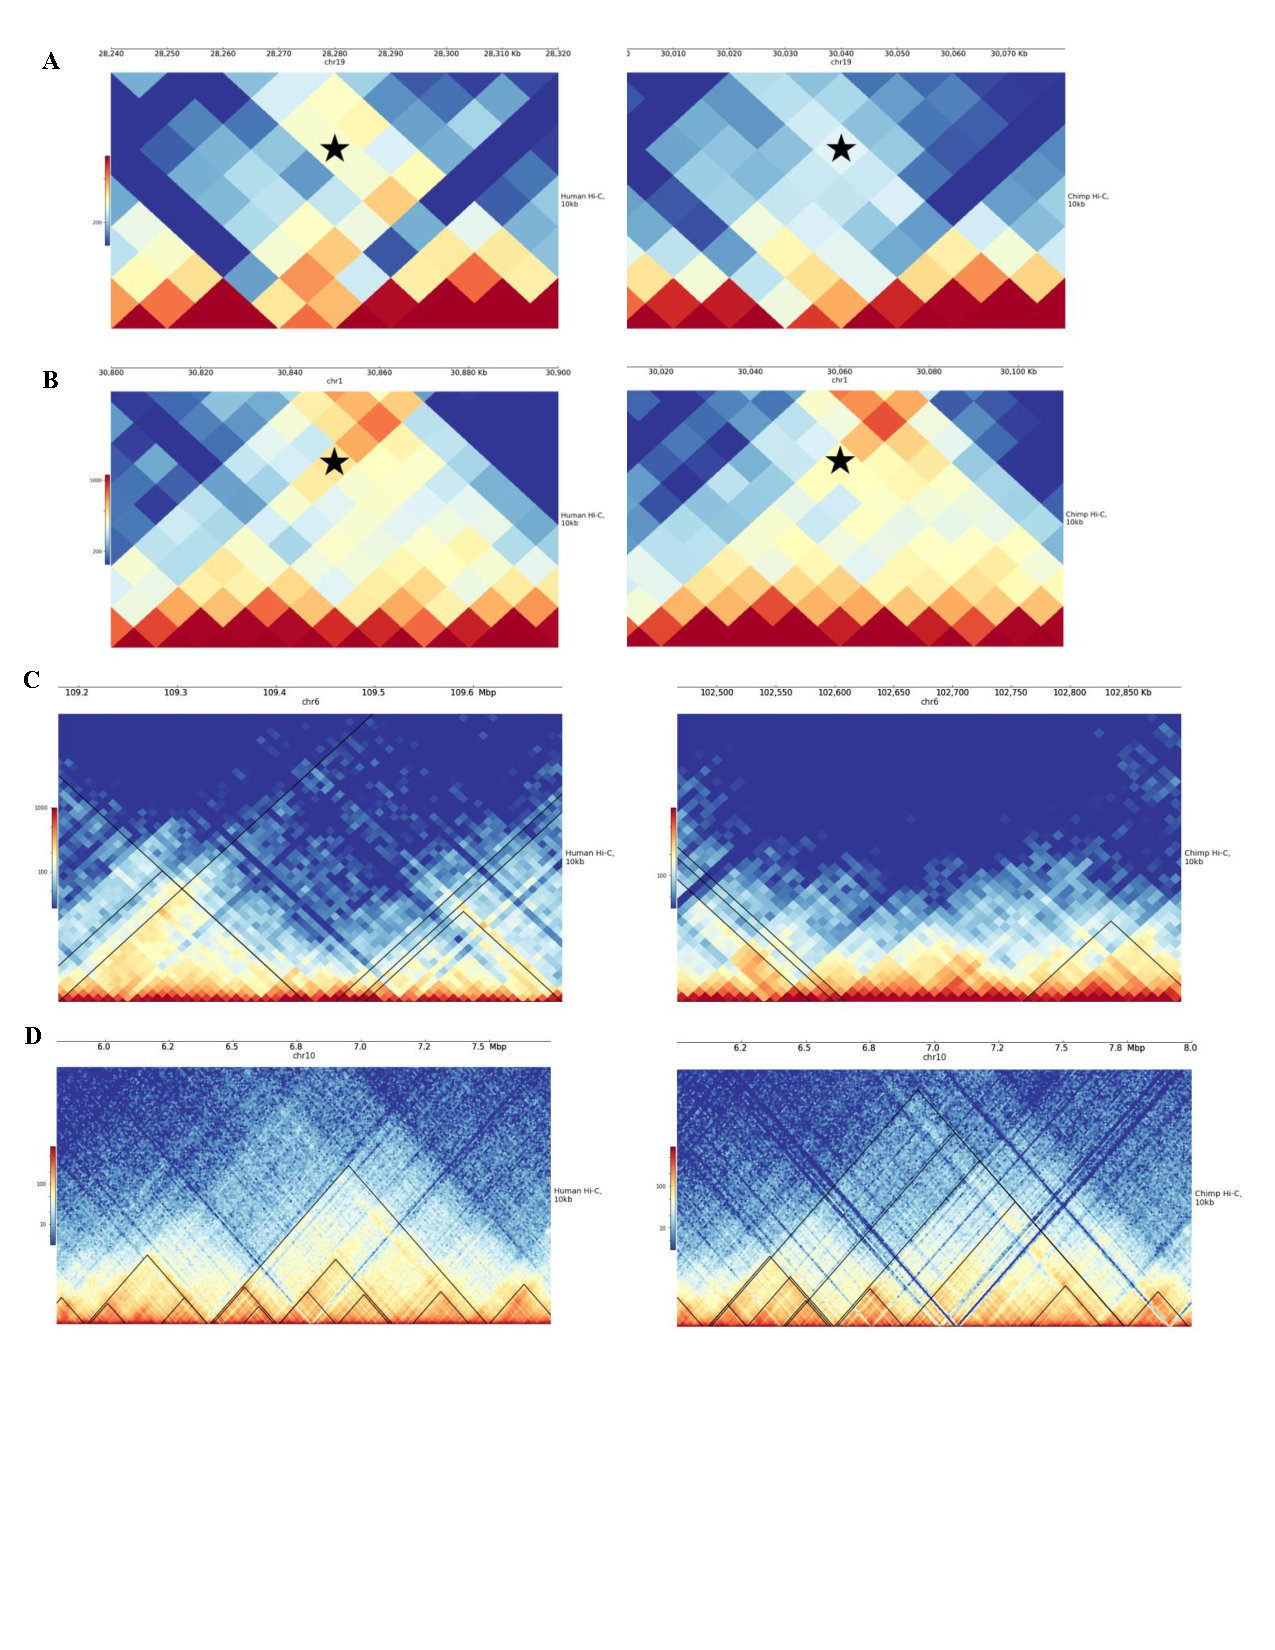
\includegraphics[width=6in]{img/figS10.1.pdf}
\caption[Further visual examples of DC and non-DC interactions; conserved and divergent TADs.]{\textbf{S10. Further visual examples of DC and non-DC interactions; conserved and divergent TADs.} (A) PyGenomeTracks plots \cite{Ramirez.2018} of a chromosome 19 interaction between bins 80 kb away for human (left panel) and chimpanzee (right panel). The bin pair tested is indicated by a black star, and was found to be DC between species. (B) Same as A, but for a conserved (non-DC) interaction on chromosome 1 separated by 100kb. (continued on next page)}
\label{fig:ch02-figS10}
\end{figure}

\begin{figure}[!htb]
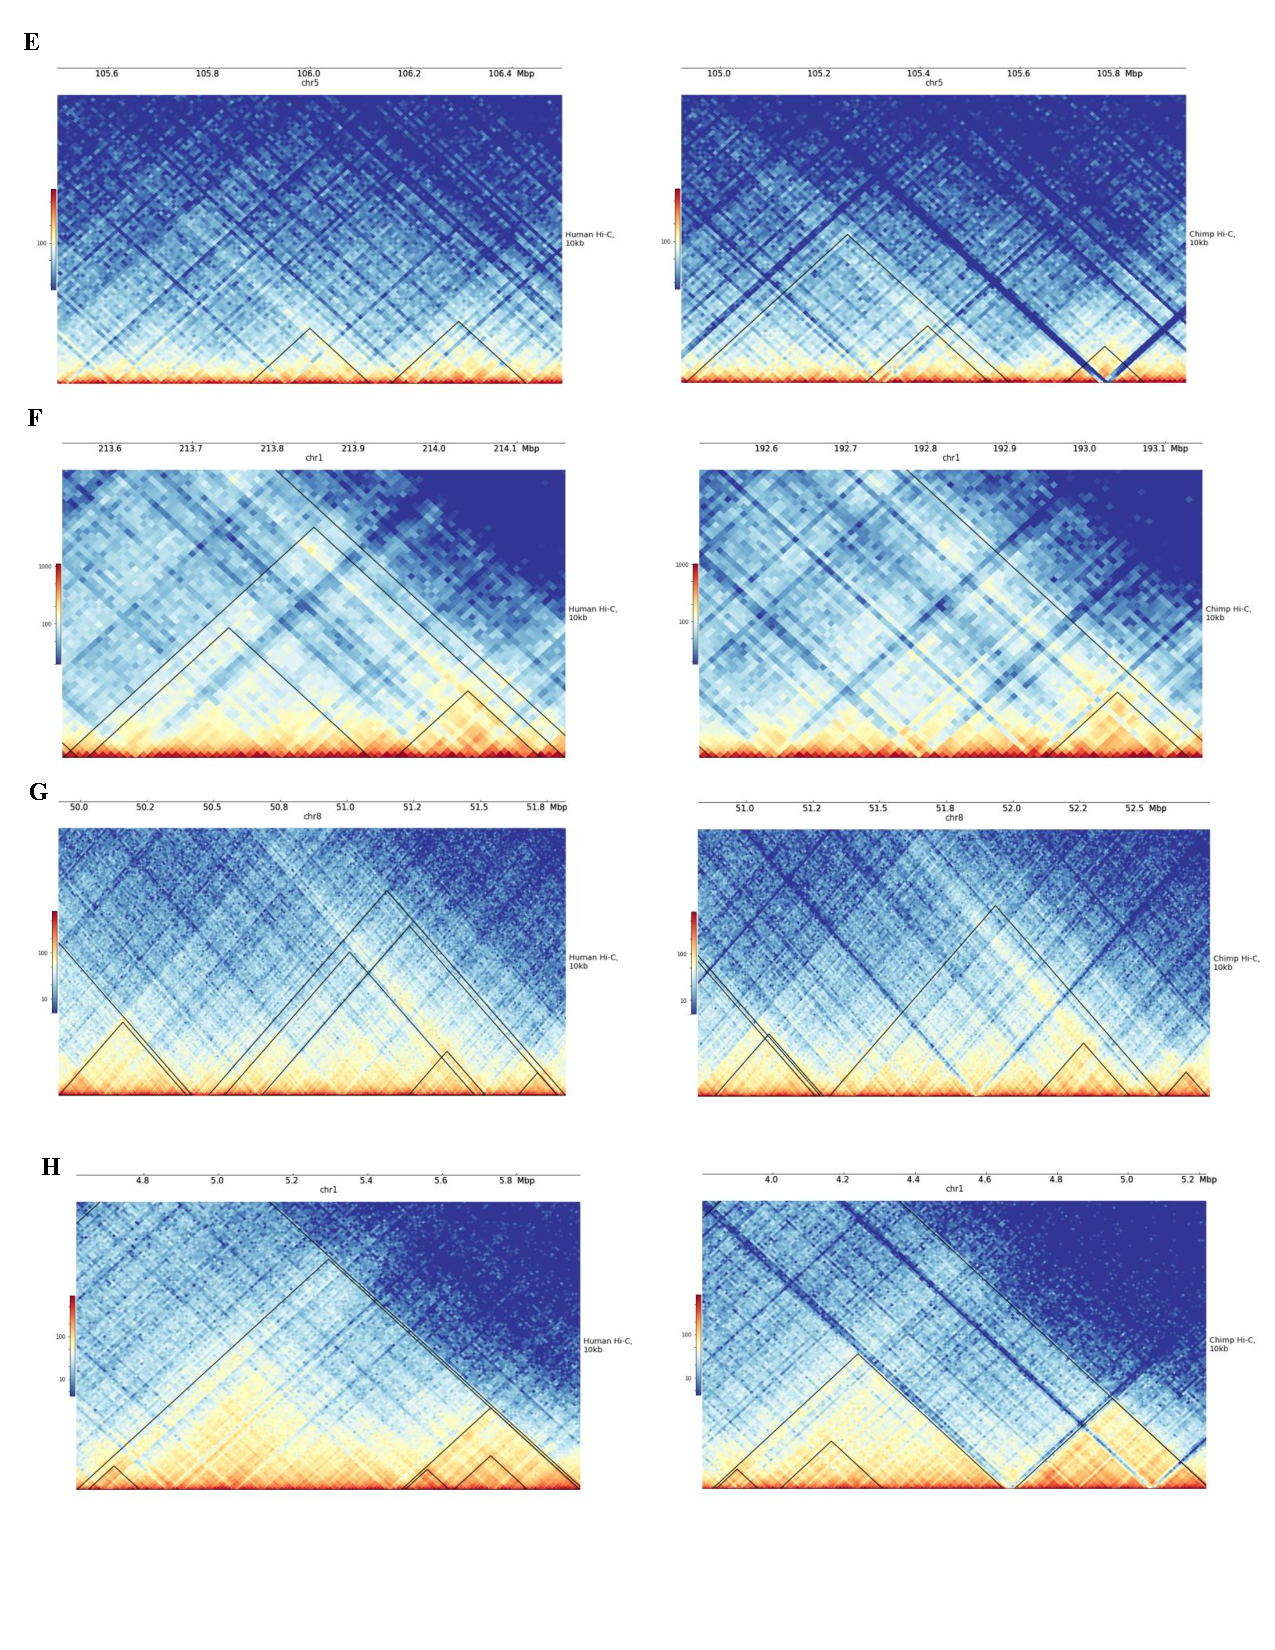
\includegraphics[width=6in]{img/figS10.2.pdf}
\contcaption{(C-H) Examples of contact maps (created with PyGenomeTracks \cite{Ramirez.2018}) and Arrowhead-inferred TAD structures (black lines) in humans (left) and chimpanzees (right), across a number of different chromosomes. In most examples, inference based on the algorithm indicates shared and species-specific domains, yet these are difficult to ascertain based on visual inspection, as discussed.}
\end{figure}

\begin{figure}[!htb]
\centering
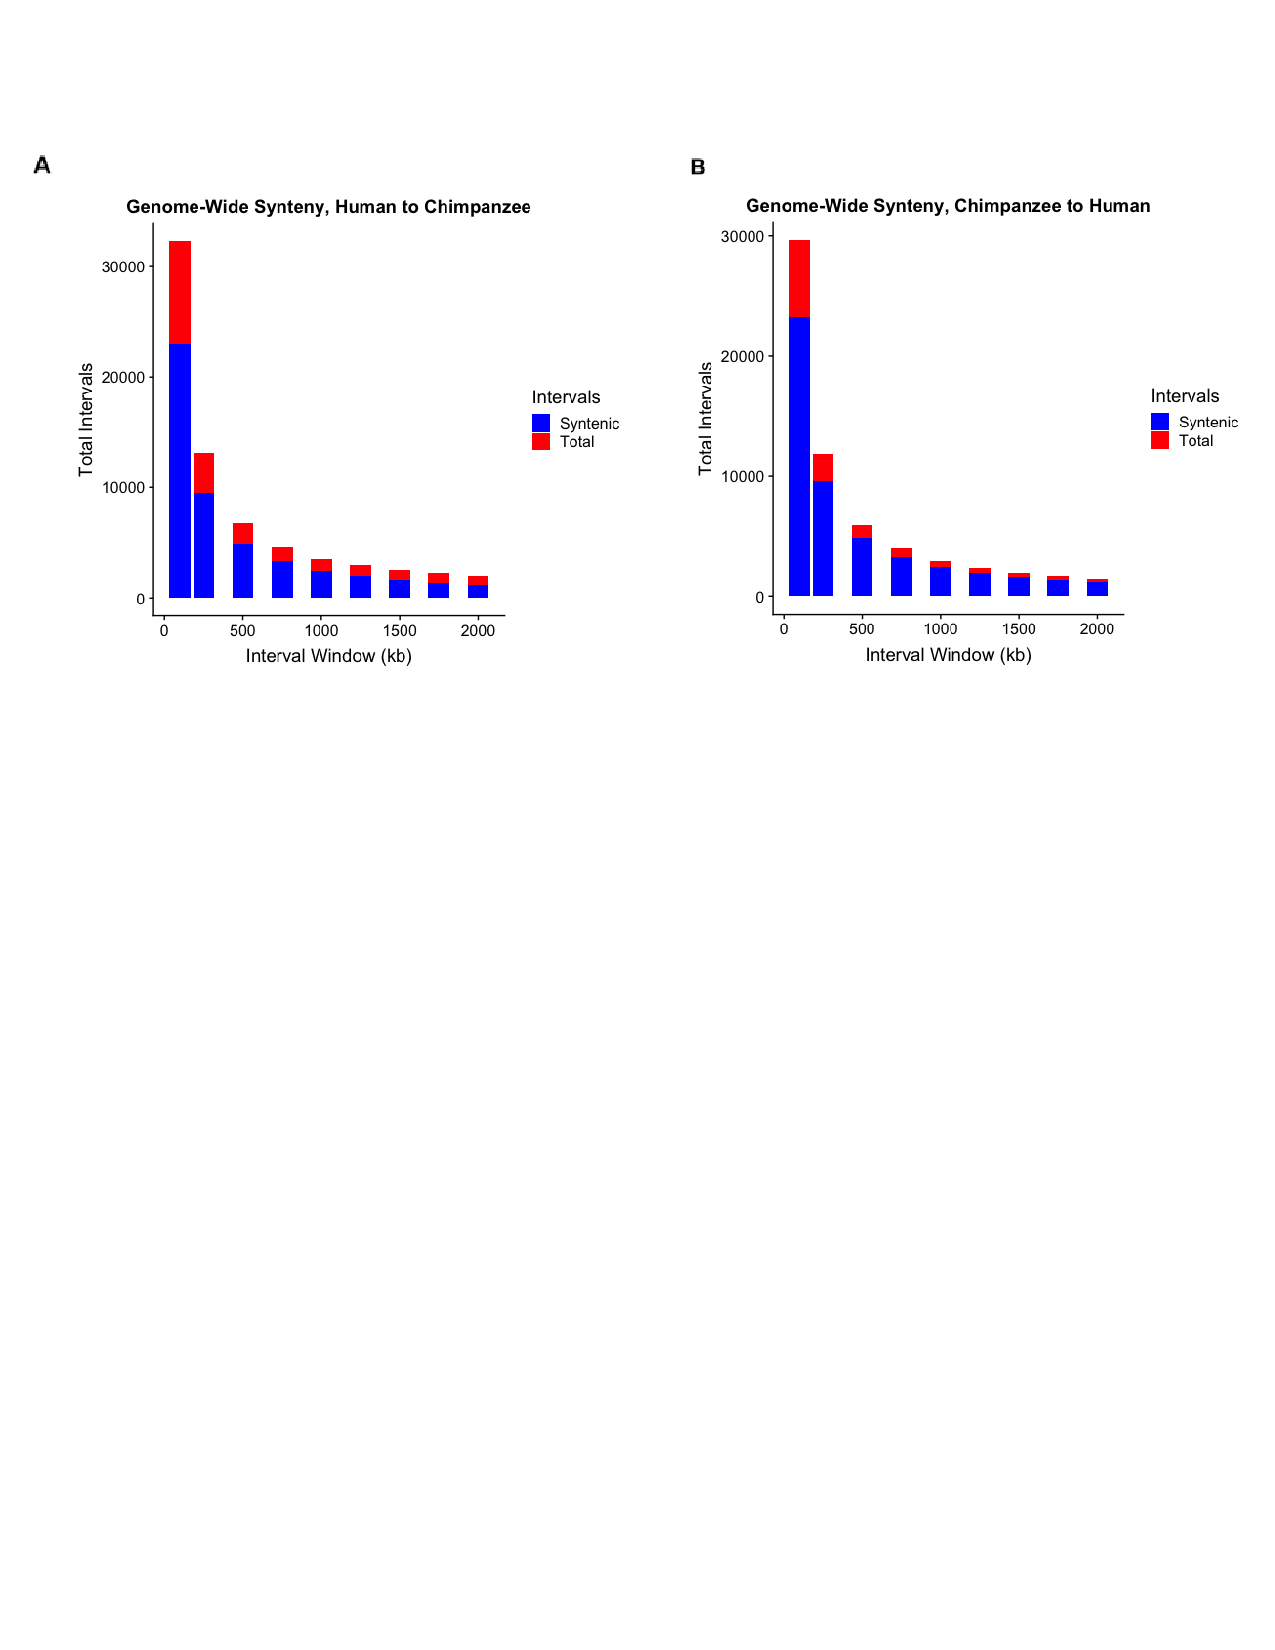
\includegraphics[width=6in]{img/figS11.pdf}
\caption[Synteny of large scale linear genomic intervals between human and chimpanzee.]{\textbf{S11. Synteny of large scale linear genomic intervals between human and chimpanzee.} (A) Across different window sizes (x-axis) for a genome-wide tiling of hg38, we plotted the number of total and syntenic linear intervals (y-axis), identified using the reciprocal best hits liftOver method \cite{Ward.2014, Kent.2002} we employed throughout the paper. (B) Same as A, but for a genome-wide tiling of panTro5.}
\label{fig:ch02-figS11}
\end{figure}

\begin{figure}[!htb]
\centering
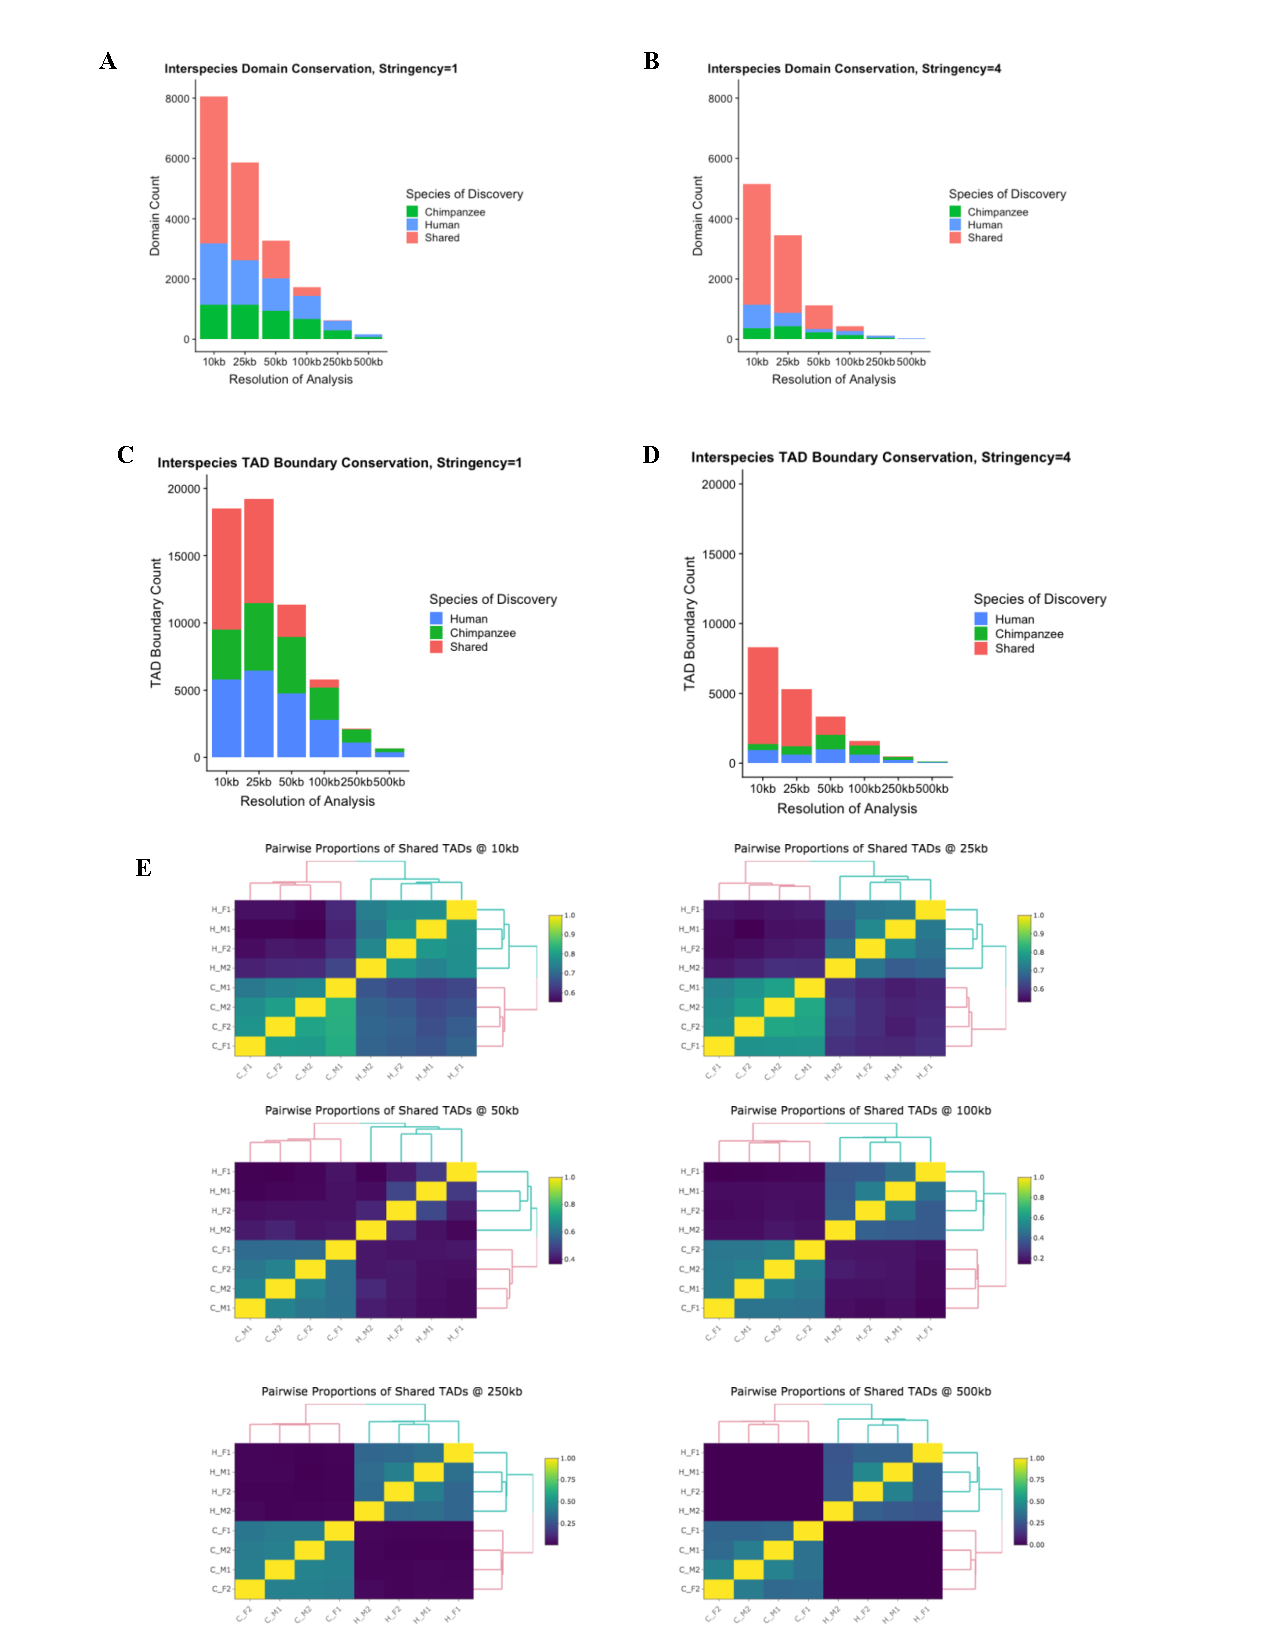
\includegraphics[width=4in]{img/figS12.1.pdf}
\caption[Higher-order chromosomal structure in humans and chimpanzees with alternative analysis choices.]{\textbf{S12. Higher-order chromosomal structure in humans and chimpanzees with alternative analysis choices.} (A) Across different resolutions (x-axis), we plotted the number of shared and species-specific domains (y-axis) identified with Arrowhead \cite{Durand.2016} on Juicer VC-normalized Hi-C maps from each individual. We called domain conservation here based on the method of Rao et al. \cite{Rao.2014} (highly similar results were observed with our 90\% reciprocal overlap method, described in the text and available in the github repository associated with the paper). (continued on next page)}
\label{fig:ch02-figS12}
\end{figure}

\begin{figure}[!htb]
\centering
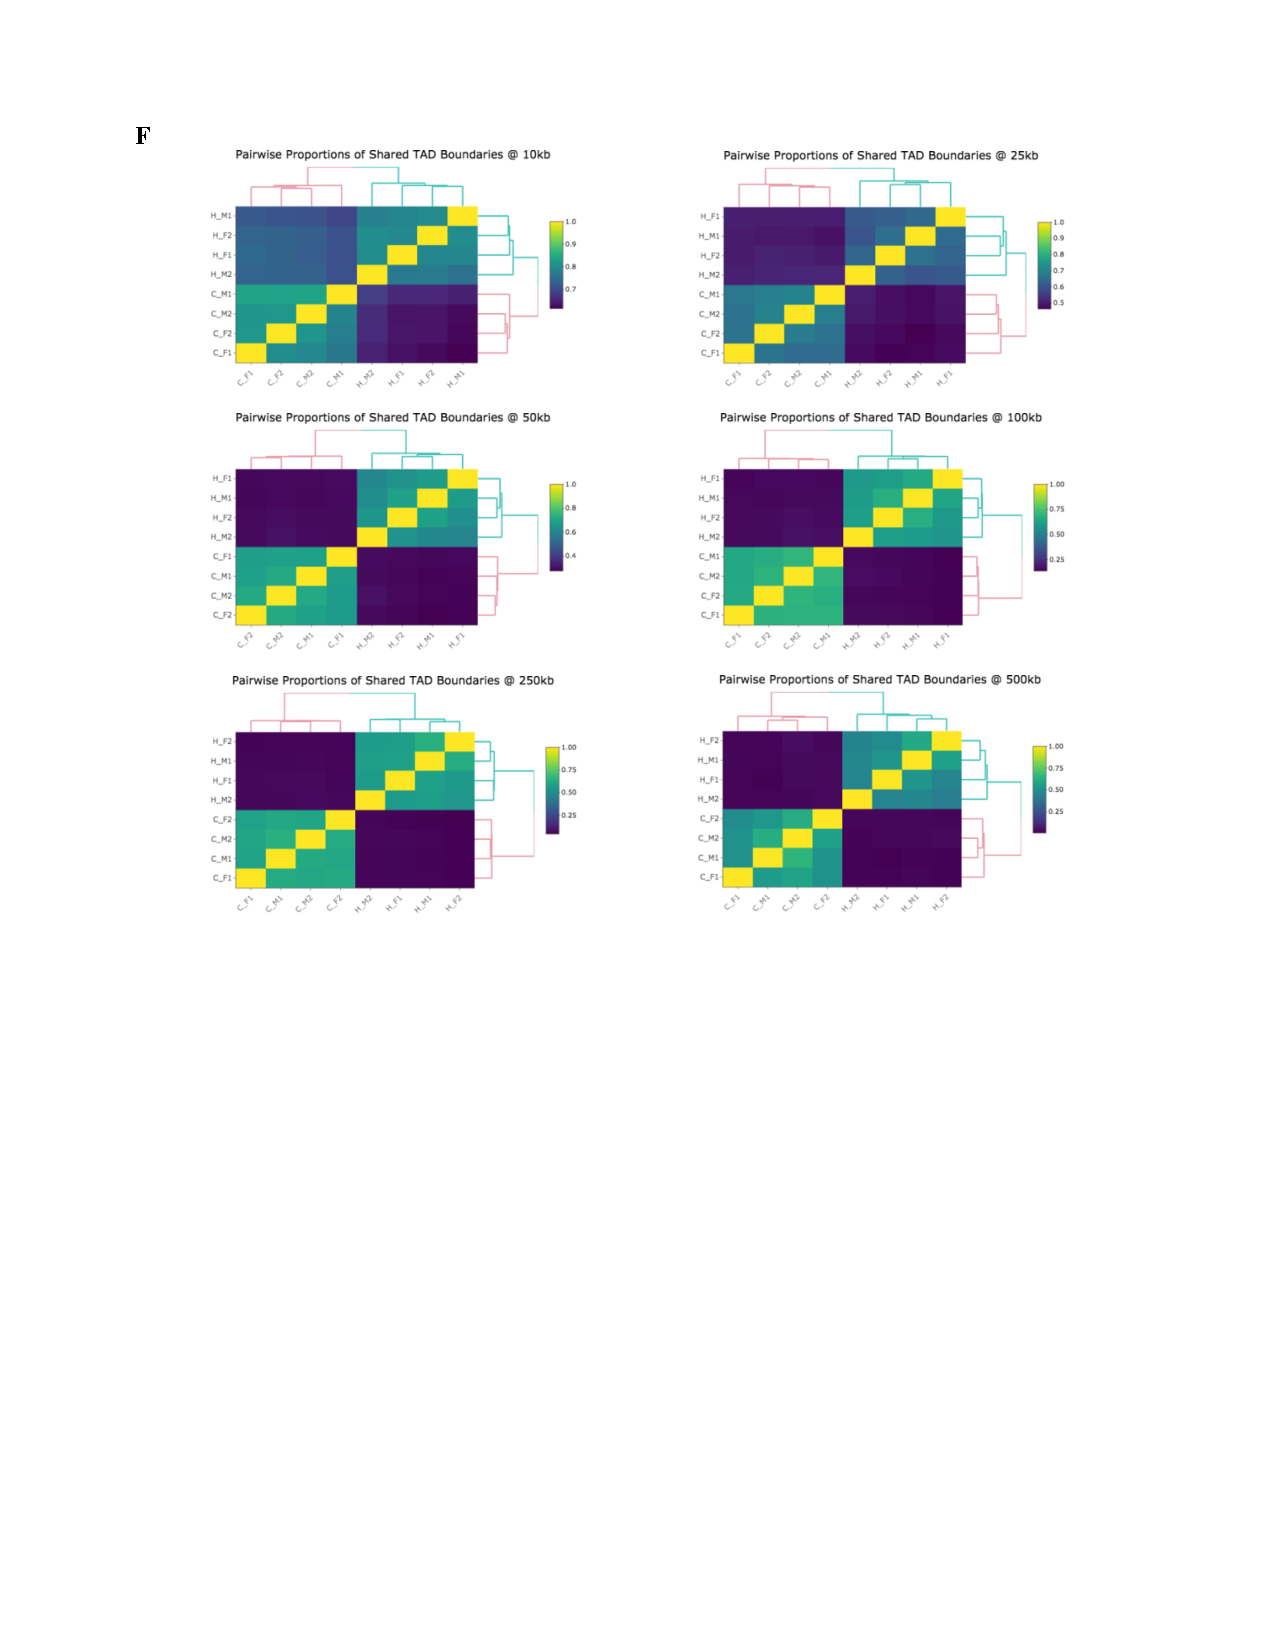
\includegraphics[width=4in]{img/figS12.2.pdf}
\contcaption{Domain count values represent the average interspecies sharing across all individuals, with no filtering for domain robustness (that is, assessing all domains discovered and orthologously mappable). Under this analysis paradigm we observe relatively low sharing across species ($\sim$60\% at 10kb). (B) Same as A, but this time, only considering TADs that were found across all 4 individuals within either one of the species (fixed TADs). Restricting to this subset increases the percentage of conservation to 78\%, although the set of TADs being examined is much smaller. (C) Same as A, but for boundaries instead of domains. Boundaries were defined as 15kb flanking regions at the edges of inferred Arrowhead domains. Because the TADs called by Arrowhead are nested, we merged boundaries here to obtain unique genomic intervals, rather than counting boundaries repeatedly. We then considered boundaries shared between individuals if they had any overlap. (D) Same as B, but for boundaries instead of domains (i.e. considering only boundaries fixed within species). Here, the highest estimate of conservation we obtain is 83\% of boundaries conserved across species at 10kb resolution. (E) Unsupervised hierarchical clustering of the pairwise proportions of shared TADs between all individuals in our study at a variety of resolutions, using the Rao et al. \cite{Rao.2014} methodology for calling conservation. The first letter in the labels demarcates the species (H for human and C for chimpanzee), and the following symbols indicate sex (male, M or female, F) and batch (1 or 2). Heatmaps are not necessarily symmetric because different numbers of TADs were discovered in different individuals; rows represent an individual's shared proportion of TADs (individual total) with each other individual. Highly similar clustering results were observed when using our domain conservation calling paradigm (shown in github repository associated with paper). (F) Same as E, but for boundaries instead of domains.}
\end{figure}

\begin{figure}[!htb]
\centering
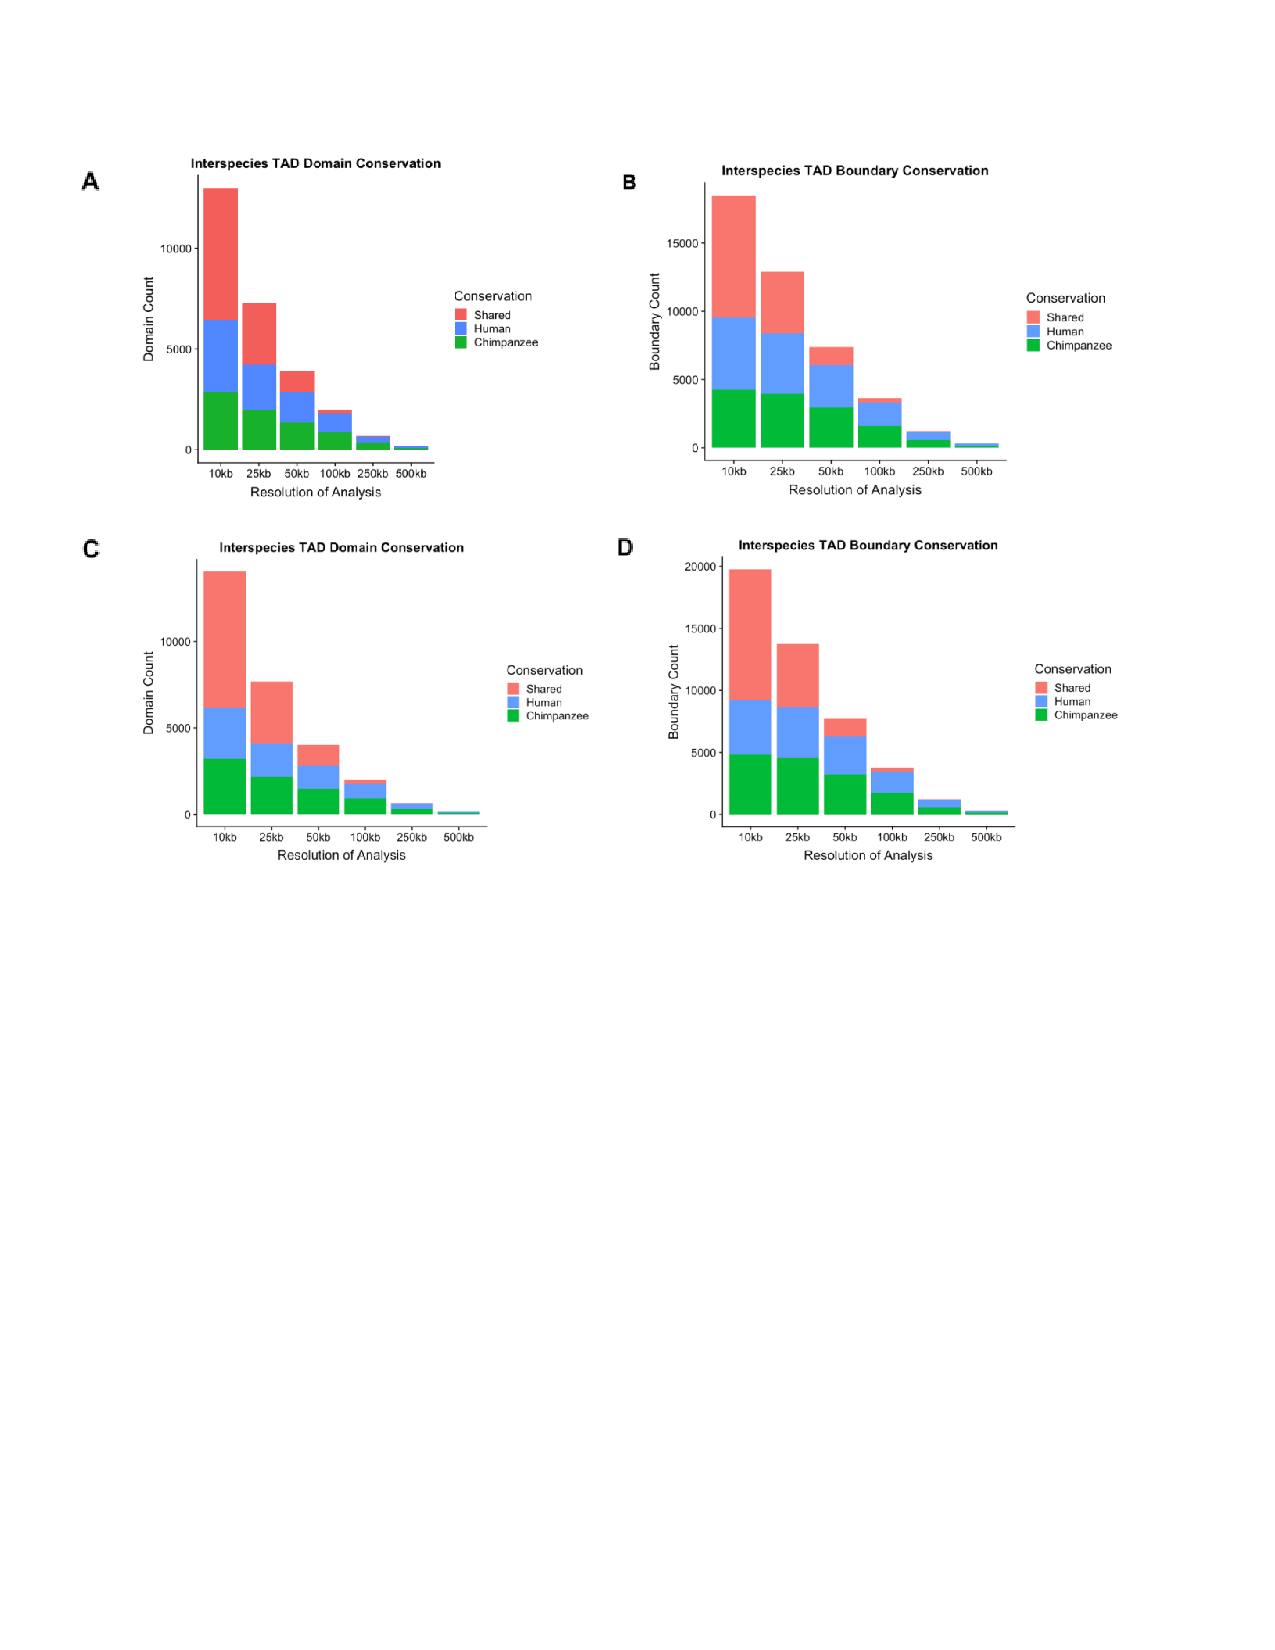
\includegraphics[width=6in]{img/figS13.pdf}
\caption[Higher-order chromosomal structure in humans and chimpanzees with alternative analysis choices and genome builds.]{\textbf{S13. Higher-order chromosomal structure in humans and chimpanzees with alternative analysis choices and genome builds.} (A) Across different resolutions (x-axis), we plotted the number of shared and species-specific domains (y-axis) identified with Arrowhead \cite{Durand.2016} using the consensus map from each species. To call a domain as conserved here, we required that the Euclidean distance between the domain across species be less than the minimum of 50kb or 50\% the length of the TAD, based on the conservation calling method employed by Rao et al \cite{Rao.2014}. Results are highly similar to those seen in Fig 4A. (B) Same as A, but for TAD boundaries instead of the domains themselves. Boundaries were defined as 15 kb flanking regions at the edges of inferred Arrowhead domains. In this case, conservation was called if there was any base pair overlap between boundaries. Unlike in Fig 4B, boundaries were merged before calling conservation, in order to find unique boundary elements. This difference in analysis paradigms could have important consequences with a nested TAD caller such as Arrowhead \cite{Durand.2016}, but results are highly similar to those seen in Fig 4B. (C) Same as A, but this time, performed on `high-density consensus' Hi-C maps that have been mapped to the hg38 and panTro6 genomes (rather than panTro5). Results are highly similar despite the improvement in genome quality build. (D) Same as B, but this time, on the hg38 and panTro6 genome assemblies.}
\label{fig:ch02-figS13}
\end{figure}

\begin{figure}[!htb]
\centering
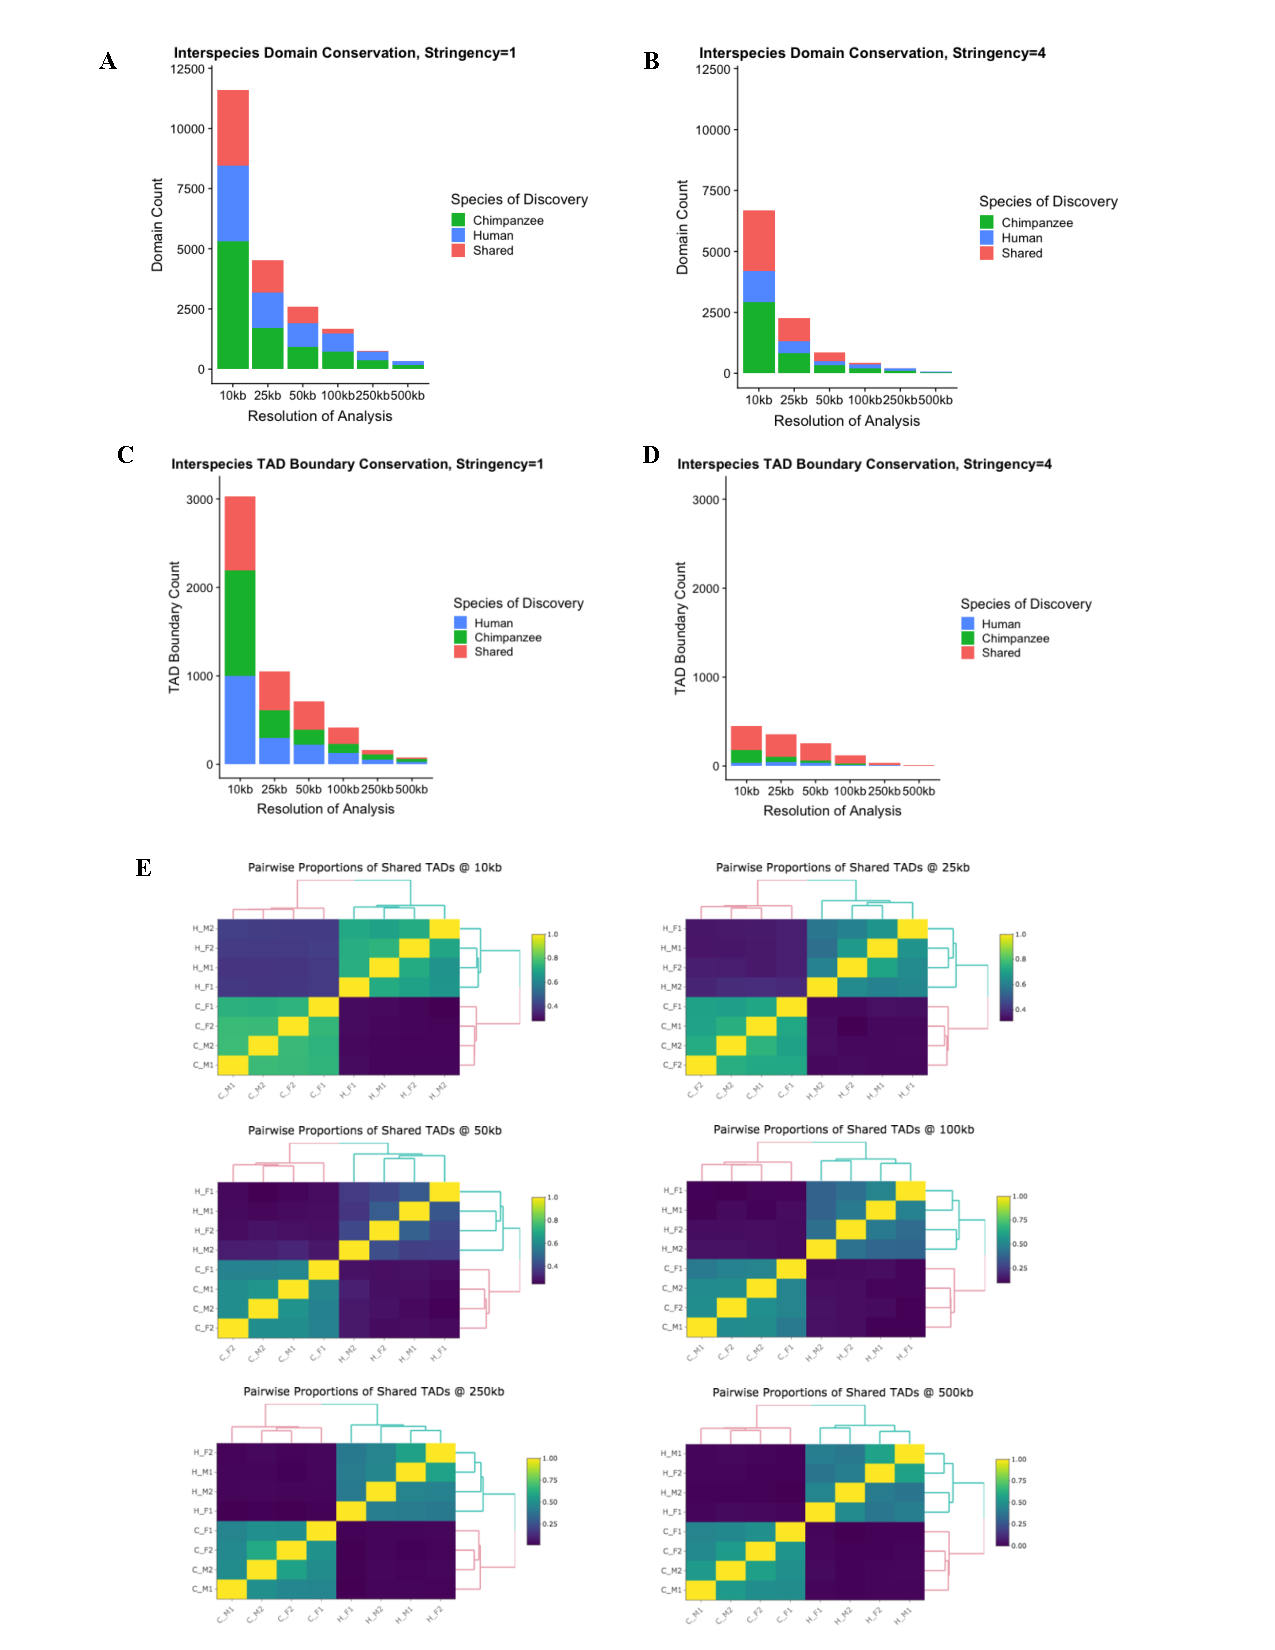
\includegraphics[width=4in]{img/figS14.1.pdf}
\caption[Higher-order chromosomal structure in humans and chimpanzees with alternative algorithms (TopDom).]{\textbf{S14. Higher-order chromosomal structure in humans and chimpanzees with alternative algorithms (TopDom).} (A) Across different resolutions (x-axis), we plotted the number of shared and species-specific domains (y-axis) identified with TopDom \cite{Shin.2016} on HOMER-normalized Hi-C maps from each individual. We called domain conservation here based on the method of Rao et al. \cite{Rao.2014} (highly similar results were observed with our 90\% reciprocal overlap method, described in the text and available in the github repository associated with the paper). (continued on next page)}
\label{fig:ch02-figS14}
\end{figure}

\begin{figure}[!htb]
\centering
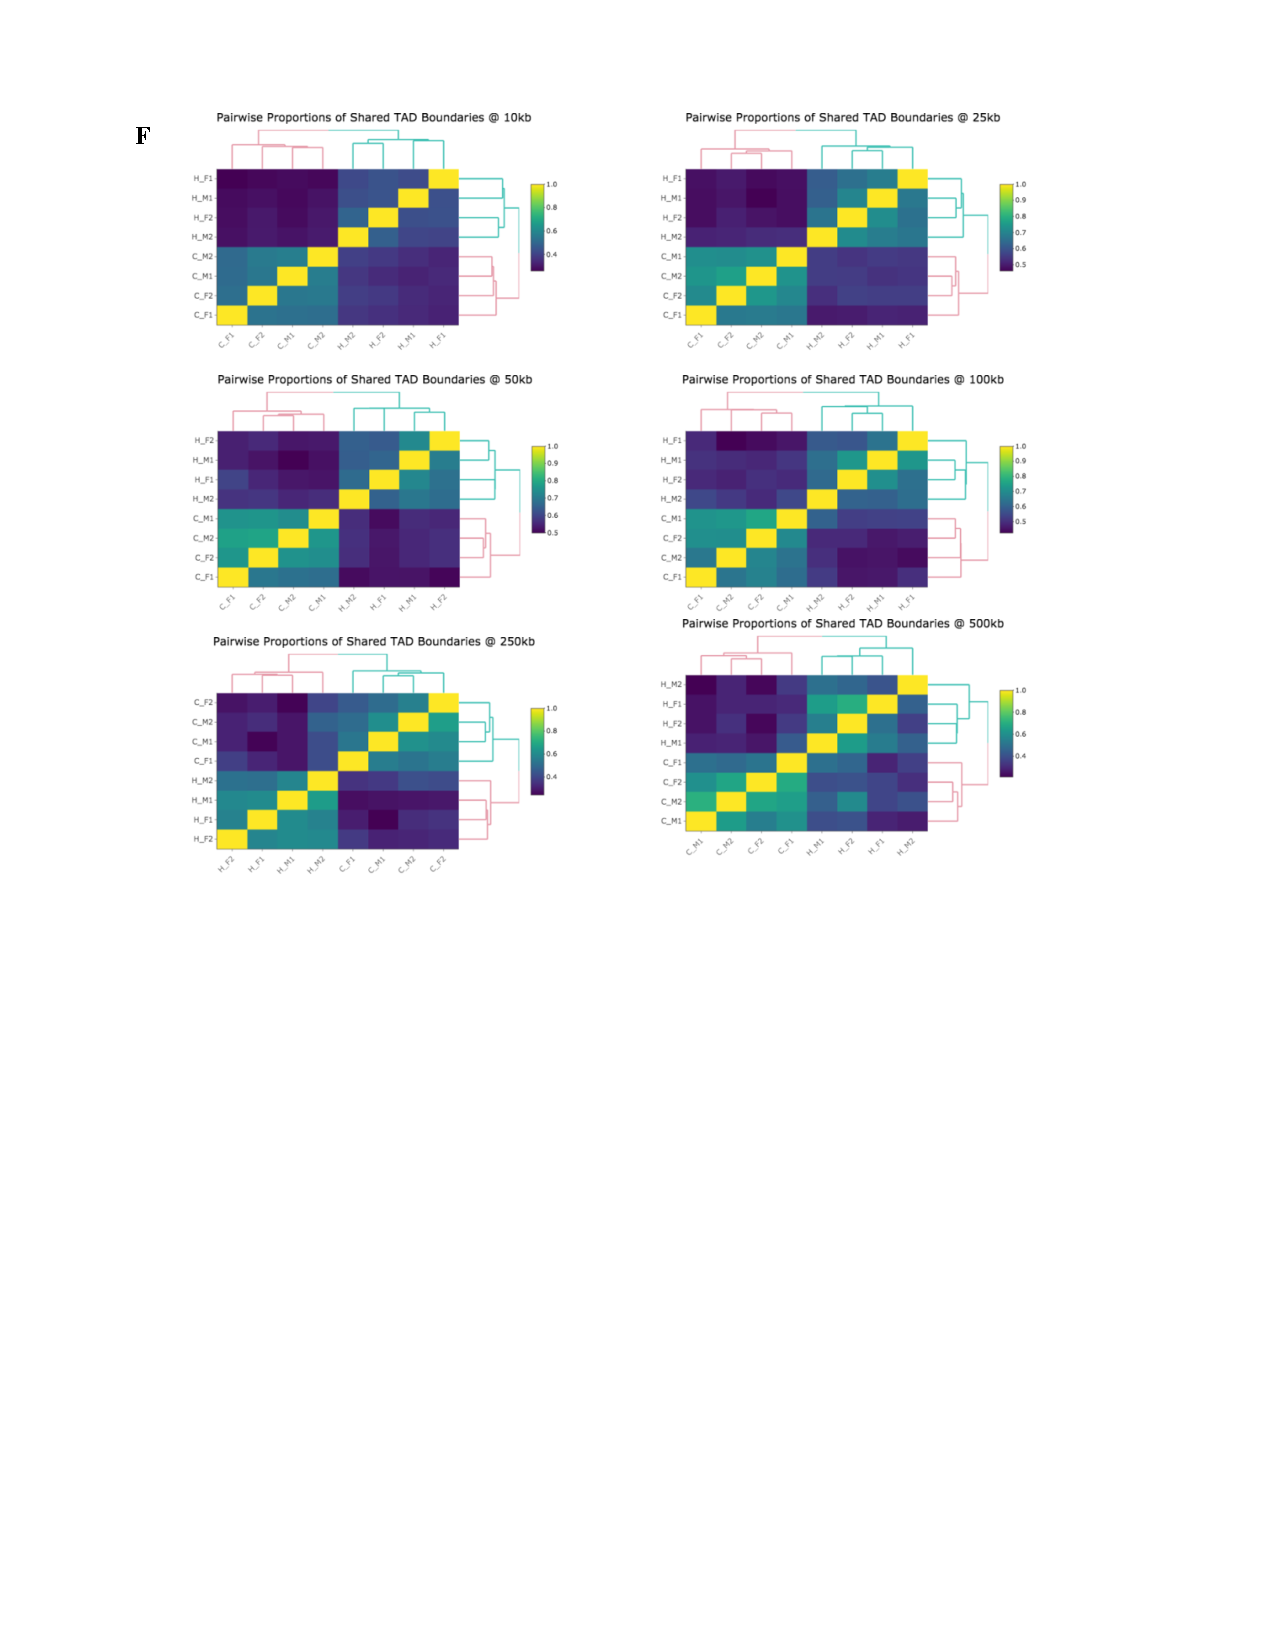
\includegraphics[width=4in]{img/figS14.2.pdf}
\contcaption{Domain count values represent the average interspecies sharing across all individuals, with no filtering for domain robustness (that is, assessing all domains discovered and orthologously mappable). Under this analysis paradigm we observe relatively low sharing across species (maximum of 30\% at 25 kb). (B) Same as A, but this time, only considering TADs that were found across all 4 individuals within either one of the species (fixed TADs). Restricting to this subset increases the maximum percentage of conservation to 42\% at 25 kb resolution, although the set of TADs being examined is much smaller. (C) Same as A, but for TopDom \cite{Shin.2016} boundary inferences instead of domains. We considered boundaries shared between individuals if they had any overlap. (D) Same as B, but for boundaries instead of domains (i.e. considering only boundaries fixed within species). Here, the highest estimate of conservation we obtain is 76\% of boundaries conserved across species at 50 kb resolution. (E) Unsupervised hierarchical clustering of the pairwise proportions of shared TADs between all individuals in our study at a variety of resolutions, using the Rao et al. \cite{Rao.2014} methodology for calling conservation. The first letter in the labels demarcates the species (H for human and C for chimpanzee), and the following symbols indicate sex (male, M or female, F) and batch (1 or 2). Heatmaps are not necessarily symmetric because different numbers of TADs were discovered in different individuals; rows represent an individual's shared proportion of TADs (individual total) with each other individual. Highly similar clustering results were observed when using our domain conservation calling paradigm (shown in github repository associated with paper). (F) Same as E, but for boundaries instead of domains.}
\end{figure}

\begin{figure}[!htb]
\centering
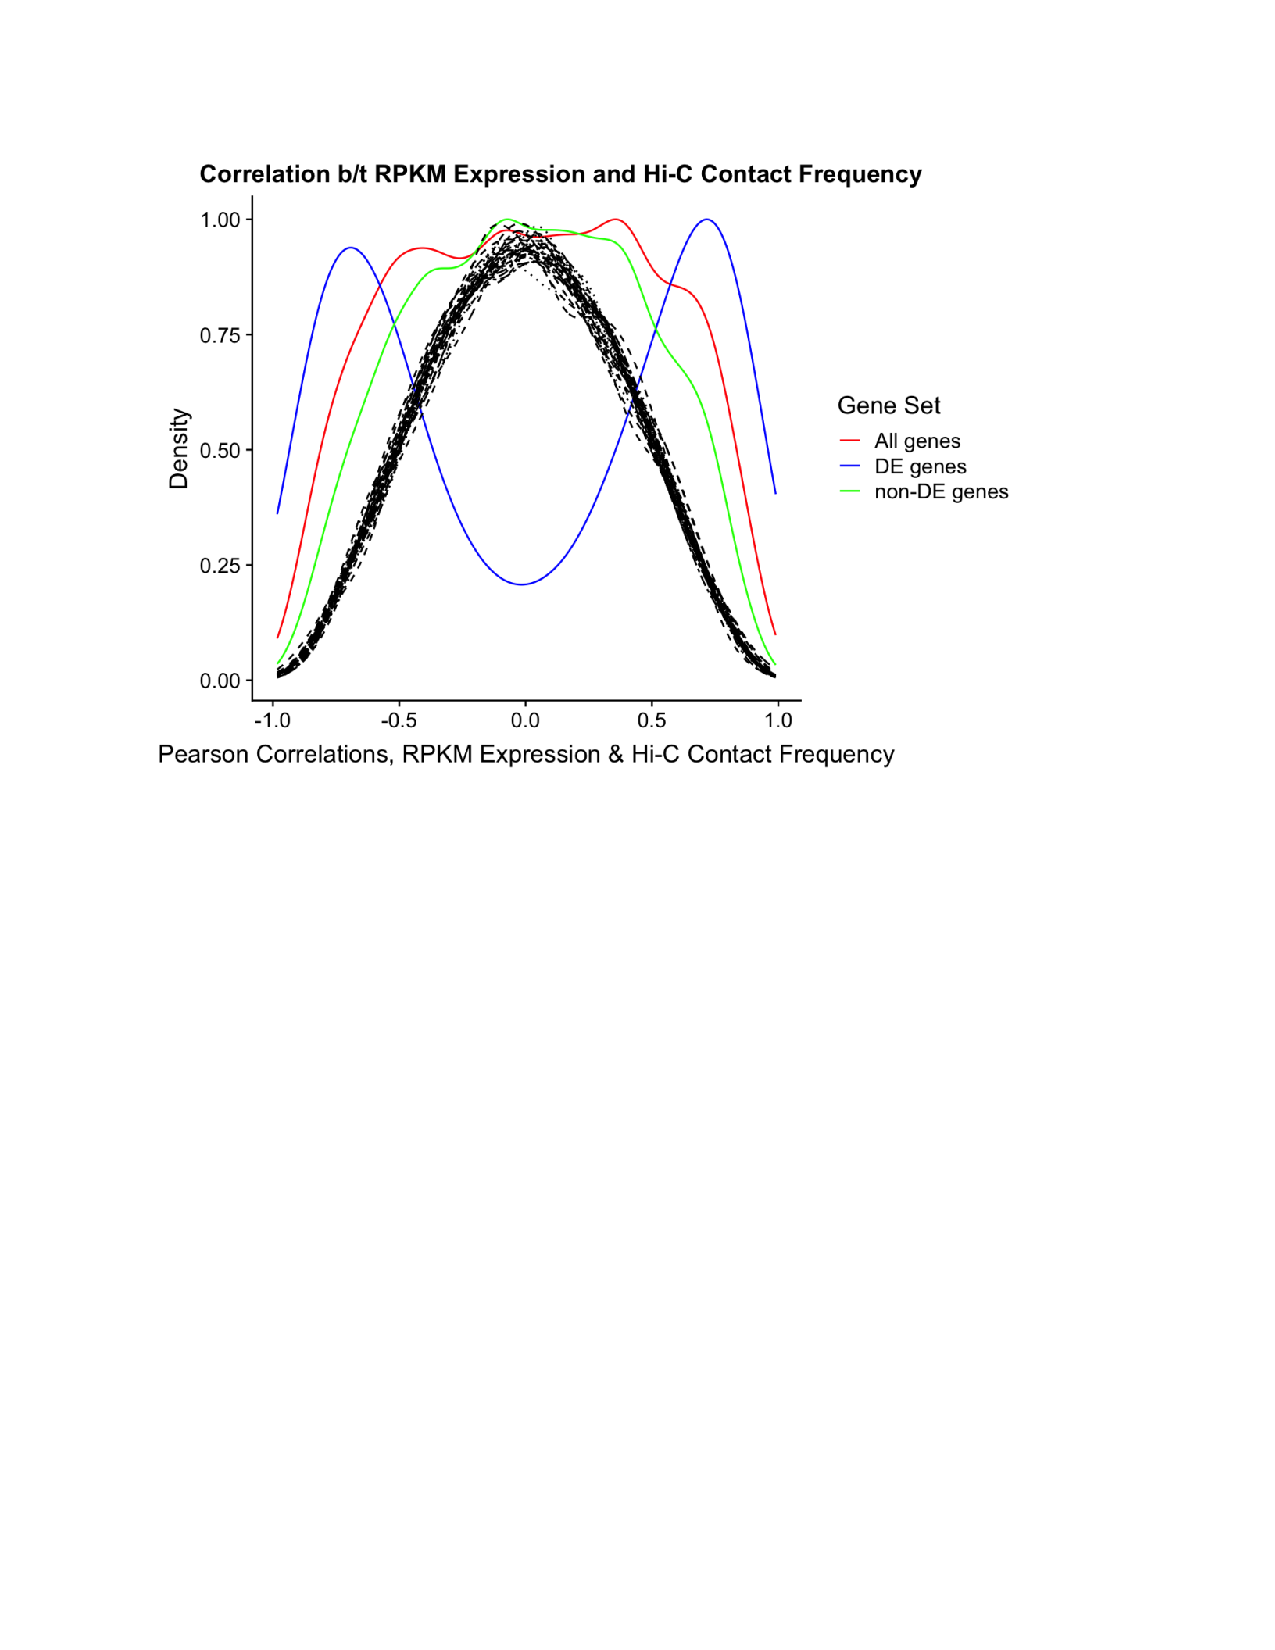
\includegraphics[width=6in]{img/figS15.pdf}
\caption[Correlations between Hi-C and expression.]{\textbf{S15. Correlations between Hi-C and expression.} Density of Pearson correlations between RPKM expression values and log\textsubscript{2} HOMER-normalized contact frequencies across all 8 individuals. Solid lines indicate different sets of the observed data and dotted lines represent 10 permutations of the data. The Hi-C contact frequency chosen is that with the minimum FDR from linear modeling of contact frequency on species (see main text). The strong bimodal distribution of correlations between expression and contact suggests many instances where a contact difference between the species can lead to an increase (enhancer) or decrease (suppressor) of expression in the species where the contact is stronger.}
\label{fig:ch02-figS15}
\end{figure}

\begin{figure}[!htb]
\centering
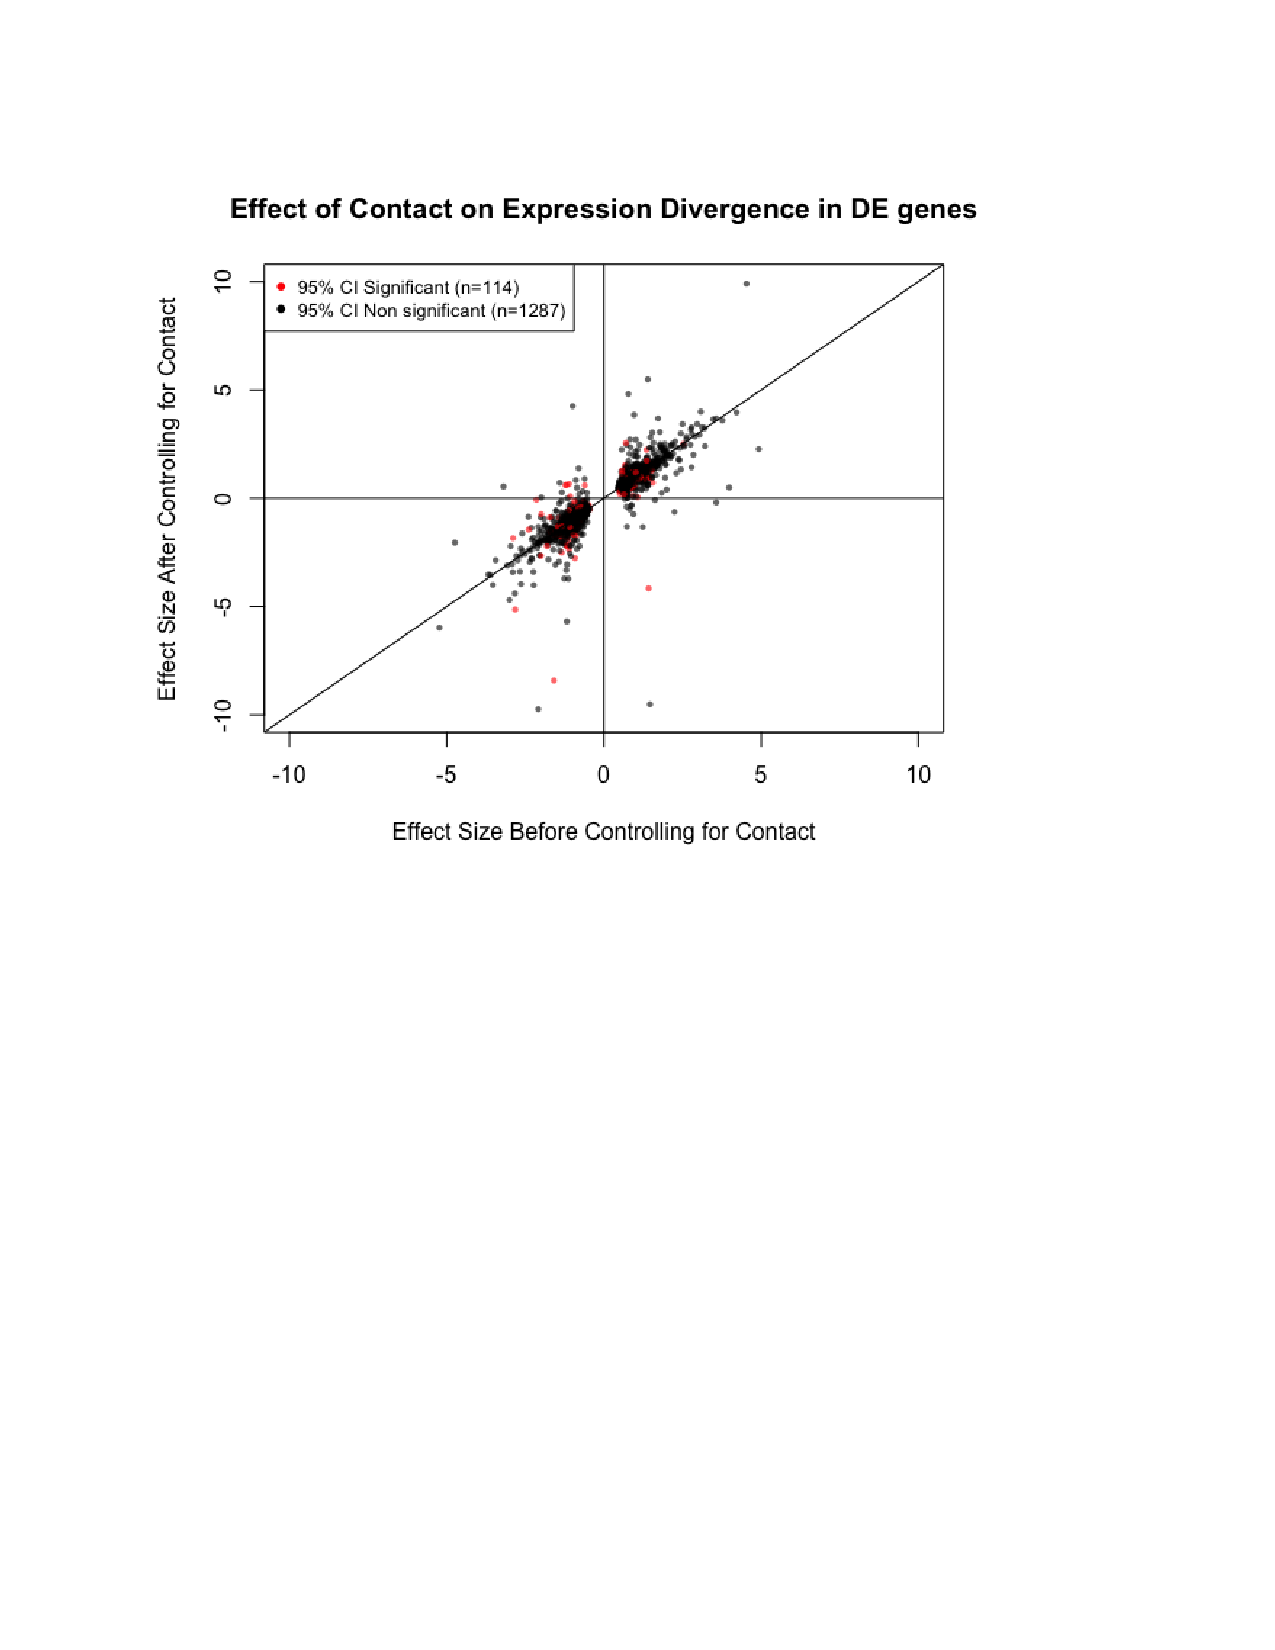
\includegraphics[width=6in]{img/figS16.pdf}
\caption[Gene expression variance is explained by chromatin contacts for 8\% of DE genes.]{\textbf{S16. Gene expression variance is explained by chromatin contacts for 8\% of DE genes.} Plot of the species effect size in DE genes between models before (x-axis) and after (y-axis) conditioning on contact frequency. The Monte Carlo test of significance was used to construct the 95\% confidence interval and evaluate the significance of the indirect effect (species' effect on expression mediated through contact). Amongst DE genes, 8\% (116/1401) of genes showed a statistically significant effect of Hi-C contacts on expression levels (i.e. their 95\% confidence interval does not include zero).}
\label{fig:ch02-figS16}
\end{figure}

\begin{figure}[!htb]
\centering
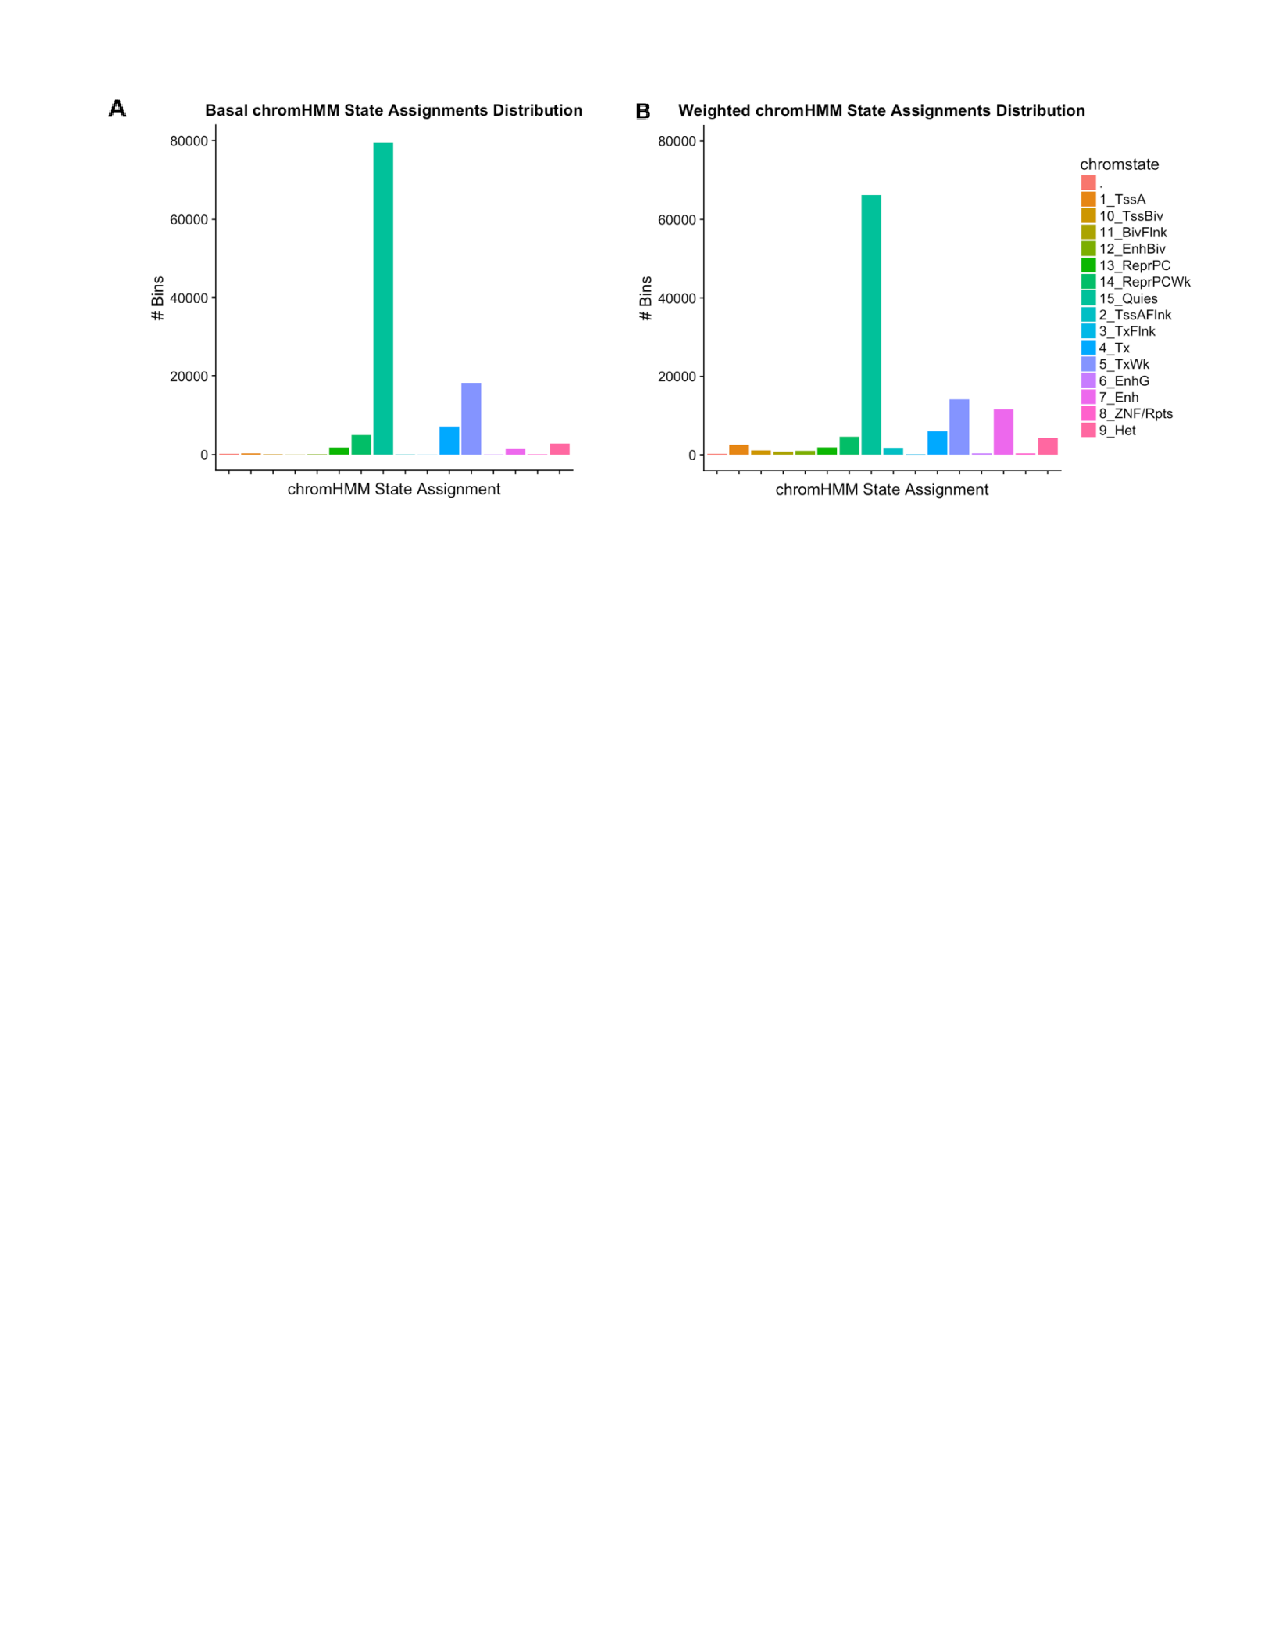
\includegraphics[width=6in]{img/figS17.pdf}
\caption[Using a weighting scheme for chromHMM annotations increases the proportion of transcriptional and enhancer-like annotations.]{\textbf{S17. Using a weighting scheme for chromHMM annotations increases the proportion of transcriptional and enhancer-like annotations.} (A) Histogram showing the number of Hi-C loci (y-axis) assigned to each chromHMM annotation (x-axis) using maximum base pair overlap to assign each locus to a state. In the legend, `.' denotes that no annotation was found for a given bin. (TssA-Active TSS, TSSBiv-Bivalent/Poised TSS, BivFlnk-Flanking Bivalent TSS/Enh, EnhBiv-Bivalent Enhancer, ReprPC-Repressed PolyComb, ReprPCWk-Weak Repressed PolyComb, Quies-Quiescent/Low, TssAFlnk-Flanking Active TSS, TxFlnk-Transcription at gene 5' and 3', Tx-Strong transcription, TxWk-Weak transcription, EnhG-Genic Enhancers, Enh-Enhancers, ZNF/Rpts-ZNF genes and repeats, Het-Heterochromatin). (B) Same as A, only here, we assigned annotations after weighting chromHMM elements' overlaps with Hi-C loci by the reciprocal of their mean overlap in all our loci. This approach increases the number of 10kb Hi-C bins that are assigned to chromHMM annotations associated with transcriptional and enhancer activity (i.e. TssA, TssBiv, TssAFlnk, EnhG, Enh).}
\label{fig:ch02-figS17}
\end{figure}

\begin{figure}[!htb]
\centering
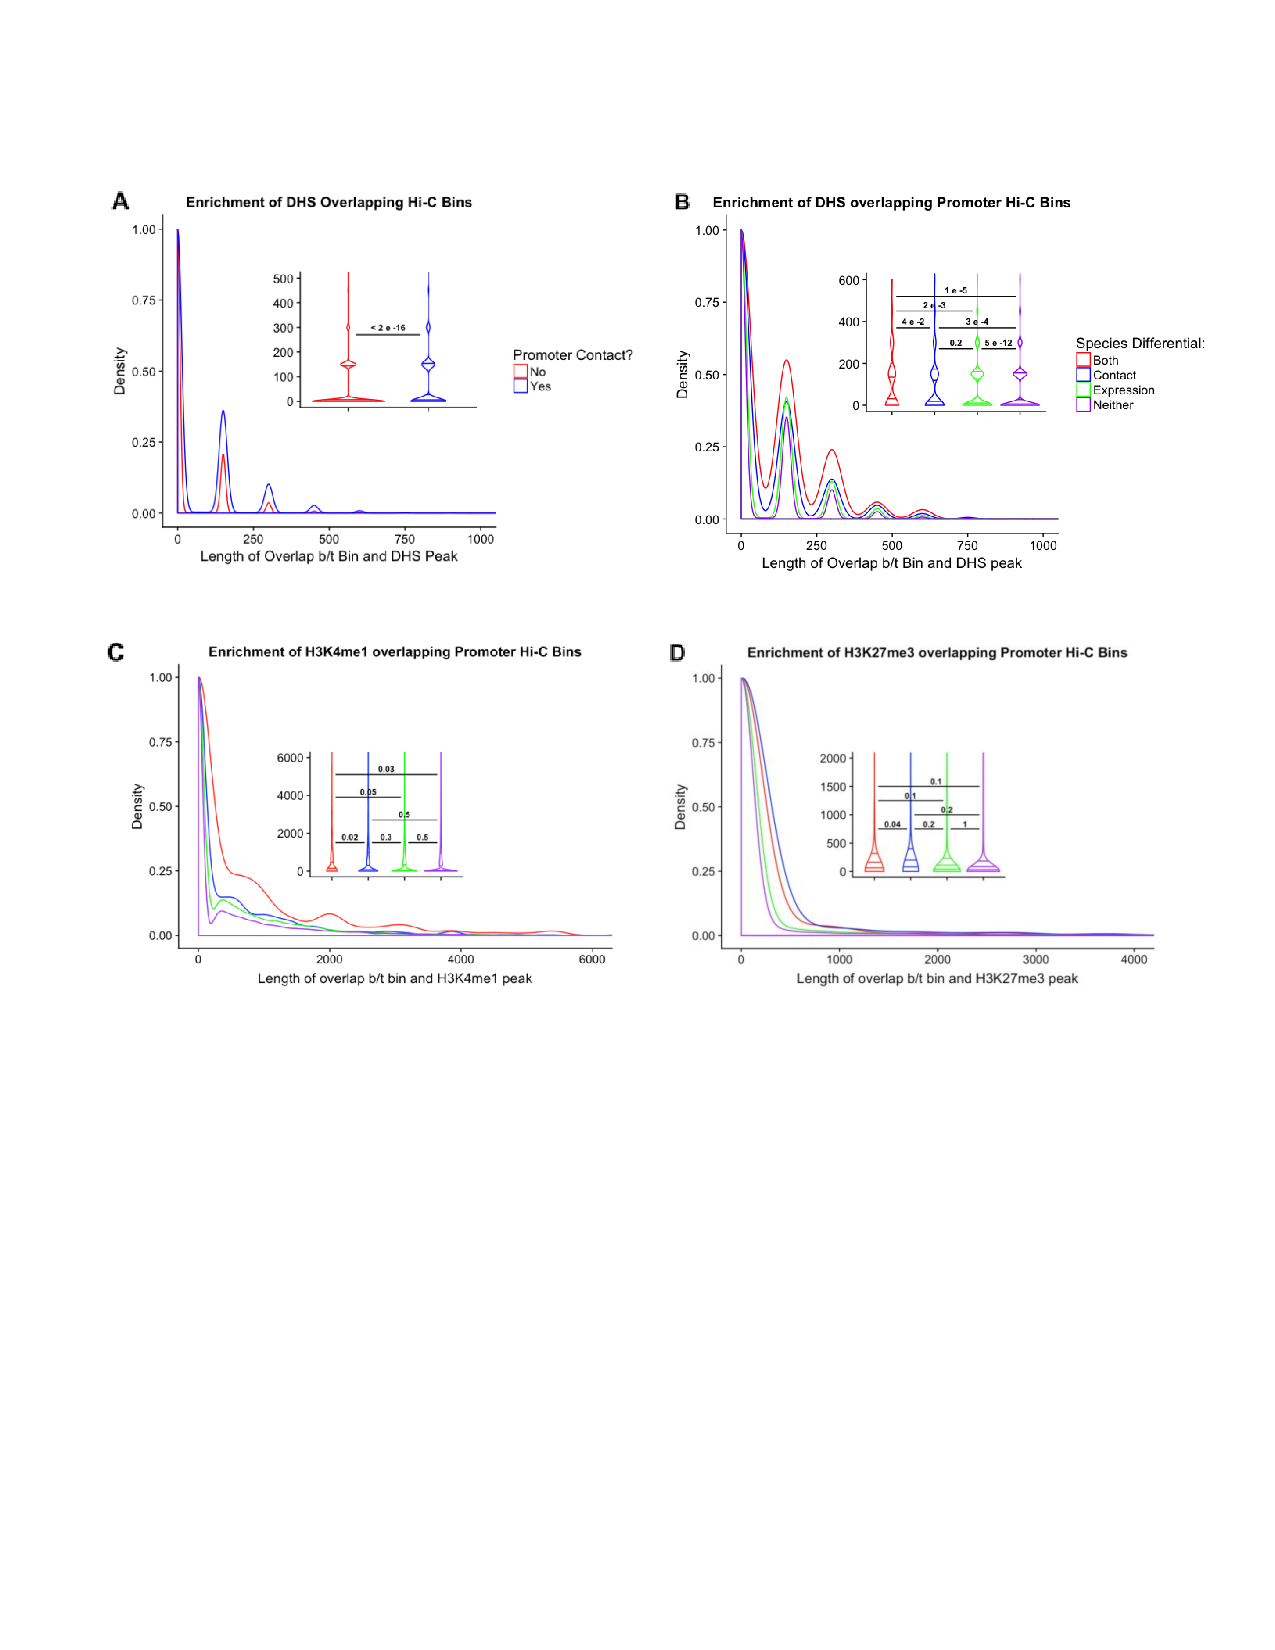
\includegraphics[width=6in]{img/figS18.pdf}
\caption[Overlap of epigenetic signatures and Hi-C contacts.]{\textbf{S18. Overlap of epigenetic signatures and Hi-C contacts.} (A) Density distribution of the base pair overlap between DHS peaks downloaded from ENCODE and our Hi-C loci. Plot is split between Hi-C loci that contact a promoter and those that do not. Inlay is a violin plot of the same distributions, with lines and numbers indicating pairwise t-tests of the mean, and their corresponding significance levels. (B) Density plot similar to A, but only considering Hi-C loci involved in contact with a promoter, and separating contacts into 4 classes, indicated by color: those that show differential contact between species, those that show differential expression between species, those that show both, and those that show neither. We used pairwise t-tests to compare differences in the mean overlap among the four classes of Hi-C loci. (C) Same as in B, but for the active histone mark H3K4me1. (D) Same as in B and C, but for the repressive histone mark H3K27me3.}
\label{fig:ch02-figS18}
\end{figure}

\begin{figure}[!htb]
\centering
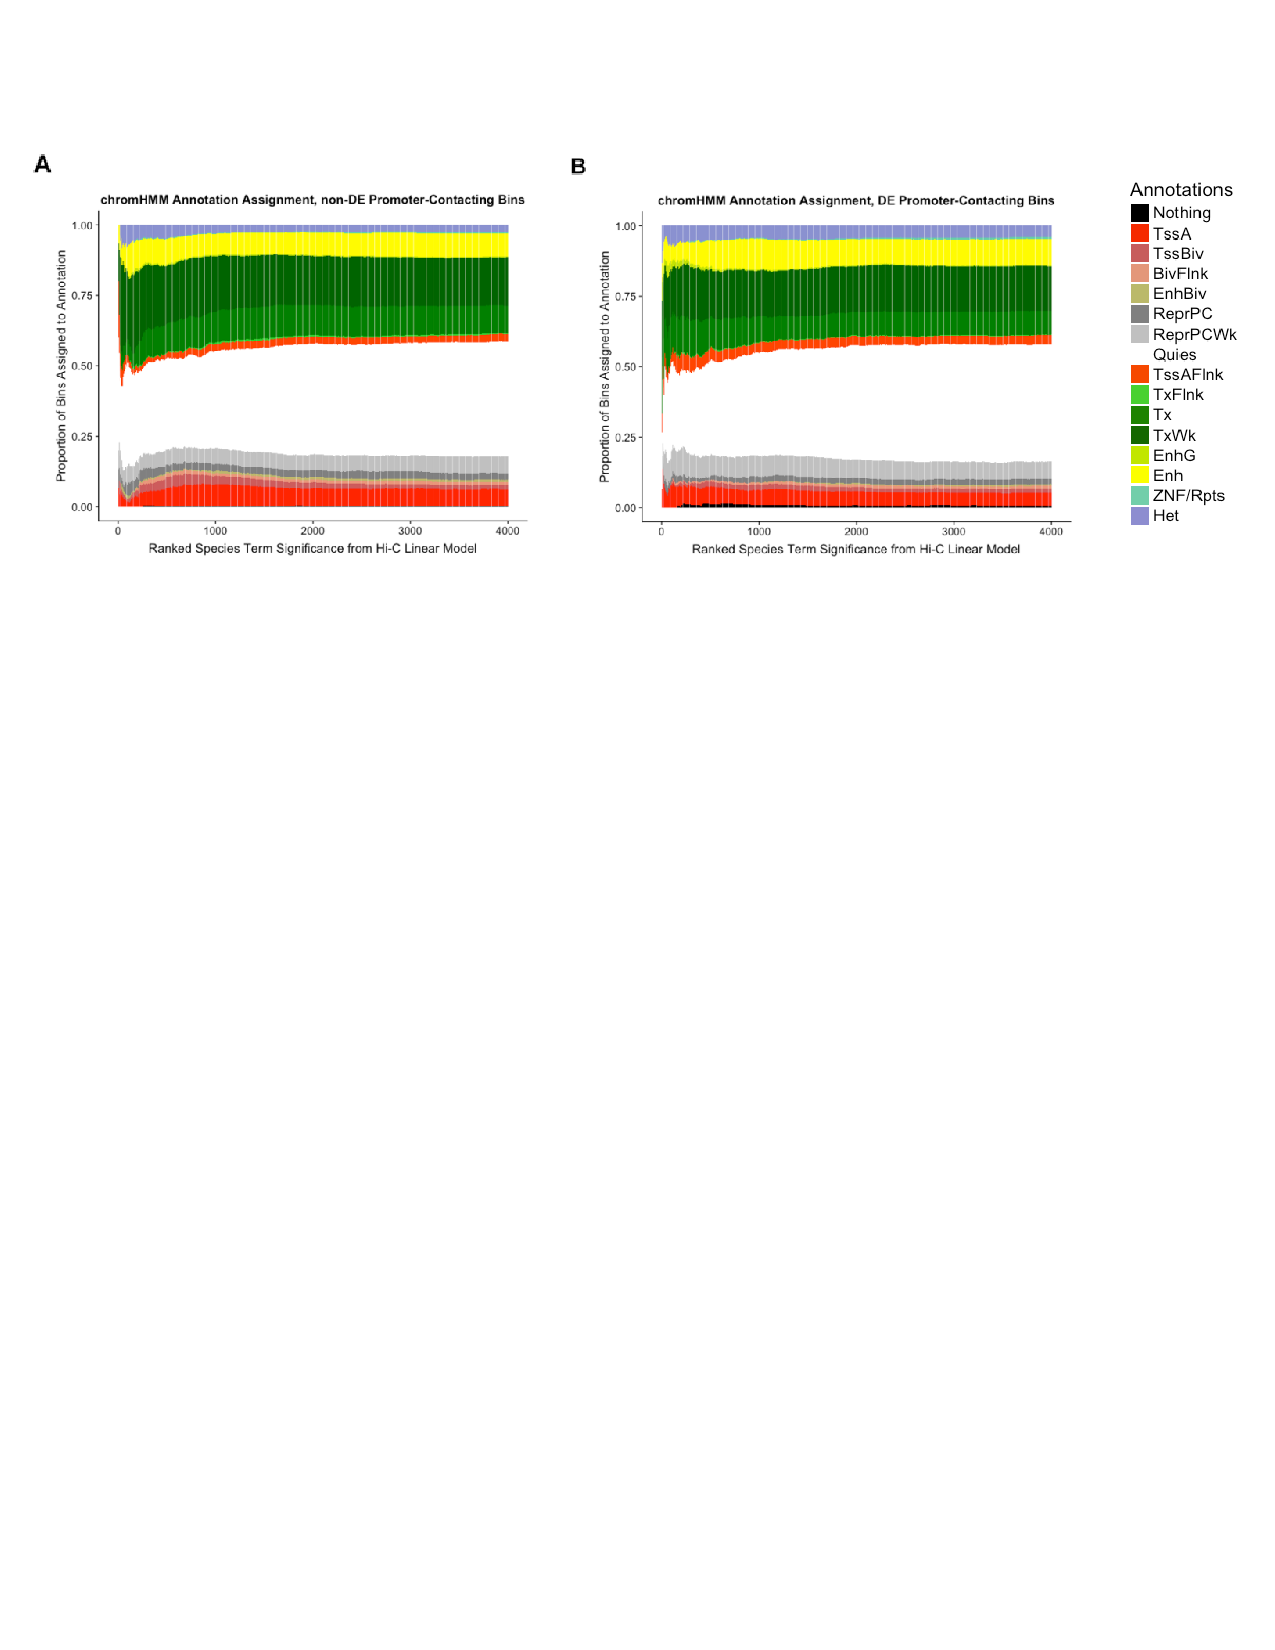
\includegraphics[width=6in]{img/figS19.pdf}
\caption[Dynamics of chromHMM state among significant Hi-C contacts overlapping DE or non-DE genes.]{\textbf{S19. Dynamics of chromHMM state among significant Hi-C contacts overlapping DE or non-DE genes.} (A) Hi-C loci that make contact with promoters of genes that are not differentially expressed (DE) across species are ranked in order of decreasing DC FDR (x-axis). The y-axis shows cumulative proportion of chromHMM annotation assignments for all Hi-C loci at the given FDR or lower. (TssA-Active TSS, TSSBiv-Bivalent/Poised TSS, BivFlnk-Flanking Bivalent TSS/Enh, EnhBiv-Bivalent Enhancer, ReprPC-Repressed PolyComb, ReprPCWk-Weak Repressed PolyComb, Quies-Quiescent/Low, TssAFlnk-Flanking Active TSS, TxFlnk-Transcription at gene 5' and 3', Tx-Strong transcription, TxWk-Weak transcription, EnhG-Genic Enhancers, Enh-Enhancers, ZNF/Rpts-ZNF genes and repeats, Het-Heterochromatin). (B) Same as A, but only considering Hi-C loci making contact with promoters of genes that are differentially expressed (DE).}
\label{fig:ch02-figS19}
\end{figure}

\begin{figure}[!htb]
\centering
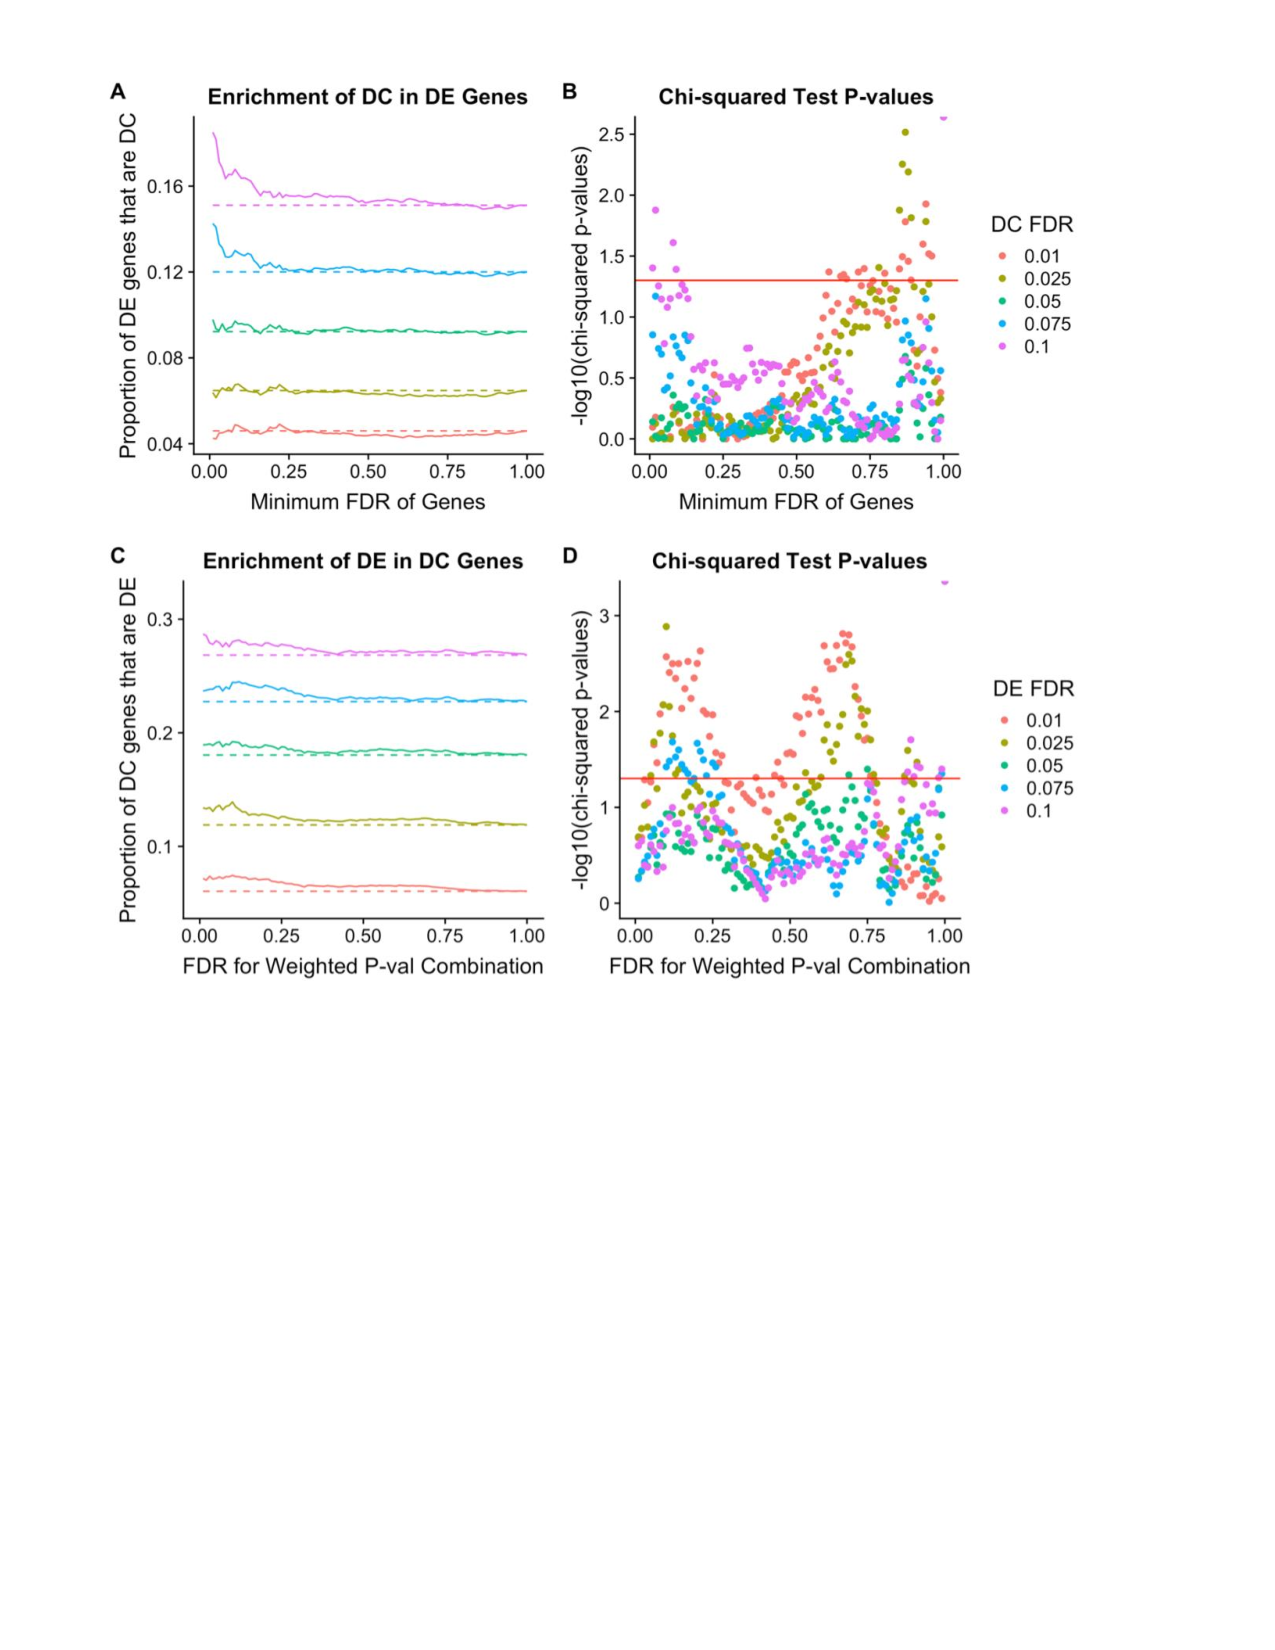
\includegraphics[width=4in]{img/figS20.pdf}
\caption[Reciprocal enrichments of differential expression and differential contact.]{\textbf{S20. Reciprocal enrichments of differential expression and differential contact.} (A) Enrichment of inter-species differentially contacting (DC) loci in genes with corresponding differences in expression (DE) between the species. The proportion of DE genes that are significantly DC (y-axis) is shown across a range of DE FDRs (x-axis). Colors indicate different DC FDR thresholds, and dashed lines indicate the proportion of DC loci expected by chance alone. (B) P values of Chi-squared tests of the null that there is no difference in proportion of DC loci among DE genes (y-axis), shown for a range of DE FDRs (x-axis). In both panels, the DE genes overlapping Hi-C loci were chosen to have the minimum FDR supporting inter-species difference in expression. (C) Similar to Fig 6A, but using a weighted p-value combination technique \cite{Whitlock.2005} to integrate DC FDR across regions, instead of using the minimum FDR DC region. Once again, we observe enrichment of inter-species differentially expressed (DE) genes with corresponding differences in Hi-C contact frequencies (DC) between the species. The proportion of DC genes that are significantly DE (y-axis) is shown across a range of DC FDRs (x-axis). Colors indicate different DE FDR thresholds, and dashed lines indicate the proportion of DE genes expected by chance alone. (D) P values of Chi-squared tests of the null that there is no difference in proportion of DE genes among DC genes (y-axis), shown for a range of DC FDRs (x-axis).}
\label{fig:ch02-figS20}
\end{figure}

\pagebreak
\clearpage

\section{Supplemental Tables}

\begin{table}[!htb]
\caption[S1. HOMER-called contacts, H21792.]{\textbf{S1. HOMER-called contacts, H21792.}}
\label{tab:ch02-s1}
\end{table}

\begin{table}[!htb]
\caption[S2. HOMER-called contacts, H28126.]{\textbf{S2. HOMER-called contacts, H28126.}}
\label{tab:ch02-s2}
\end{table}

\begin{table}[!htb]
\caption[S3. HOMER-called contacts, H28815.]{\textbf{S3. HOMER-called contacts, H28815.}}
\label{tab:ch02-s3}
\end{table}

\begin{table}[!htb]
\caption[S4. HOMER-called contacts, H28834.]{\textbf{S4. HOMER-called contacts, H28834.}}
\label{tab:ch02-s4}
\end{table}

\begin{table}[!htb]
\caption[S5. HOMER-called contacts, C3649.]{\textbf{S5. HOMER-called contacts, C3649.}}
\label{tab:ch02-s5}
\end{table}

\begin{table}[!htb]
\caption[S6. HOMER-called contacts, C40300.]{\textbf{S6. HOMER-called contacts, C40300.}}
\label{tab:ch02-s6}
\end{table}

\begin{table}[!htb]
\caption[S7. HOMER-called contacts, C3624.]{\textbf{S7. HOMER-called contacts, C3624.}}
\label{tab:ch02-s7}
\end{table}

\begin{table}[!htb]
\caption[S8. HOMER-called contacts, C3651.]{\textbf{S8. HOMER-called contacts, C3651.}}
\label{tab:ch02-s8}
\end{table}

\begin{table}[!htb]
\caption[S9. Orthology calling statistics.]{\textbf{S9. Orthology calling statistics.}}
\label{tab:ch02-s9}
\end{table}

\begin{table}[!htb]
\caption[S10. Differentially contacting (DC) regions.]{\textbf{S10. Differentially contacting (DC) regions.}}
\label{tab:ch02-s10}
\end{table}

\begin{table}[!htb]
\caption[S11. Human consensus Arrowhead-inferred TADs.]{\textbf{S11. Human consensus Arrowhead-inferred TADs.}}
\label{tab:ch02-s11}
\end{table}

\begin{table}[!htb]
\caption[S12. Chimpanzee consensus Arrowhead-inferred TADs.]{\textbf{S12. Chimpanzee consensus Arrowhead-inferred TADs.}}
\label{tab:ch02-s12}
\end{table}

\begin{table}[!htb]
\caption[S13. Human-Chimpanzee orthologous TAD coordinates.]{\textbf{S13. Human-Chimpanzee orthologous TAD coordinates.}}
\label{tab:ch02-s13}
\end{table}

\begin{table}[!htb]
\caption[S14. ChromHMM genic enhancer annotation enrichments.]{\textbf{S13. ChromHMM genic enhancer annotation enrichments.}}
\label{tab:ch02-s14}
\end{table}

\begin{table}[!htb]
\caption[S15. ENCODE chromatin mark sources.]{\textbf{S15. ENCODE chromatin mark sources.}}
\label{tab:ch02-s15}
\end{table}

\begin{table}[!htb]
\caption[S16. Sample metadata.]{\textbf{S16. Sample metadata.}}
\label{tab:ch02-s16}
\end{table}

\begin{table}[!htb]
\caption[S17. 10kb Arrowhead TAD inferences, H21792.]{\textbf{S17. 10kb Arrowhead TAD inferences, H21792.}}
\label{tab:ch02-s17}
\end{table}

\begin{table}[!htb]
\caption[S18. 10kb Arrowhead TAD inferences, H28126.]{\textbf{S18. 10kb Arrowhead TAD inferences, H28126.}}
\label{tab:ch02-s18}
\end{table}

\begin{table}[!htb]
\caption[S19. 10kb Arrowhead TAD inferences, H28815.]{\textbf{S19. 10kb Arrowhead TAD inferences, H28815.}}
\label{tab:ch02-s19}
\end{table}

\begin{table}[!htb]
\caption[S20. 10kb Arrowhead TAD inferences, H28834.]{\textbf{S20. 10kb Arrowhead TAD inferences, H28834.}}
\label{tab:ch02-s20}
\end{table}

\begin{table}[!htb]
\caption[S21. 10kb Arrowhead TAD inferences, C3649.]{\textbf{S21. 10kb Arrowhead TAD inferences, C3649.}}
\label{tab:ch02-s21}
\end{table}

\begin{table}[!htb]
\caption[S22. 10kb Arrowhead TAD inferences, C40300.]{\textbf{S22. 10kb Arrowhead TAD inferences, C40300.}}
\label{tab:ch02-s22}
\end{table}

\begin{table}[!htb]
\caption[S23. 10kb Arrowhead TAD inferences, C3624.]{\textbf{S23. 10kb Arrowhead TAD inferences, C3624.}}
\label{tab:ch02-s23}
\end{table}

\begin{table}[!htb]
\caption[S24. 10kb Arrowhead TAD inferences, C3651.]{\textbf{S24. 10kb Arrowhead TAD inferences, C3651.}}
\label{tab:ch02-s24}
\end{table}



% Chapter 03 - Review Paper
\chapter{A TAD Skeptic: Is 3D Genome Topology Evolutionarily Conserved?}\label{ch:ch03}

\section[Abstract]{Abstract\footnotemark}

The notion that topologically associating domains (TADs) are highly conserved across species has practically become an axiom in the field of 3D genome research. But what exactly do we mean by `highly conserved', and what are the actual comparative data that support this notion? To address these questions, we performed a historical review of the relevant literature, and retraced numerous citation chains to reveal the primary data that were used as the basis for the widely accepted conclusion that TADs are highly conserved across evolution. A thorough review of the available evidence suggests the answer may be more complex than what is commonly presented.

\footnotetext{Citation for chapter: Eres, Ittai E, and Gilad, Y. A TAD Skeptic: Is 3D Genome Topology Evolutionarily Conserved? \textit{Manuscript in review at Trends in Genetics}}

\section{What are TADs?}
Some of the most fascinating features to have emerged from research into 3D genome conformation are topologically associating domains (TADs). Originally discovered through the analysis of Hi-C data \cite{Dixon.2012, Nora.2012, Hou.2012, Sexton.2012}, TADs appear on a chromatin contact map as large squares of enhanced contact frequency rising off the diagonal. The original method for algorithmic TAD inference used a `directionality index' \cite{Dixon.2012} to define TADs as segments of the genome that are more connected to each other than to other regions.  In turn, TAD boundaries were defined as segments of the genome that are characterized by a sharp transition between upstream and downstream highly connected regions. Originally applying directionality index to Hi-C data at the relative low resolution of 40 kb, early studies reported that TADs are non-overlapping, highly self-interacting megabase-scale structures. More recent studies, using higher-resolution contact maps, as well as different inference algorithms, have revealed TAD structures at much smaller scales, and often nested within each other \cite{Phillips-Cremins.2013, Berlivet.2013, Rao.2014}. The precise nature of these features is still a matter of debate, with various definitions of TADs shifting as new algorithms arise and new discoveries are made about the mechanisms behind TAD formation (e.g. loop extrusion and compartmentalization) \cite{Phillips-Cremins.2013, Rao.2014, Filippova.2014, Dixon.2016, Zhan.2017, Nuebler.2018, Fudenberg.2016, Sanborn.2015}. Previous studies have found relatively low concordance of TADs defined by different algorithms and across various resolutions and parameters, further impeding a robust definition of these structures \cite{Dali.2017, Forcato.2017, Zufferey.2018}. While efforts have been made to functionally delineate between TADs at different scales \cite{Dixon.2016, Beagan.2020, Sikorska.2019, Szabo.2019}, most studies, especially those who rely solely on Hi-C data, do not make these distinctions.

Regardless of the challenge of defining TADs, it is clear that these 3D structures play an important role in genome organization and function \cite{Berlivet.2013, Dixon.2016, Beagan.2020, Andrey.2017, Franke.2018, Xie.2019, Dixon.2015, Delaneau.2019, Smith.2016}. Studies assessing the direct transcriptional effects of TADs have found mixed results, with some locus-specific work suggesting a strong impact of TAD disruption on gene expression \cite{Lupianez.2015, Hnisz.2016, Guo.2015, Laugsch.2019}, while other genome-wide results imply only mild effects on expression \cite{Ghavi-Helm.2019, Zuin.2014, Espinola.2020, Rao.2017}. Despite some uncertainty about the magnitude of regulatory changes induced by TAD disruptions, multiple independent lines of evidence suggest TADs are functionally relevant. Genes located within the same TAD can have strongly correlated expression patterns and are often coregulated during cell differentiation \cite{Nora.2012, Zhan.2017, Ramirez.2018}. TAD boundaries are strongly correlated with replication-timing domain boundaries \cite{Pope.2014}, and are enriched for insulator elements such as CCCTC-binding factor (CTCF) \cite{Dixon.2012, Rao.2014}. Disruptions in normative TAD structures have also been implicated in a number of human pathologies \cite{Lupianez.2016, Ibn-Salem.2014, Franke.2016}. While precise and robust TAD and boundaries definitions are still elusive, a general feature that is robust to the specific definition is that loci within a TAD make contact more frequently with other loci in the same TAD than with loci outside it. The common paradigm is that TADs represent insulated neighborhoods, constraining the possible set of interactions between cis regulatory elements (CREs) and target genes \cite{Andrey.2017, Franke.2018, Dixon.2015, Delaneau.2019, Smith.2016, Symmons.2014, Tanay.2013}. It is believed that TADs are critical features of the genome, serving to sustain specific sets of regulatory interactions while preventing ectopic interactions between regulatory elements and the wrong target genes \cite{Andrey.2017, Symmons.2014, Sexton.2015}.

Numerous other papers and reviews have delved into the history and functionality of TADs. Previous papers and reviews discuss the variance in algorithmic identification of TADs, the inconsistency of TAD calls at different resolutions, and the lack of robust approach to identify TAD boundaries based on Hi- C data \cite{Dixon.2016, Beagan.2020, Dali.2017, Forcato.2017, Zufferey.2018, Sikorska.2019, Andrey.2017, Franke.2018, Schoenfelder.2019, Rowley.2018, Fraser.2015, Ay.2015}. The notion that TADs are highly conserved across species and cell types is prevalent and often considered a foregone conclusion. Determining TAD variability across cell types is important for understanding the extent to which 3D genome structure affects differential gene regulation during development, enabling the regulatory and functional novelty observed in different cell lineages. In turn, assessing TAD conservation across evolution could help reveal the regulatory loci and mechanisms responsible for speciation and adaptation. We do not discuss further the issues related to similarities and differences in TADs across cell types and tissues, which have been previously discussed \cite{Andrey.2017, Sauerwald.2018, Sauerwald.2019, Schmitt.2016, Zheng.2019, Bonev.2016, Cubenas-potts.2015}. In this review, we wish to specifically focus on the notion that TADs and their boundaries are highly conserved across species.

Many studies are cited as reporting this conclusion, but it is difficult to trace the origin of this claim. If TADs and their boundaries are indeed highly conserved across spices, the origin of regulatory novelty must be elsewhere. However, if genome organization is not highly conserved, it is possible that changes in TADs and insulation boundaries may play an important role in underlying adaptation and speciation through changes in gene regulation. In other words, the answer to the question of TAD conservation has important implications for evolutionary research. We thus set out to thoroughly review the evidence for TAD conservation and we found that, in fact, only a few studies collected relevant data and provide direct evidence to support this notion.

\section{Conservation in Context}
In order to evaluate the evidence for conservation of TADs, it is important to consider what we actually mean when we refer to conservation of genetic and epigenetic features across species. At the level of a single feature{\textemdash}a single locus for example{\textemdash}conservation is easily defined when the state of the feature is identical across species. More generally, however, when studies refer to genome-wide properties, they typically do not use a specific standard for the definition of conservation. When studies refer to a general property (for example, chromatin accessibility) as conserved, it implies that this property evolves under natural selection to maintain similarity across species. However, very few studies formally test this hypothesis. In fact, for most functional genomic traits that are comparatively studied, we have not yet formulated as null model of `no selection.' 
Without a formal test, what do we typically mean when we conclude that a molecular trait is conserved? In most studies, conservation simply means `highly similar' across species. While this is typically not a formal process, the degree of similarity, or variance, is evaluated and benchmarked based on other relevant comparisons. For example, if the level of observed variation in a trait is similar within and between species, the trait is typically deemed highly similar across species and therefore conserved. If variation between species is consistently low regardless of the time to the most recent common ancestors of the species, the trait is likely to be conserved. If different molecular features show a range of inter-species variability, the features with the lowest variance across species are assumed to be conserved. All of these examples point to ad-hoc definition of conservation, but this does not mean that they are wrong.

Let us consider specific examples. Comparative studies have reported that genome-wide, the overlap of histone modification H3K4me3 locations in humans and chimpanzees is around 70\% \cite{Cain.2011}. Remarkably, the genome-wide overlap of H3K4me3 locations in humans and mouse is also around 70\% \cite{Woo.2012}. With these figures, not much could be said about the conservation of H3K4me3 locations in primates, but we can probably conclude with confidence that H3K4me3 locations are quite conserved between human and mouse. That said, the best genomic context for evaluating the degree of conservation in these comparisons may be other histone modifications, but even the minimal context provided here illustrates the importance of benchmarking similarity values in order to understand what they imply about conservation across species. 

To date, comparative studies of chromatin conformations and TADs did not put forward a formal null model with which to evaluate levels of conservation. Instead, statements regarding the conservation of TAD and boundaries were made by using the ad-hoc rationale we discussed above. With this in mind, we now turn to critically examine the existing evidence for evolutionary conservation of TADs.

\section{Indirect evidence for conservation}
The notion that TADs and are highly conserved appears to be supported by a number of studies. One class of such studies, however, does not perform direct comparative assessment of TADs and boundaries across species. Instead, the indirect inference of TAD conservation is based on comparative functional genomic data that are independently associated with TADs. The most common approach in this class of studies is to directly map TADs in one species, then infer the locations of TADs in other species based on genomic features that are associated with TADs, such as CTCF binding sites, high gene density, or regions of active transcription \cite{Dixon.2012, Nora.2012, Rudan.2015, Kentepozidou.2020, Dekker.2015}. To date, however, no single genomic feature can be used to effectively predict TAD locations and boundaries. Thus, the inference of TAD conservation based on other functional genomic features is indirect and might not be accurate. 

One of the most commonly cited studies supporting TAD conservation, Rudan et al. 2015 \cite{Rudan.2015}, used such an indirect inference approach. Rudan et al. 2015 \cite{Rudan.2015} collected comparative Hi-C data in liver cells from mouse, macaque, rabbit, and dog, but most of their comparative inference was based on the placement and orientation of CTCF binding sites. The authors conclusion that there is ``extensive genome-wide interspecies conservation of chromosome structure'' was based on comparisons of a broader set of contacts, not specifically of TADs. In fact, Rudan et al. did not report the total number of TADs identified in each species (only in mouse and dog), nor did they directly estimate the proportion of TADs that are found to be conserved across species. Instead, they used an indirect measure, estimating the interspecies correlations of inferred insulator activity \cite{Sofueva.2013} at different distances from orthologous genes. Rudan et al only reported species pairwise comparisons that involved the mouse data, resulting in Spearman correlations that ranged from 0.34 to 0.61. These correlations values may indicate some degree of conservation of 3D genome structure, but it is difficult to conclude from these analyses that TADs are indeed highly conserved across species. Moreover, Rudan et al. data collection was uneven across species, with ~275 million reads sequenced from mouse, ~150 million from rabbit, ~100 million from macaque, and ~550 million for dog. The large differences in read count result in a difference in the power to identify 3D genome structures across species and hence complicate the interpretation of the reported results. 

There are other widely cited studies that concluded that TADs are highly conserved based on indirect evidence. Harmston et al. 2017 \cite{Harmston.2017}, for instance, identified genomic regulatory blocks (GRBs, regions with a high density of conserved noncoding elements) in human, opossum, chicken, and spotted gar. They reported that GRBs are often quite conserved across species. Using previously collected Hi-C data from human and Drosophila, Harmston et al. have shown that GRBs often fall within TADs and/or have edges proximal to TAD boundaries in these two species. Based on these data, the authors concluded that TADs are generally conserved ancient features of the genome and that TAD boundaries are largely invariant between all  the species in their study. However, the data reported by Harmston et al. shows that only about a third of the TADs were associated with GRBs; thus, even if one accepts the indirect inference based on GRBs as correct, up two thirds of TADs may still not be conserved in these species, as no direct evidence for TAD conservation was presented in this study. Indeed, in their concluding statement, Harmston et al. are careful to note that only the subset of GRB-associated TADs appears to be ancient conserved structures. However, this paper is often cited as providing strong evidence for general TAD conservation across species.  

Similarly, Krefting et al. 2018 \cite{Krefting.2018} considered TADs that were previously directly identified in humans \cite{Dixon.2012, Rao.2014} along with genomic rearrangement breakpoints they identified in 13 species. Based on observed enrichment of these breakpoints at TAD boundaries and depletion within TAD bodies, the authors made relatively strong claims about TAD stability across evolutionary timescales. However, no direct comparison of TADs was made across species; the conclusions are essentially only based on the inter-species comparison of the rearrangement breakpoints. Given this, that the enrichments observed were only in comparison to TADs found in humans, and a fair amount of inconsistency in the degree of enrichment observed between the two different TAD sets used, we do not believe strong claims of conservation are warranted. Motivated by the findings of Harmston et al. 2017 \cite{Harmston.2017}, the same study also examined correlation of gene expression for orthologous genes in humans and mice within TADs associated with GRBs vs. orthologous genes in non-GRB associated TADs. While they found that gene expression within GRB-associated TADs is significantly slightly more correlated than the expression of non-GRB TAD genes, they also noted that more than 60\% of hESC TADs don't overlap GRBs, perhaps suggesting that only a small subset of TADs are actually conserved. The authors should be commended for making note of this, as well as including the caveat that the enrichment they observe may be due to chromatin accessibility differences between TAD boundaries and TAD bodies. Still, the majority of the paper makes claims of TAD conservation across evolutionary timescales, which simply are not supported due to inconsistent enrichments across different TAD sets and a lack of TAD inferences in any species aside from humans.

In another comparable approach, Lazar et al. 2018 \cite{Lazar.2018} chose to compare human and gibbon genomes in LCLs, given the large number of chromosomal rearrangements and high DNA sequence identity (96\%) between the two species. The authors cite previous studies to substantiate the claim that TADs are largely conserved across species \cite{Dixon.2012, Rudan.2015}, and ultimately conclude that most TADs have been maintained as `intact modules' during genomic divergence between humans and gibbons. Such claims may be overstated, given that this work did not undertake a direct comparison of TAD locations between the species, instead largely focusing on the overlap of multiple species\' TAD boundaries with 67 rearrangement breakpoints identified in the gibbon genome (in comparison to human). Though their results indicate a high overlap of TAD boundaries across multiple species with gibbon breakpoints above what would be expected at random, they do not, to us, indicate strong conservation of the TADs themselves across species. Our interpretation is further supported by the study\'s finding that only 19 of the 67 breakpoints (~28\%) overlapped TAD boundaries in all other species compared (human, rhesus, mouse, dog, and rabbit). Conversely, the authors found almost no evidence for new TADs being created between humans and gibbons based on rearrangement breakpoints, but we note again that this analysis is focused on the breakpoints rather than the TADs, and that the absence of evidence does not indicate evidence of absence.

Finally, we wish to highlight one exemplary study that also did not perform a direct assessment of TADs across species, but was measured in its conclusions and made a significant methodological contribution to comparative analysis of 3D genome topology. Yang et al. 2019 \cite{Yang.2019} represents one of the only papers with an explicit aim of comparing 3D genome organization across a number of primate species, and sequenced a similar number of Hi-C reads from LCLs in chimpanzees, bonobos, and gorillas, in addition to examining previously-published human Hi-C data in the same cell type \cite{Rao.2014}. The analysis framework they present for interspecies comparison\emdash phylo-HMRF (hidden markov random field)\emdash is sorely needed for interspecies comparative Hi-C.  The robustness of the method is also underscored by the proximity between its identified boundaries of Hi-C evolutionary pattern blocks and previously-inferred TAD boundaries \cite{Rao.2014}. We speculate that the authors focused on this overlap, rather than directly inferring TADs in the novel primate Hi-C datasets collected, because direct TAD inference and comparison would not be robust, just as general TAD inference is not robust. Despite similar sequencing depth across species, TAD detection would likely be confounded by differences in reference genome quality, a consideration the authors apparently took quite seriously, given that all Hi-C reads in the method are ultimately mapped back to the human reference genome. To our knowledge, this is one of the only papers presenting an analytical framework for interspecies Hi-C comparison, with the other being more focused on similarity of genomic contacts within orthologous TADs between species, rather than the locations of the TADs  \cite{Nuriddinov.2019}. As both of these methods are relatively recent,  they have not yet been more broadly applied to a wide range of Hi-C datasets across different species, but we look forward to such analyses being used in the future in our own work and that of others.

In summary, all of the studies we discussed in this section did not directly identify TADs in multiple species, could not perform a direct inter-species comparison of TADs, and thus these studies do not provide direct evidence for the notion that TADs are highly conserved. In order to truly understand the extent of conservation of these structures, we must infer and examine them across a number of species, and assess if a given TAD in one species has a corresponding counterpart in others. Otherwise, claims of conservation speak to conservation of features of TADs and 3D genome topology more broadly, rather than conservation of the individual structures themselves.

\section{Direct but anecdotal evidence for conservation}
The second class of studies that are widely cited as providing evidence for general TAD conservation provide only anecdotal evidence. These are studies that provide direct and strong evidence for conservation of TADs, but only in a small number of well-studied cases. It is thus difficult to generalize from these studies and conclude with confidence that TADs are generally highly conserved across species.

Woltering et al. 2014 \cite{Woltering.2014}, for example, found that Hox loci across zebrafish and mouse tend to have similar TAD structure, and Gomez-Marin et al. 2015 found comparable TAD structures across a number of species at the Six loci \cite{Gomez-marin.2015}. Both of these studies, as well as a number of others \cite{Smith.2016, Lupianez.2015, Galupa.2018, Galupa.2020}, focus on loci that are highly conserved and/or thought to be critical for normal organismal development. Though these findings underscore the functional importance of TADs, they do not provide evidence for broad and general TAD conservation. In particular, the focus on a subset of candidate loci that are more likely to contain conserved features makes it difficult to generalize these observations to a genome-wide scale. Thus, though these studies infer TAD conservation based on direct functional data, they do not provide strong support for the widely accepted notion that TADs are highly conserved. 

\section{Direct evidence for the conservation of TADs}
We now turn to the relatively small body of research that studied TAD conservation by directly identifying TADs and boundaries in multiple species. This direct approach seems the most obvious. In fact, it would be challenging to find another example in the genomics field where a widely accepted conclusion was mostly supported by indirect evidence and inference. In the case of comparative studies of TADs, only a few studies collected direct comparative data.

Dixon et al. 2012 \cite{Dixon.2012} collected Hi-C data and inferred TADs in human and mouse. This study was groundbreaking as it was one of the first to discover TADs and propose an algorithm to infer them from Hi-C contact maps (directionality index). This study is often cited as providing the first evidence that TADs are highly conserved between humans and mice. The authors collected 475 million sequencing reads from mouse Hi-C libraries but only 330 million reads from human. TAD boundaries were considered conserved if they had any overlap in the other species, with 76\% of mouse TAD boundaries found in humans but only 54\% of human boundaries found in mice. If one considers the entire dataset of TAD boundaries identified in both human and mouse (rather than the reported unilateral overlaps), ~31\% of boundaries are shared across the two species.

These results were and still are interpreted as evidence for strong TAD conservation. To provide some context, we considered other functional annotations in human and mouse. There is about 60-75\% overlap of loci marked by histone modification in humans and mice \cite{Woo.2012}, and between half to two-thirds of candidate regulatory regions are conserved in the two species \cite{Yue.2014}. Considering the observed proportion of overlapping TAD boundaries in human and mouse in this context, we believe that there is evidence for some level of conservation, but arguably, this cannot be considered strong evidence that TADs are generally highly conserved across species.

Another study that performed a direct comparative assessment of TADs is Rao et al. 2014 \cite{Rao.2014}. The authors collected ~6.5 billion Hi-C sequencing reads from human but only ~1.4 billion reads from mouse. The difference in read depth resulted in a striking difference in the power to infer TADs in the two species, with more than 9000 domains identified in human but only ~3000 domains found in mouse. The authors considered entire domains conserved if the center of a domain in one species was within 50 kb of an annotated domain in the other species (or within half the domain size, for domains smaller than 100 kb). Ultimately, Rao et al. 2014 reported that 45\% of mouse domains (where they had considerably less power to identify TADs) were also present in human. Again, there may be some evidence for conservation, but it is difficult to conclude based on these data that TADs are highly conserved. 

As far as we know, Dixon et al. 2012 and Rao et al. 2014 are two of the only studies that concluded that TADs are highly conserved based on a direct analysis of TADs and boundaries in more than one species. Both works used human and mouse, and utilized an unbalanced sequencing study design across species, which makes the interpretation of the results somewhat challenging. Regardless, even if we accept the observation of Dixon et al. 2012 and Rao et al. 2014 at face value, the reported overlap of TADs and boundaries in human and mouse arguably does not indicate that these features are highly conserved.

\section{On the other hand...}
There are a few studies that suggest that TADs may not be particularly conserved across species. Berthelot et al. 2015 \cite{Berthelot.2015} considered the order of orthologous genes to identify genomic rearrangement breakpoints in the genomes of human, mouse, dog, cow, horse, and a genomic reconstruction of the Boreoeutherian last common ancestor. In an attempt to understand the non-random genomic distribution of these breakpoints, the authors considered the overlap of rearrangement breakpoints with TADs that were previously identified in human \cite{Dixon.2012}. Because the basal set used for comparisons was breakpoints rather than TAD boundaries, this is another example of a study that relied on indirect inference. In contrast to the results described from Lazar et al. \cite{Lazar.2018}, the authors did not find evidence for strong overlap of TAD boundaries and breakpoints, reporting that only 8\% of the identified breakpoints overlap with TAD boundaries. This would suggest that TADs do not generally contribute to the locations of genomic rearrangements.

Berthelot et al. 2015 \cite{Berthelot.2015} is also notable for its interpretation of the results of Dixon et al. 2012 \cite{Dixon.2012}. While the vast majority of papers cite Dixon et al.\'s study as providing strong evidence that TADs are highly conserved, Berthelot et al. cite the same study to provide evidence for some TAD divergence between humans and mice. That the results of Dixon et al. 2012 can be interpreted by different groups both as supporting conservation of TADs or lack thereof highlights our notion that the foundation for the claim that TADs are highly conserved is not strong.

The notion that TADs may not be particularly conserved is also supported by our own study, in which we directly inferred TADs in humans and chimpanzees \cite{Eres.2019}. Our initial analysis found only ~43\% of TADs conserved between these species, but across many different parameters (e.g. resolution, window size, genome assembly), and different downstream analysis decisions, we found that no more than 78\% of domains and 83\% of TAD boundaries were shared between humans and chimpanzees{\textemdash}a much lower percentage than what has been seen across these species for a number of other functional regulatory phenotypes.

The notion that TADs may not be particularly conserved is also supported by recent results from Hi-C data across three distantly related Drosophila species. Renschler et al. 2019 \cite{Renschler.2019} inferred TADs and genomic rearrangements across three Drosophila species, and found significant overlap above what would be expected by chance alone. However, the percentages of TAD boundaries overlapping a rearrangement breakpoint were relatively low (ranging from 13-21\% of boundaries depending on the comparison). The proportion of overlapping TADs was even lower, at 10\%.
 
Other findings, particularly in plants, also suggest that TAD positions may not be conserved across species. Dong et al. 2017 \cite{Dong.2017}, for instance, collected Hi-C data from maize, tomato, sorghum, foxtail millet, and rice, and found relatively little conservation of TADs across these species. Although plants lack a homolog for CTCF, a transcription factor strongly implicated in the maintenance of TAD boundaries \cite{Guo.2015, Rudan.2015, Kentepozidou.2020, Gomez-marin.2015}, the authors observed TAD-like domains in contact maps across all species, and found that they share many epigenetic features with TADs inferred in mammals. Xie et al. 2019 \cite{Xie.2019} used a similar method to assess TAD conservation in two different mustard plants, Brassica rapa and Brassica oleracea, and reported that about 25\% of all TADs are found in both species.

It should be noted that the existence of TADs in plants, worms, yeast, and other non-mammalian species is a matter of active debate \cite{Bonev.2016}. While chromatin conformation capture experiments have revealed self-interacting TAD-like structures in many of these species, their characteristics and mechanisms of formation often differ substantially from those of mammalian TADs \cite{Szabo.2019, Acemel.2017}. In many cases, these species lack homologs for insulator proteins thought to be essential to the formation of mammalian TADs (e.g. CTCF) \cite{Szabo.2019}. More samples and more deeply sequenced Hi-C libraries from these species, as well as a deeper understanding of possible mechanisms of TAD-like feature formation, will be necessary to thoroughly assess conservation of TAD structures across all of evolution.

\section{Concluding remarks and future perspectives}
It is important to note that we are not taking a strong position `for' or `against' the notion of TAD conservation. Based on the available evidence, we conclude that there is currently no satisfying answer to the question of just how conserved TADs are across evolution. While the results from certain studies suggest some degree of conservation, others often lead to much lower estimates, and flawed study designs and variable analytical choices further obscure the issue. Although many studies state that TADs are conserved across species, there are only sparse data supporting or refuting this claim. In our mind, there is no strong basis for the common and often unchallenged notion that TADs are highly conserved. 

One of the largest factors affecting our ability to assess evolutionary TAD conservation is the lack of any `gold standard,' either for inferring TADs or for comparing them across species. As others have noted, TADs are variously and poorly defined, and it seems likely that stable TADs observed in Hi-C data represent statistical features that emerge from averaging more dynamic interactions across millions of cells \cite{Wit.2019}. The few studies that did directly compare TADs across species made somewhat arbitrary choices about how to call these features conserved.

We struggled with this and many other aforementioned issues in our own work examining 3D genome structure across humans and chimpanzees \cite{Eres.2019}. Despite our own results suggesting a fair degree of TAD divergence between the species, we were unable to find many clear visual examples where divergent TAD inferences were obvious, based on the contact map. This once again emphasizes the need for specific, robust analytical methods to compare 3D genome topology and infer TADs across species . Unfortunately, evolutionary TAD conservation may remain an open and evolving question until we arrive at a more precise definition of TADs and converge on a set of truly robust methods for TAD inference and comparison.

To be clear, we do not disagree with the notion that a subset of TADs, particularly those involved in the regulation of key developmental loci or found near genomic rearrangement breakpoints, are likely to be highly conserved across species. We simply disagree with the conclusion often made, based on TAD subsets and existing interspecies comparative data, that TADs are highly conserved across species. Certainly, the existing evidence suggests that TADs as functional units of 3D genome organization exist and have similar epigenetic features across many different species. In mammals, a copious amount of chromatin contact data suggests some degree of conservation of TAD structure. However, the existing direct comparative data and analyses do not, in our opinion, provide enough evidence to claim strong conservation of TAD positioning across evolution.

Future studies hoping to assess 3D genome conservation across species should attempt to use a wide variety of TAD algorithms and parameters, as well as new interspecies Hi-C analytical methods to assess 3D genome conservation \cite{Yang.2019, Nuriddinov.2019}. Research addressing this question should also take great care to sequence a similar number of reads across species, and check the robustness of their results across different analytical decisions for calling TADs and their boundaries conserved. TADs represent one intriguing feature of 3D genome architecture, and evolutionary conservation of other features (e.g. regulatory loops) is even less clear. In order to understand regulatory dynamics overall, we must refine our understanding of TADs, and agree on how to infer and compare them across species and cell types.

\section{Acknowledgments}
We apologize to the authors of relevant studies whose work was not addressed due to space limitations. We thank Natalia Gonzales, Jasmin Zohren, Sergey Kolchenko, Daniel Ibrahim, and Carlos Bustamante, for useful discussions, comments, and/or edits to the manuscript. YG is supported by NIH grant R35GM131726.




% Chapter 04 - Conclusion/Discussion
\chapter{Conclusion}\label{conclusion}

\section{Evolutionary and gene regulatory implications of this work}
The field of human genetics has already accomplished much in connecting genetic variation to complex trait and disease variation between individuals.Outstanding challenges remain in characterizing the mechanisms of action for all these variants, and understanding the relative contributions of these different mechanisms to speciation, adaptation, and inter-individual trait variation. Although our understanding is rapidly expanding, we are still far from obtaining a comprehensive picture of gene regulation. The findings detailed herein corroborate the idea that assessing 3D genome structure is a crucial next piece of the puzzle. In Chapter 2, collaborators and I measured 3D genome structure and gene expression across human and chimpanzee induced pluripotent stem cells (iPSCs), revealing that differences in 3D genome structure may contribute to differential gene expression across these species. We found that, at the lowest scale (i.e. individual gene regulatory DNA loops), human and chimpanzee chromatin contacts are fairly conserved. This would imply that, at least in iPSCs, individual gene-cis-regulatory element (CRE) interactions do not vary significantly between humans and chimpanzees. However, this does not necessarily mean that the origins of regulatory novelty must lie elsewhere. Chromatin state in iPSCs is generally more open and "permissive" than in differentiated cell types \cite{Spivakov and Fisher 2007 (Epigenetic signatures of stem-cell identity)}, and thus we may expect lower divergence in gene-CRE loops across species in iPSCs than in other cell types. Interestingly, we also observed evidence for large sets of species-biased differences in loop strength on individual chromosomes that have experienced large-scale rearrangements between humans and chimpanzees. This suggests that such rearrangements may help drive interspecies regulatory novelty in 3D chromatin interactions, although more functional follow-up will be required to confirm this notion, given conflicting results from some other comparative studies \cite{Lazar et al. 2018 (Epigenetic maintenance of topological domains in the highly rearranged gibbon genome), Krefting et al. 2018 (Evolutionary stability of topologically associating domains is associated with conserved gene regulation)}.

Regardless of the precise level of conservation/divergence in DNA looping, we found ample evidence for pairs of loci exhibiting differential contact (DC) across species. When we overlapped these data with RNA-seq data assessing gene expression levels, we observed strong correlations between interspecies contact and expression differences for differentially expressed (DE) genes overlapping our Hi-C loci. The fact that we did not observe similarly strong correlations for non-DE genes implies that variation in chromatin contacts plays a role in DE. Further corroborating this notion, we observed a significant enrichment for DE amongst genes we classified as DC across species--and vice versa. As previously stated, the observational nature of the study meant we could not directly infer a causal relationship between DC and DE. However, our mediation analysis found that up to 8\% of DE genes may have a significant portion of their expression variation explained by variation in chromatin contacts. Placed in the context of other studies that observed perturbations in chromatin contact affecting gene expression \cite{Lupianez et al. 2015 (Disruptions of topological chromatin domains cause...), Siersb�k et al. 2017 (Dynamic rewiring of promoter-anchored chromatin loops during adipocyte differentiation)}, our findings suggest that species-specific differences in 3D genomic contacts are indeed a driver of species-specific expression. This conclusion is also supported by our observation that, compared to contacts not involving a promoter, promoter-associated contacts are enriched for more active chromHMM state assignments. The intuitive conclusion from this result is that loci making contact with a promoter are likely involved in active regulation of the corresponding gene. Similarly, we observed that joint DE/DC loci identified in our study are enriched for a wide variety of functional epigenetic marks as compared to non-DE/DC loci. Under the common paradigm that most chromatin is not accessible and thus not active in any given cell type \cite{Thurman et al. 2012 (The accessible chromatin landscape of the human genome)}, these functional annotation enrichments suggest that the identified joint DE/DC loci represent functionally relevant stretches of DNA between the species. Based on all these results, it may be tempting to speculate that 3D genome conformation is one of the most basal elements laying the groundwork for a broad cascade of events dictating gene regulation. Unfortunately, this conclusion seems somewhat premature absent a bevy of mechanistic perturbation studies, and given more recent conflicting results about the order and nature of events with respect to genome conformation and observed differences in gene expression \cite{Jiang et al. 2020 (Genome-wide analyses of chromatin interactions after the loss of Pol I, Pol II, and Pol III), Ghavi-Helm et al. 2019 (Highly rearranged chromosomes reveal uncoupling between genome topology and gene expression), Espinola et al. 2020 (biorxiv, Cis-regulatory chromatin loops arise before TADs and gene activation, and are independent of cell fate during development), Ing-Simmons 2020 (biorxiv, Independence of 3D chromatin conformation and gene regulation during Drosophila dorsoventral patterning), Alexander et al. 2019 (Live-cell imaging reveals enhancer-dependent Sox2 transcription in the absence of enhancer proximity), Benabdallah et al. 2019 (Decreased Enhancer-promoter proximity accompanying enhancer activation)}. Although cause and consequence are still difficult to disentangle in this framework, there is no doubt that 3D genome conformation is an important facet affecting the evolution of gene regulation. 

Beyond exploring regulatory loop conservation and its effects on expression, the data collected in Chapter 2 also enabled us to examine higher-order chromatin structure, such as topologically associating domains (TADs), across the species. We found relatively weak conservation of TAD structures as compared to regulatory loops and other epigenetic phenotypes previously compared between humans and chimpanzees. While this might point to TAD variation as a significant source of regulatory novelty, we were unable to find concrete examples of interspecies TAD differences affecting differential expression. This does not, however, preclude a significant role for TAD variation in speciation and interspecies expression divergence; as I discuss further below, this lack of signal could be due to TADs being poorly defined and difficult to robustly infer \cite{Dali and Blanchette 2017}. Regardless, the observed low interspecies TAD conservation was surprising, given the prevailing notion in the field that TADs are highly conserved across species \cite{Dixon et al. 2012, Rao et al. 2014}. In large part, this incongruence motivated our critical assessment of the evidence for evolutionary TAD conservation, detailed in Chapter 3. A thorough review of the available data suggest that, while there is certainly some evidence for TAD conservation across mammalian species, it is not compelling enough to claim TADs are highly conserved. The validity of this notion is important to consider because, if true, it implies that TAD variation does not play a significant role in speciation. As addressed further in the final section of this chapter, analytical and definitional issues stymie a robust assessment of interspecies TAD variation and preclude a thorough understanding of TADs' impact on gene expression. This much is evident from the fact that, although the TAD inference algorithms we employed found numerous differences between the species, visualizations of the corresponding contact maps did not appear significantly different between humans and chimpanzees. Thus, the results of our own TAD comparisons do not necessarily conflict with previous findings. It is possible that differences in TADs play a significant role in differences observed between primate species, but it is difficult to support or refute this notion with any confidence, given the current state of the field. Despite this, my thesis work has broadly confirmed the idea that 3D genome organization is an integral feature affecting the evolution of gene regulation. At the same time, it is important to understand the limitations of this work, and consequently, avenues for future research.

\section{Limitations and next steps}
There are a number of limitations to this research program that should be considered to inform avenues for future research. For one, the true extent of interspecies divergence in gene-CRE interactions may be higher than our estimate, given the underpowered nature of the Hi-C assay \cite{Belton et al. 2012 (Hi-C: A comprehensive technique to capture the conformation of genomes)} and our limited number of individuals from each species. Still, our analysis was carried out in a robust quantitative fashion that is likely to give more accurate estimates of inter-species conservation than simplistic approaches other studies have used (i.e. assessing conservation via a venn diagram of overlap in significant chromatin contacts per-species) \cite{Dixon 2012, Rao 2014}. Directly testing each contact identified as significant in any individual for inter-species differences allowed us to largely sidestep the issue of incomplete power, avoiding an overinflated estimate of divergence. While numerous methods have been proposed to quantitatively compare regulatory loop strength across different biological conditions \cite{Lun and Smyth 2015 (DiffHiC), Paulsen et al. 2014 (HiBrowse: multi-purpose statistical analysis of genome-wide chromatin 3D organization), Djekidel et al. 2018 (FIND: difFerential chromatin INteractions Detection using a spatial poisson process), Fernandez et al. 2020 (3DeFDR: statistical methods for identifying cell type-specific looping interactions in 5C and Hi-C data), Rao et al. 2014}, sparse novel techniques have only very recently emerged for running similar comparisons across species \cite{Yang et al. 2019 (Comparing 3D genome organization in multiple species using phylo-hmrf), Nuriddinov and Fishman 2019 (C-intersecture--a computational tool for interspecies comparison of genome architecture)}. When we began analyzing the data collected in Chapter 2, these techniques had not yet been published, but applying them to these and similar data in the future would be of great interest for robustly assessing primate divergence in regulatory chromatin looping. In a similar vein, the sequencing depth in our own study allowed for assessment of chromatin contacts at a 10 kb resolution, but a comprehensive picture of inter-primate differences in chromatin loops will require deeper sequencing to enable sub-kilobase resolution and analysis of finer-scale loops. Lastly and as noted above, our comparisons were only performed in iPSCs, which tend to have more permissive regulatory landscapes than differentiated cell types \cite{Spivakov and Fisher 2007 (Epigenetic signatures of stem-cell identity)}. Comparison of 3D chromatin structure across species in other cell types would thus be highly desirable, and may reveal greater divergence in gene-CRE loops than that observed in our own work. Ideally, this would be performed on isogenic samples to reduce the confounding effects of genetic variation, which could be accomplished by differentiating the same iPSC lines into a variety of terminal cell types.

Another important limitation to consider is that, when examining functional enrichments, we only overlapped our DE/DC loci with publicly-available epigenetic data from humans. The precise functional significance and evolutionary impact of these loci could be more thoroughly assessed and polarized in the future by adding chimpanzee epigenetic mark data. Such an analysis would be particularly interesting for assessing which DC loci have undergone differential CRE evolution between species, and thus are more likely to have species-specific effects on gene regulation. The mediation analysis we utilized to assess the impact of DC on DE could be expanded to include epigenetic mark data across species, improving power to predict gene expression differences \cite{Karlic et al. 2010 (Histone modification levels are predictive for gene expression)}. More broadly, our analyses integrating Hi-C data and RNA-seq data could be improved in a number of ways that may find more expression variation explained by chromatin contact variation. As is also the case for assessment of conservation, deeper sequencing could provide better resolution of individual gene-CRE interactions, making it easier to tease out the effects of chromatin contact on expression. At the 10 kb resolution we used, there were instances of multiple genes being assigned to the same Hi-C bin, likely obscuring interesting signals that could be observed in finer-scale data. Similarly, greater signals of association between chromatin contact and expression might have been observed if the RNA-seq and Hi-C data were collected concomitantly. Although our RNA-seq data came from the same cell lines, they were collected previously by different researchers culturing the cells in slightly different conditions. Concomitant collection would be more likely to maintain (and thus detect) weaker links between chromatin conformation and gene expression that may have been concealed in our own data. In some sense, our observational collection of these data across species represents an experimental paradigm for "natural perturbation" of chromatin structure and gene expression. At the same time, a thorough understanding of DC affecting DE would require more precise targeted perturbations, altering regulatory loop strength in one species and expecting to see corresponding expression "rescue" to comparable levels observed in the other species.

Our inferences regarding conservation of TAD structure could also be improved upon with functional and perturbational follow-up studies. As mentioned in the previous section, our algorithmic inference of TAD divergence often appeared fairly conserved upon visual inspection. This is probably largely due to issues with TAD identification (discussed further below), but could be mitigated with further functional characterizations. In particular, divergence in TAD structure could be more confidently characterized by also collecting ChIP-seq for CCCTC-binding factor (CTCF), a protein centrally involved in anchoring chromatin loops and demarcating TAD boundaries \cite{Rao et al. 2014, Zuin et al. 2014 (Cohesin and CTCF differentially affect chromatin architecture and gene expression in human cells), Phillips-Cremins et al. 2013 (Architectural protein subclasses shape 3D organization of genomes during lineage commitment), Dixon et al. 2012, Nora et al. 2012 (Spatial partitioning of the regulatory landscape of the X-inactivation centre)}. Overlaying these data with Hi-C data could help differentiate between instances of TAD divergence that are reflective of true biology (i.e. their boundaries show differences in CTCF binding across species), and divergence that is driven by technical issues (i.e. minimal difference in CTCF binding, but the inference algorithm fails to detect a TAD in one species where it nonetheless appears present). Situations falling into the former category could be further validated and characterized via CRISPR-based perturbations to the differential CTCF binding site in both species. Specifically, one could abrogate the binding site in the species where CTCF is strongly bound, verify reduced binding via ChIP-seq, and observe subsequent effects on TAD structure and corresponding gene expression. Carrying out the reciprocal experiment (i.e. creating a binding site in the species where CTCF is not bound) would also be useful. In both instances, these perturbations should drive TAD structure and local gene expression to appear more similar to the species where CTCF binding was not altered. If this expectation ends up being incorrect, that is in and of itself an extremely interesting result, and could spur further research into the mechanisms driving TAD formation and divergence across species. Furthermore, integrating the other data types collected with CTCF occupancy differences across species would add another intriguing layer of regulation that could help explain individual instances of DC and DE, and their effect on one another. Lastly, although it has been examined in some previous studies within a single species \cite{Sauerwald et al. 2019 (Analysis of the structural variability of topologically associated domains as revealed by Hi-C), Sauerwald and Kingsford 2018 (Quantifying the similarity of topological domains across normal and cancer human cell types), Schmitt et al. 2016 (A compendium of chromatin contact maps reveals spatially active regions in the human genome), Dixon et al. 2015 (Chromatin architecture reorganization during stem cell differentiation)}, estimating TAD sharing between tissues and cell types across primate species would be of great interest for elucidating the role these structures may play in differentiation and development, and how this may differ across evolution. Unfortunately, as I discuss in Chapter 3 and elaborate upon below, robust inferences regarding TAD conservation, function, and tissue-specificity are still severely hampered by imprecise and variable TAD definitions.

\section{The state of the 3D genome field, challenges, and future perspectives}
3D genomics is an exciting and relatively young field of epigenetic research. While the novelty of the field allows for high-impact discoveries and inferences, it also presents unique challenges. Hi-C is regarded as a revolutionary technology enabling genome-wide assessment of 3D genomic contacts, but it is also known to have a poor signal:noise ratio \cite{Lajoie et al. 2016 (The Hitchhiker's Guide to Hi-C Analysis: Practical guidelines), Yardimci et al. 2019 (Measuring the reproducibility and quality of Hi-C data)}. This has improved somewhat as researchers have transitioned away from dilution Hi-C to in-nucleus Hi-C, reducing the number of spurious interchromosomal trans reads \cite{Nagano et al. 2015 (Comparison of Hi-C results using in-solution versus in-nucleus ligation)}, but still remains a problem. Several factors contribute to this issue. The method creates chimeric molecules by ligating proximal restriction fragments together, and the number of possible pairwise fragment interactions is very high, regardless of the restriction enzyme used. This means that, in order to achieve statistical power to detect significant contacts, reads from Hi-C data must typically be binned into fixed-size intervals tiling the genome \cite{Pal et al. 2018 (Hi-C analysis: from data generation to integration)}. Even when sequencing depth is great enough to achieve individual restriction fragment resolution, these fragments are often not the same size, resulting in differences in power to infer contact at different loci \cite{Yaffe and Tanay 2011 (Probabilistic modeling of Hi-C contact maps eliminates systematic biases to characterize global chromosomal architecture)}. Differences in restriction fragment length, chromatin accessibility, and GC content also affect the efficiency of ligation, restriction enzyme cutting, and sequence amplification, respectively, exacerbating power differences between restriction fragments \cite{Yaffe and Tanay 2011 (Probabilistic modeling of Hi-C contact maps eliminates systematic biases to characterize global chromosomal architecture)}. In addition, proximity ligation can introduce spurious ligation products (e.g. self-circularized ligations) that add more noise, as they do not actually represent chimeric molecules connecting two linearly distant loci in physical proximity \cite{Belaghzal et al. 2017 (Hi-C 2.0: An optimized Hi-C procedure for high-resolution genome-wide mapping of chromosome conformation)}. That Hi-C data have many sources of systematic bias is evident from the plethora of studies proposing models to analyze Hi-C and address these biases, both explicitly (normalizing for specific sources of bias) and implicitly (normalizing the data to achieve equal visibility across loci) \cite{Yaffe and Tanay 2011 (Probabilistic modeling of Hi-C contact maps eliminates systematic biases to characterize global chromosomal architecture), Hu et al. 2012 (HiCNorm: removing biases in hi-C data via Poisson regression), Imakaev et al. 2012 (Iterative correction of hi-C data reveals hallmarks of chromosome organization), Rao et al. 2014 (A 3D map of the human genome at kilobase resolution reveals principles of chromatin looping), Cournac et al. 2012 (Normalization of a chromosomal contact map), Knight and Ruiz 2013 (A fast algorithm for matrix balancing), Lin et al. 2012 (Global changes in nuclear positioning of genes and intra- and inter-domain genomic interactions that orchestrate B cell fate), Stansfield et al. 2018 (HiCcompare: an R-package for joint normalization and comparison of Hi-C datasets), Wingett et al. 2015 (HiCUP: pipeline for mapping and processing Hi-C data), Servant et al. 2015 (HiC-Pro: an optimized and flexible pipeline for Hi-C data processing), Sauria et al. 2015 (HiFive: a tool suite for easy and efficient HiC and 5C data analysis)}. A very recent paper proposed a different method to assess chromatin organization that seems less noisy than Hi-C data, but its full utility is difficult to ascertain before it sees more widespread use \cite{You et al. 2020 (Direct DNA crosslinking with CAP-C uncovers transcription-dependent chromatin organization at high resolution)}. Future research should endeavor to use this and other methods that may arise to comprehensively assay 3D genome structure with fewer sources of bias, but, for the time being, Hi-C remains the dominant technique. Newer techniques could also be useful for characterizing cell-to-cell variability in 3D genome structure; single-cell methods exist for Hi-C, but they are plagued by issues with data sparsity, genome coverage, and incomplete power, even moreso than bulk Hi-C \cite{Ramani et al. 2017 (Massively multiplex single-cell Hi-C), Ramani et al. 2019 (Sci-Hi-C: A single-cell Hi-C method for mapping 3D genome organization in large number of single cells), Nagano et al. 2013 (Single-cell Hi-C reveals cell-to-cell variability in chromosome structure), Nagano et al. 2015 (Single-cell Hi-C for genome-wide detection of chromatin interactions that occur simultaneously in a single cell), Zhou et al. 2019 (Robust single-cell Hi-C clustering by convolution- and random-walk-based imputation)}.

In much the same way that there is no single agreed upon method to address Hi-C biases and normalize the data, the field also lacks a "gold standard" method for assessing significant chromatin contacts. A wide variety of statistical paradigms have been proposed, but no single method stands out. Studies comparing significance calling algorithms typically recommend researchers choose an algorithm that will work well for their downstream analyses, given differences in the quantity and characteristics of significant loops identified by each option \cite{Forcato et al. 2017 (Comparison of computational methods for Hi-C data analysis), Ay and Noble 2015 (Analysis methods for studying the 3D architecture of the genome), Lyu et al. 2019 (Comparison of normalization methods for Hi-C data)}. There is thus a pressing need to converge upon a "gold standard" method for identification of significant interactions. Sadly, such a convergence does not appear likely any time soon, since the field cannot even agree upon a standard format for storing Hi-C data, let alone analyzing it \cite{Pal et al. 2019 (Hi-C analysis: from data generation to integration), Marti-Renome et al. 2018 (Challenges and guidelines toward 4D nucleome data and model standards)}. In the meantime, much as was done in Chapter 2, studies seeking to examine significant chromatin contacts should utilize a number of different algorithms, in order to ensure their resulting inferences are robust. It is important to note that the field of 3D genome research has at least arrived at a (relative) consensus definition of what constitutes a significant interaction: a pair of loci with Hi-C reads connecting them more often than would be expected by chance, given their linear genomic distance. The lack of agreement seems centered primarily on how to statistically assess the significance of these interactions, and, relatedly, what is an appropriate null model for "no significant contact." Similarly, although finer demarcations of A/B compartments have been observed with higher-resolution Hi-C data \cite{Rao et al. 2014 (A three-dimensional map of the human genome at kilobase resolution reveals principles of chromatin looping)}, the field appears to largely agree upon the broad nature of A/B compartments (active/inactive chromatin), and the class of methods used to identify them (i.e. principal components analysis and clustering) \cite{Miura et al. 2018 (Practical Analysis of Hi-C data: Generating A/B compartment profiles)}. Thus, although sometimes disparate methods exist to quantify the 3D genome at these two scales (chromatin loops and A/B compartments), there is at least some consensus about the foundational definitions of these features. As alluded to in Chapter 3, no such consensus exists with respect to TADs.

Indeed, many of the aforementioned issues with TADs stem from the lack of a clear definition. When TADs were first discovered, they were defined in an analytical (rather than biological) fashion: as large squares of enhanced contact frequency arising off the diagonal in Hi-C maps \cite{Dixon et al. 2012, Nora et al. 2012 (Spatial partitioning...), Hou et al. 2012 (Gene density, transcription and insulators...), Sexton et al. 2012 (Three-dimensional folding and functional organization...)}. At the relatively low resolution of these original studies (40 kb), TADs emerged as megabase-scale, non-overlapping, highly self-interacting regions of the genome. Importantly, loci within a TAD not only make contact with other loci in the same TAD more often, but appear somewhat insulated from making contacts with loci outside of the TAD. TADs were systematically inferred with a hidden Markov model based on a "directionality index" that quantified the degree of upstream or downstream contact bias at each Hi-C bin, under the intuition that TAD boundaries should display sharp transitions in this bias state \cite{Dixon et al. 2012}. While subsequent studies achieved improved Hi-C resolution with greater sequencing depth and identified nested and overlapping TADs at much smaller scales, they were still defined based on technical features of the data \cite{Rao et al. 2014}. Despite the discovery that TADs exist at different scales, many novel TAD inference algorithms proposed in the years since have not made these distinctions, and are generally billed as TAD predictors, irrespective of scale \cite{Dali and Blanchette 2017}. Some TAD inference algorithms have been built for analysis of specific TAD sizes and hierarchies \cite{Rao et al. 2014, Weinreb et al. 2016 (Identification of hierarchical chromatin domains)}, but most have not. This is problematic because different resolutions and algorithmic parameters are necessary for robust detection of different hierarchies of TADs: a low-resolution Hi-C experiment might easily be able to detect megabase-scale TADs (sometimes termed "meta-TADs" \cite{Fraser et al. 2015 (Hierarchical folding and reorganization of chromosomes are linked to transcriptional changes in cellular differentiation)}), but will not have sufficient power to detect smaller TADs at the scale of several hundred kilobases (sometimes termed "sub-TADs" \cite{Phillips-Cremins et al. 2014 (Architectural protein subclasses shape 3-D organization of genomes during lineage commitment)}). Overall, identification of TADs remains an outstanding issue, as highlighted by a number of studies that have found low concordance between different TAD algorithms \cite{Dali and Blanchette 2017, Zufferey et al. 2018 (Comparison of computational methods for the identification of TADs), Forcato et al. 2017 (Comparison of computational methods for Hi-C data analysis)}. It may be tempting to blame these issues on the algorithms themselves, but the core of the problem truly resides in the definition of a TAD.

In the years since their discovery, TADs have been functionally characterized in many ways. TAD boundaries are enriched for CTCF and cohesin binding sites \cite{Dixon et al. 2012, Rao et al. 2014, Van Bortle et al. 2014 (Insulator function and topological domain border strength scale with architectural protein occupancy)}, active histone marks, and transcription start sites (TSS) of housekeeping genes \cite{Szabo et al. 2019 (Principles of genome folding into topologically associating domains), Hou et al. 2012 (Gene density, transcription, and insulators contribute to the partition of the Drosophila genome into physical domains), Ramirez et al. 2018 (High-resolution TADs reveal DNA sequences underlying genome organization in flies)}. The functional significance of TADs is highlighted by these findings, as well as the observations that genes within the same TAD exhibit strongly correlated expression patterns \cite{Nora et al. 2012 (Spatial partitioning...), Ramirez et al. 2018 (High-resolution TADs...), Symmons et al. 2014 (Functional and topological characteristics of mammalian regulatory domains)}, and that enhancer-promoter contacts largely occur within the same TAD \cite{Bonev et al. 2017 (Multiscale 3D genome rewiring during mouse neural development), Symmons et al. 2016 (The Shh topological domain facilitates the action of remote enhancers by reducing the effects of genomic distances), Smith et al. 2016 (Invariant TAD boundaries constrain cell-type-specific looping interactions between...), Delaneau et al. 2019 (Chromatin three-dimensional interactions mediate genetic effects on gene expression)}. There has also been great interest in elucidating the mechanisms behind TAD formation. Outstanding questions remain, but accumulating evidence suggests these structures are largely formed via two mechanisms: loop extrusion, and compartmentalization \cite{Nuebler et al. 2018 (Chromatin organization by an interplay of loop extrusion and compartmental segregation), Fudenberg et al. 2016 (Formation of chromosomal domains by loop extrusion), Sanborn et al. 2015 (Chromatin extrusion explains key features of loop and domain formation in wild-type and...), Rowley et al. 2017 (Evolutionarily conserved principles predict 3D chromatin organization), Eagen et al. 2017 (Polycomb-mediated chromatin loops revealed by a subkilobase-resolution chromatin interaction map)}. Despite all these functional and mechanistic characterizations, the definition of a TAD has not changed much. Some recent reviews have proposed refining TAD definitions based on scale, overlap with other 3D chromatin features, and putative mechanisms of formation \cite{Dixon et al. 2017 (Chromatin domains: the unit of chromosome organization), Beagan and Phillips-Cremins 2020 (On the existence and functionality of topologically associating domains)}, but the field has not yet widely adopted these distinctions. Such delineations will be crucial to furthering our understanding of 3D genome structure and its regulatory effects moving forward, particularly in light of recent observations in single cells that suggest TADs are much more dynamic than originally thought \cite{Gizzi et al. 2020 (TADs or no TADs: Lessons from single-cell imaging of chromosome architecture), Finn et al. 2019 (Extensive heterogeneity and intrinsic variation in spatial genome organization)}. These and other findings imply that TADs identified from bulk Hi-C data may be statistical artifacts that emerge from averaging chromatin conformation in millions of cells \cite{De Wit 2019 (TADs as the Caller Calls Them)}, further underscoring the need for updated TAD definitions that reflect differences in specific factors and/or mechanisms involved in their formation. In the future, I suggest researchers combine mechanistic, functional, and single-cell techniques to thoroughly characterize different classes of TADs, ideally giving them different names. This would be a tremendous boon in helping define a "ground truth" for TADs, against which to test the output of various inference algorithms. It may be infeasible to functionally characterize TADs genome-wide, but perhaps higher-resolution research and more widespread use of the distinctions already proposed could reveal facets of the data that are sufficient for distinguishing different classes of TADs from one another \textit{in silico}. Until then, future studies assessing TAD structure should consider utilizing a wide array of different algorithms, in order to establish a confident set of TADs. Simultaneously, I hope more work emerges using CRISPR and other techniques to carry out perturbational follow-up experiments assessing the impact of specific TADs on gene regulation across a variety of cell types, conditions, and species. When it comes to TADs, a vast frontier of exciting discoveries clearly remains.

3D genomics has done much to expand our understanding of the evolutionary and developmental aspects of gene regulation, but more precise definitions and robust methods will be necessary to ensure continued impact moving forward. As the cost of sequencing continues to decrease, more studies will hopefully be able to assess chromatin conformation in larger panels with more individuals. One recent seminal work using 20 individuals found quantitative trait loci (QTL) that affect several facets of higher-order 3D genome structure, dependent upon the genotype at the QTL \cite{Gorkin et al. 2019 (Common DNA sequence variation influences 3-dimensional conformation of the human genome)}. The significance of such studies will only grow as we continue to appreciate the full extent of genomic structural variation between human individuals \cite{Collins et al. 2020 (A structural variation reference for medical and population genetics)}. In conclusion, I am proud to have been a part of this research community during my PhD, and know that, as the 3D genome field evolves and technology continues to improve, it will help fulfill a central promise of human genetics: to understand the connection between genetic variation and phenotypic variation. 


% Format a LaTeX bibliography
\makebibliography

% Figures and tables, if you decide to leave them to the end
%\input{figure}
%\input{table}

\end{document}


